% 波-粒(局部连接)二象性
% 波和连接同时考虑比单独一个精度更高
% 全局的波在局部形成共振

% Alex --> 神经场理论中的深度学习 -> 几何约束
% https://github.com/kwignb/RandomNeuralField/blob/main/src/models/networks.py

% 神经场介绍
%Version 3 October 2023
% See section 11 of the User Manual for version history
%
%%%%%%%%%%%%%%%%%%%%%%%%%%%%%%%%%%%%%%%%%%%%%%%%%%%%%%%%%%%%%%%%%%%%%%
%%                                                                 %%
%% Please do not use \input{...} to include other tex files.       %%
%% Submit your LaTeX manuscript as one .tex document.              %%
%%                                                                 %%
%% All additional figures and files should be attached             %%
%% separately and not embedded in the \TeX\ document itself.       %%
%%                                                                 %%
%%%%%%%%%%%%%%%%%%%%%%%%%%%%%%%%%%%%%%%%%%%%%%%%%%%%%%%%%%%%%%%%%%%%%

%%\documentclass[referee,sn-basic]{sn-jnl}% referee option is meant for double line spacing

%%=======================================================%%
%% to print line numbers in the margin use lineno option %%
%%=======================================================%%

%%\documentclass[lineno,sn-basic]{sn-jnl}% Basic Springer Nature Reference Style/Chemistry Reference Style

%%======================================================%%
%% to compile with pdflatex/xelatex use pdflatex option %%
%%======================================================%%

%%\documentclass[pdflatex,sn-basic]{sn-jnl}% Basic Springer Nature Reference Style/Chemistry Reference Style


%%Note: the following reference styles support Namedate and Numbered referencing. By default the style follows the most common style. To switch between the options you can add or remove “Numbered” in the optional parenthesis. 
%%The option is available for: sn-basic.bst, sn-vancouver.bst, sn-chicago.bst%  
 
%%\documentclass[sn-nature]{sn-jnl}% Style for submissions to Nature Portfolio journals
%%\documentclass[sn-basic]{sn-jnl}% Basic Springer Nature Reference Style/Chemistry Reference Style


% 需要将bst目录下的sn-mathphys-num.bst复制到根目录下,否则参考文献为问号
\documentclass[sn-mathphys-num]{sn-jnl}% Math and Physical Sciences Numbered Reference Style 
%%\documentclass[sn-mathphys-ay]{sn-jnl}% Math and Physical Sciences Author Year Reference Style
%%\documentclass[sn-aps]{sn-jnl}% American Physical Society (APS) Reference Style
%%\documentclass[sn-vancouver,Numbered]{sn-jnl}% Vancouver Reference Style
%%\documentclass[sn-apa]{sn-jnl}% APA Reference Style 
%%\documentclass[sn-chicago]{sn-jnl}% Chicago-based Humanities Reference Style

%%%% Standard Packages
%%<additional latex packages if required can be included here>

\usepackage{graphicx}%
\usepackage{multirow}%
\usepackage{amsmath,amssymb,amsfonts}%
\usepackage{amsthm}%
\usepackage{mathrsfs}%
\usepackage[title]{appendix}%
\usepackage{xcolor}%
\usepackage{textcomp}%
\usepackage{manyfoot}%
\usepackage{booktabs}%
\usepackage{algorithm}%
\usepackage{algorithmicx}%
\usepackage{algpseudocode}%
\usepackage{listings}%
%%%%

\usepackage{subfigure}  % 使用子图(多个图凑九宫格)

%%%%%=============================================================================%%%%
%%%%  Remarks: This template is provided to aid authors with the preparation
%%%%  of original research articles intended for submission to journals published 
%%%%  by Springer Nature. The guidance has been prepared in partnership with 
%%%%  production teams to conform to Springer Nature technical requirements. 
%%%%  Editorial and presentation requirements differ among journal portfolios and 
%%%%  research disciplines. You may find sections in this template are irrelevant 
%%%%  to your work and are empowered to omit any such section if allowed by the 
%%%%  journal you intend to submit to. The submission guidelines and policies 
%%%%  of the journal take precedence. A detailed User Manual is available in the 
%%%%  template package for technical guidance.
%%%%%=============================================================================%%%%

%% as per the requirement new theorem styles can be included as shown below
\theoremstyle{thmstyleone}%
\newtheorem{theorem}{Theorem}%  meant for continuous numbers
%%\newtheorem{theorem}{Theorem}[section]% meant for sectionwise numbers
%% optional argument [theorem] produces theorem numbering sequence instead of independent numbers for Proposition
\newtheorem{proposition}[theorem]{Proposition}% 
%%\newtheorem{proposition}{Proposition}% to get separate numbers for theorem and proposition etc.

\theoremstyle{thmstyletwo}%
\newtheorem{example}{Example}%
\newtheorem{remark}{Remark}%

\theoremstyle{thmstylethree}%
\newtheorem{definition}{Definition}%

\raggedbottom
%%\unnumbered% uncomment this for unnumbered level heads

%\bibliography{reference}

\begin{document}

% Geometric constraints on human brain function
% Structure constraints human brain function and artificial neural network
\title[Article Title]{Geometric Constraints Artificial Neural Network Function}
% Structure Bias in Artificial Neural Network

%%=============================================================%%
%% GivenName	-> \fnm{Joergen W.}
%% Particle	-> \spfx{van der} -> surname prefix
%% FamilyName	-> \sur{Ploeg}
%% Suffix	-> \sfx{IV}
%% \author*[1,2]{\fnm{Joergen W.} \spfx{van der} \sur{Ploeg} 
%%  \sfx{IV}}\email{iauthor@gmail.com}
%%=============================================================%%

\author*[1,2]{\fnm{First} \sur{Author}}\email{iauthor@gmail.com}

\author[2,3]{\fnm{Second} \sur{Author}}\email{iiauthor@gmail.com}
\equalcont{These authors contributed equally to this work.}

\author[1,2]{\fnm{Third} \sur{Author}}\email{iiiauthor@gmail.com}
\equalcont{These authors contributed equally to this work.}

\affil*[1]{\orgdiv{Department}, \orgname{Organization}, \orgaddress{\street{Street}, \city{City}, \postcode{100190}, \state{State}, \country{Country}}}

\affil[2]{\orgdiv{Department}, \orgname{Organization}, \orgaddress{\street{Street}, \city{City}, \postcode{10587}, \state{State}, \country{Country}}}

%\affil[3]{\orgdiv{Department}, \orgname{Organization}, \orgaddress{\street{Street}, \city{City}, \postcode{610101}, \state{State}, \country{Country}}}

%%==================================%%
%% Sample for unstructured abstract %%
%%==================================%%

\abstract{
	The neuroanatomy of the brain necessarily constrains its function, but precisely how remains unclear.
	The classical and dominant paradigm in neuroscience is that neuronal dynamics are driven by interactions between discrete, functionally specialized cell populations connected by a complex array of axonal fibres\cite{collura1996neocortical,bullmore2009complex,yuste2015neuron}.
	However, predictions from neural field theory, an established mathematical framework for modelling large-scale brain activity\cite{wright1995simulation,jirsa1996field,robinson1997propagation}, suggest that the geometry of the brain may represent a more fundamental constraint on dynamics than complex interregional connectivity\cite{robinson2016eigenmodes,gabay2017cortical}. 
	Here, we confirm these theoretical predictions by analysing human magnetic resonance imaging data acquired under spontaneous and diverse task-evoked conditions. 
	Specifically, we show that cortical and subcortical activity can be parsimoniously understood as resulting from excitations of fundamental, resonant modes of the brain’s geometry (that is, its shape) rather than from modes of complex interregional connectivity, as classically assumed. 
	We then use these geometric modes to show that task-evoked activations across over 10,000 brain maps are not confined to focal area, as widely believed, but instead excite brain-wide modes with wavelengths spanning over 60 mm.
	Finally, we confirm predictions that the close link between geometry and function is explained by a dominant role for wave-like activity, showing that wave dynamics can reproduce numerous canonical spatiotemporal properties of spontaneous and evoked recordings. 
	% 几何起主导作用(类似基因),连接起后天学习的作用
	Our findings challenge prevailing views and identify a previously underappreciated role of geometry in shaping function, as predicted by a unifying and physically principled model of brain-wide dynamics.
}

%%================================%%
%% Sample for structured abstract %%
%%================================%%

% \abstract{\textbf{Purpose:} The abstract serves both as a general introduction to the topic and as a brief, non-technical summary of the main results and their implications. The abstract must not include subheadings (unless expressly permitted in the journal's Instructions to Authors), equations or citations. As a guide the abstract should not exceed 200 words. Most journals do not set a hard limit however authors are advised to check the author instructions for the journal they are submitting to.
% 
% \textbf{Methods:} The abstract serves both as a general introduction to the topic and as a brief, non-technical summary of the main results and their implications. The abstract must not include subheadings (unless expressly permitted in the journal's Instructions to Authors), equations or citations. As a guide the abstract should not exceed 200 words. Most journals do not set a hard limit however authors are advised to check the author instructions for the journal they are submitting to.
% 
% \textbf{Results:} The abstract serves both as a general introduction to the topic and as a brief, non-technical summary of the main results and their implications. The abstract must not include subheadings (unless expressly permitted in the journal's Instructions to Authors), equations or citations. As a guide the abstract should not exceed 200 words. Most journals do not set a hard limit however authors are advised to check the author instructions for the journal they are submitting to.
% 
% \textbf{Conclusion:} The abstract serves both as a general introduction to the topic and as a brief, non-technical summary of the main results and their implications. The abstract must not include subheadings (unless expressly permitted in the journal's Instructions to Authors), equations or citations. As a guide the abstract should not exceed 200 words. Most journals do not set a hard limit however authors are advised to check the author instructions for the journal they are submitting to.}

\keywords{Geometric Constraints, Cortex Function, Artificial Neural Network, Human Brain}

%%\pacs[JEL Classification]{D8, H51}

%%\pacs[MSC Classification]{35A01, 65L10, 65L12, 65L20, 65L70}

\maketitle

% 识别人脸的人工神经网络如何用波动力学解释
\section{Introduction}\label{sec1}

% 举例说明
The dynamics of many natural systems are fundamentally constrained by their underlying structure. 
% 脸的形状影响了人的美丑(只有空间没有时间属性)
For instance, the shape of a drum influences its acoustic properties, the morphology of a river bed shapes underwater currents and the geometry of a protein determines the molecules with which it can interact\cite{yang2018geometric}. 
The nervous system is no exception, with the rich and complex spatiotemporal dynamics of anatomically distributed neuronal populations being supported by their intricate web of axonal interconnectivity\cite{nowack1995neocortical,braitenberg2013cortex}. 
% 提出问题
Several studies have shown correlations between various properties of brain connectivity and activity\cite{damoiseaux2009greater}, but precisely how spatiotemporal patterns of neural dynamics are constrained by a relatively stable neuroanatomical scaffold remains unclear.

In diverse areas of physics and engineering, structural constraints on system dynamics can be understood via the system’s eigenmodes, which are fundamental spatial patterns corresponding to the natural, resonant modes of the system\cite{melrose1991electromagnetic}. 
In the linear regime, such as brain activity under normal (that is, non-seizure-like) conditions\cite{nozari2020brain}, eigenmodes (hereafter also referred to as modes) offer a particularly powerful and rigorous formalism for linking brain anatomy with the physical processes that shape activity. 
Through this lens, spatiotemporal patterns of neuronal dynamics emerge from excitations of the brain’s structural eigenmodes, much like the harmonics of a plucked violin string arise from vibrations of its own resonant modes.


% 物质、几何(外形)、解剖(区域划分)
Critically, just as the resonant frequencies of a violin string are determined by its length, density and tension, the eigenmodes of the brain are determined by its structural—physical, geometric and anatomical—properties. 
Do any of these specific structural properties make a dominant contribution to dynamics? 
Here we test two influential and competing theories that make different predictions about which key elements of brain structure shape function.


% (细胞之间的)联系(即解剖、解剖连接) -> 神经动态
One classical perspective, which represents the dominant paradigm in neuroscience, has it roots in Ramony Cajal's neuro doctrine\cite{jones1999golgi}, Brodmann’s cytoarchitectonics15 and over a century of work localizing functions to specific brain regions\cite{broca1861remarques}. 
According to this view, spatiotemporal patterns of neural dynamics arise from interactions between discrete, functionally specialized cell populations connected by a topologically complex array of short- and long-range axonal connections\cite{bullmore2009complex,yuste2015neuron}. 
In humans, these connections can be estimated at macroscopic scales by diffusion magnetic resonance imaging (dMRI) to yield a structural connectivity matrix, called a connectome\cite{fornito2016fundamentals}. 
This approach has been used extensively to understand brain organization and dynamics\cite{bullmore2009complex,fornito2016fundamentals,breakspear2017dynamic}, and recent work has proposed that eigenmodes derived from such a discrete connectome—referred to here as connectome eigenmodes—can be used to reconstruct the spatial patterns of canonical functional networks of the human cortex mapped with functional MRI (fMRI)\cite{atasoy2016human,preti2019decoupling}.


% 连接的缺点:依赖于一个抽象的先验表示
% 提出基于神经场的动力学
One limitation of this discrete connectome-based view is that it relies on an abstract representation of brain anatomy that does not directly account for its physical properties and spatial embedding (that is, geometry and topology). 
These characteristics are explicitly incorporated into a broad class of neural field theories (NFTs)\cite{wright1995simulation,jirsa1996field,robinson1997propagation} that describe mean-field neural dynamics on spatial scales above 0.5 mm (Supplementary Information~\ref{sec:NFT}). 
% 连续的思维(而不是原来细胞连接的离散思维)
One physiologically constrained form of NFT has unified a diverse range of empirical phenomena\cite{robinson1997propagation,robinson2005multiscale} by treating cortical activity as a superposition of travelling waves propagating through a physically continuous sheet of neural tissue. 
In this theory, neural interactions between different cortical locations are approximated by a homogeneous spatial kernel that declines roughly exponentially with distance\cite{robinson2019physical}, in line with experimental evidence that the organization of the nervous systems of numerous species is universally governed by an exponential distance rule (EDR) for connectivity\cite{braitenberg2013cortex,wang2016brain,roberts2017consistency}.


% 波动力学的好处
Given wave-like dynamics and EDR-like connectivity, a key prediction of NFT is that the intrinsic geometry of the brain physically shapes and imposes boundary conditions on emergent dynamics\cite{robinson2016eigenmodes,gabay2017cortical,gabay2018dynamics}. 
A remarkable corollary of this view is that, if we prioritize spatial and physical constraints on brain anatomy, we only need to consider the shape of the brain, and not its full array of topologically complex axonal interconnectivity, to understand spatially patterned activity. 
More formally, the theory predicts that eigenmodes derived from brain geometry—hereafter referred to as geometric eigenmodes—represent a more fundamental anatomical constraint on dynamics than the connectome\cite{robinson2016eigenmodes,gabay2017cortical,gabay2018dynamics}. 
This view stands in stark contrast to the classical view that complex patterns of interregional anatomical connectivity shape brain activity\cite{honey2007network}.


% 所做的实验和结论
Here we test these competing views of the brain with the aim of identifying the principal structural constraints on human brain dynamics. 
% 实验
In line with theoretical predictions from NFT, we show that diverse experimental fMRI data from spontaneous and task-evoked recordings in the human neocortex can be explained more parsimoniously by eigenmodes derived from cortical geometry (geometric eigenmodes) than by those obtained from measures of brain connectivity (connectome eigenmodes). 
% 结论
We further confirm that stimulus-evoked activity is dominated by excitations of geometric eigenmodes with long spatial wavelengths, challenging classical views that such activity is localized to focal, spatially isolated clusters. 
To directly link these structural constraints to the physical processes driving brain dynamics, we use a generative model to show how wave dynamics unfolding on the geometry of the cortex can explain diverse features of functional brain organization. 
Finally, we show that the close relationship between geometry and function captured by eigenmodes extends to non-neocortical structures, indicating that this link is a universal property of brain organization.



%\section{Results}\label{sec2}
%
%Sample body text. Sample body text. Sample body text. Sample body text. Sample body text. Sample body text. Sample body text. Sample body text.

\section{Results}\label{sec3}



\subsection{The emergence of selectivity to various objects in untrained DNNs}

\begin{figure}[!htb]
	\centering
	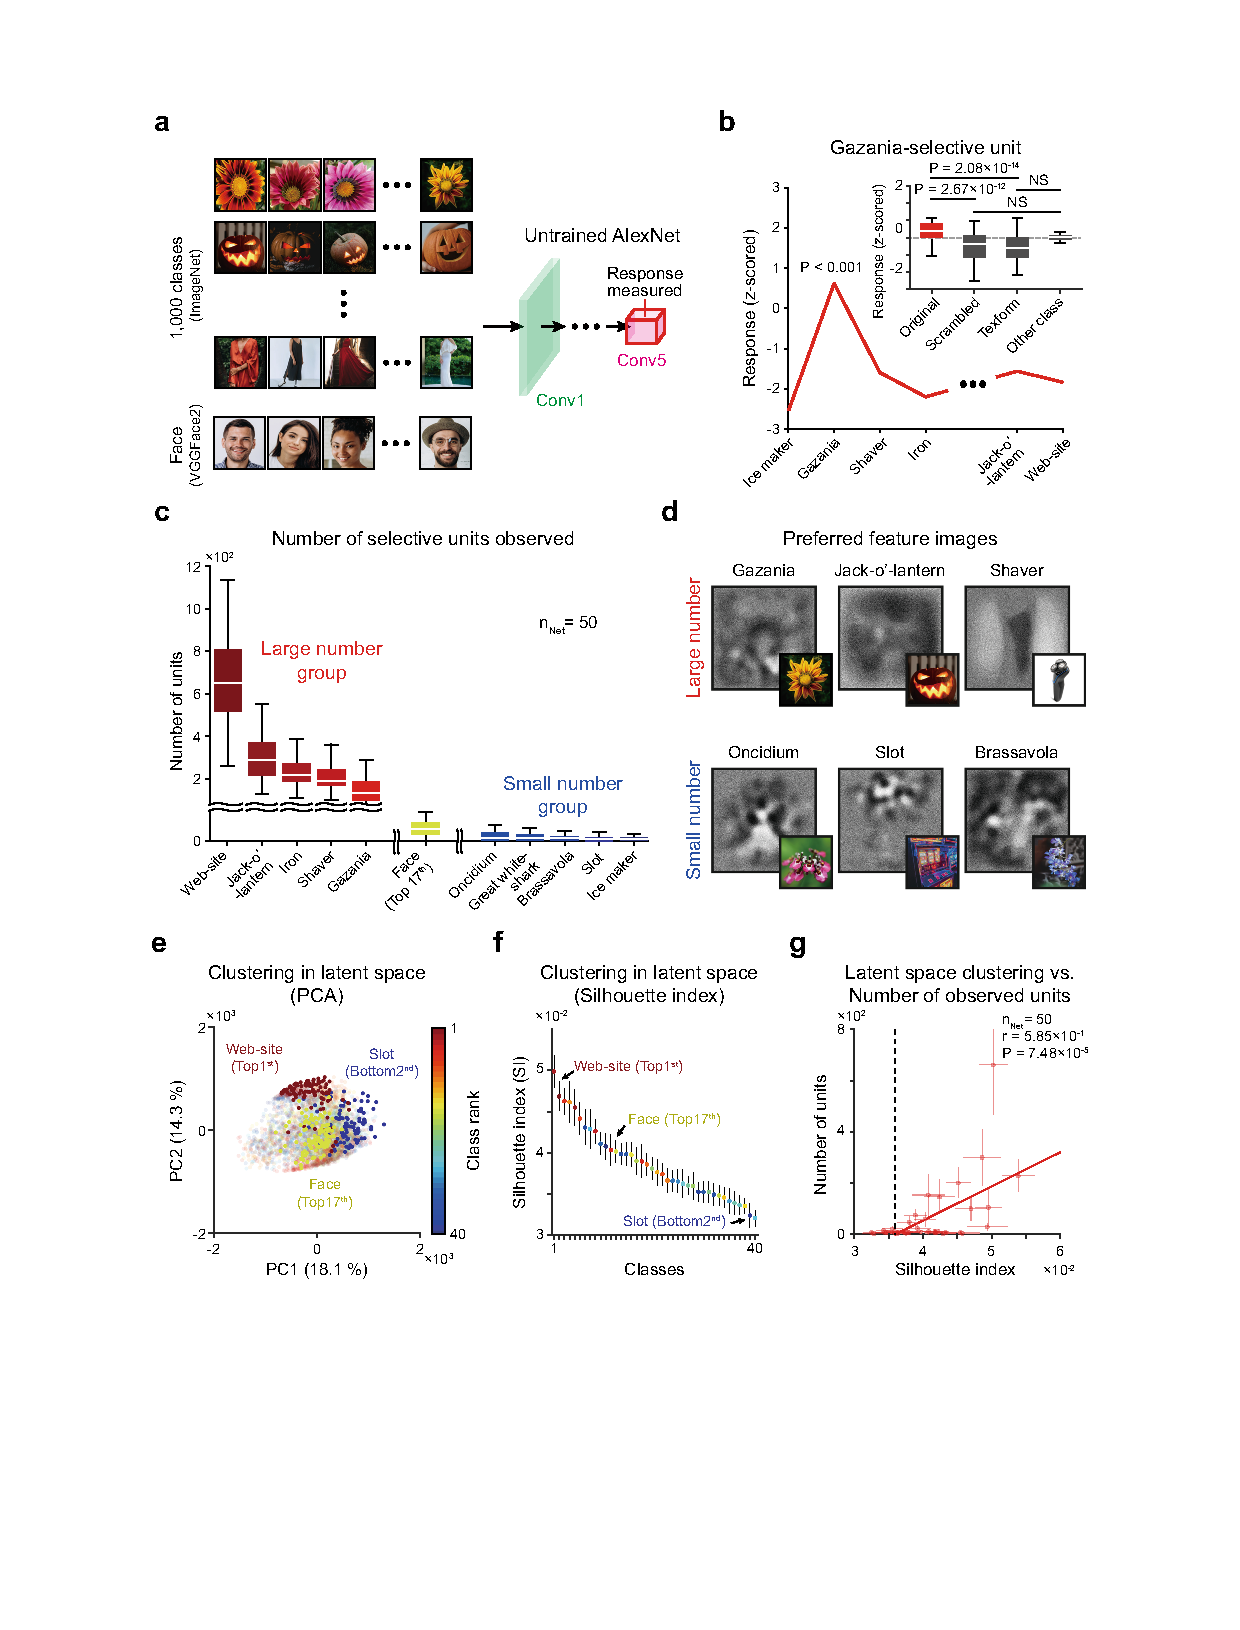
\includegraphics[width=1.0\textwidth]{fig/face_5.pdf}
	\caption{
		\textbf{ImageNet category-selective units in untrained networks.
		}
		(\textbf{a}) The responses of units in untrained networks to the images of 1,000 ImageNet~\cite{russakovsky2015imagenet} classes and to face images (VGGFace2)~\cite{cao2018vggface2}.
		% 杂色菊
		(\textbf{b}) Average tuning curve of gazania selective units.
		(Inset) Responses of gazania-selective units to the original gazania ($ n = 100 $), the scrambled gazania ($ n = 100 $) and texform gazania images ($ n = 100 $).
		(\textbf{c}) The number of selective units for 39 classes in which selective units are observed.
		The error bar indicates the standard deviation of 50 random networks.
		%	
		(\textbf{d}) Sample preferred feature images achieved by reverse-correlation analysis and stimulus images (inset).
		% 
		(\textbf{e}) Visualization of the PCA (principal component analysis)~\cite{wold1987principal} analysis results (only two principal components (PC) are shown) using the Conv5 unit response to each class in untrained networks.
		The analysis was performed using 3,999 principal components, and the top $140 \pm 32$ components contained $ 75\% $ of the variance.
		% 轮廓系数(Silhouette Coefficient),是聚类效果好坏的一种评价方式。
		(\textbf{f}) The silhouette index~\cite{kaufman2009finding} of the Conv5 unit responses was measured using all principal components to estimate the consistency of data clustering.
		Each dot indicates the mean and the error bar indicates the standard deviation of 50 simulations of randomly initialized networks.
		% 
		(\textbf{g}) Correlation between the silhouette index and the number of selective units observed (Pearson correlation).
		Each dot indicates the mean and the error bar indicates the standard deviation of 50 random networks.
		%
		All box plots indicate the inter-quartile range (IQR between Q1 and Q3) of the dataset, the horizontal line depicts the median and the whiskers correspond to the rest of the distribution (Q1-1.5*IQR, Q3+1.5*IQR).
		For copyright reasons, the images in panels (\textbf{a}) and (\textbf{d}) are not the actual images used in the experiments.
		The original images are replaced with images with similar contents for display purposes.
		The original images are available at [\url{https://www.image-net.org/download}, \url{https://arxiv.org/abs/1710.08092}].
		Images shown are available at [\url{https:/www.shutterstock.com}].
	} \label{fig:image_net}
\end{figure}

% 面部
Lastly, we investigated the possibility that units selective to various objects other than faces also emerge similarly in untrained neural networks.
For this, we measured the responses of units in random networks to a stimulus dataset of ImageNet containing 1,000 classes of objects (\ref{fig:image_net}a).
As a result, we found that selective units are observed in 39 classes among the 1,000 classes (\ref{fig:image_net}b,c).
From the analysis using scrambled and texform control images, we confirmed that these object-selective units are not particularly selective to local image parts but are selective to a whole object, similar with units selective to faces
(\ref{fig:image_net}b, inset,
Gazania vs. Scrambled gazania, 
$ n=100 $,
one-sided rank-sum test,
$ P = 2.67 \times 10^{-12} $,
$ r_\textrm{rbc} = 4.89 \times 10^{-1} $,
%
Gazania vs. Texform gazania, 
$ n = 100 $,
one-sided rank-sum test, NS,
$ P = 1.00 $,
$ r_\textrm{rbc} = 3.17 \times 10^{-1} $,
one-sided Kolmogorov-Smirnov test,
$ P = 1.02 \times 10^{-2} $,
$ d = 2.97 \times 10^{-2} $;
% 
Texform gazania vs. other-class,
$ n = 100 $,
one-sided Kolmogorov-Smirnov test,
$ P = 3.45 \times 10^{-2} $,
$ d = 2.55 \times 10^{-2} $
).
This result suggests that units selective innately to various objects such as faces can emerge in untrained neural networks.


Next, to investigate the emergent condition of units selective to each object further, we sorted those 39 classes according to the number of selective units observed and computed the PFI using the RC method (\ref{fig:image_net}c,d).
In general, we observed a tendency in which the PFIs of the large number group showed a relatively simple configuration of each preferred object class that was visually observable (\ref{fig:image_net}d, top), 
whereas those of the small number classes represented a more complicated structure of the PFI (\ref{fig:image_net}d, bottom).
From this result, we hypothesized that objects with a simple configuration, such as faces, can induce stronger clustering in the latent space representation than those of other object classes and therefore may have a greater likelihood of generating units selective to them.
To validate our hypothesis, we used the dimension-reduction method~\cite{wold1987principal} to compare a clustered representation of each object class in terms of the raw pixel values and in the responses of Conv5.
For quantification of the representational clustering of each class, we measured the silhouette index~\cite{kaufman2009finding} to estimate the consistency of data clustering.
We found that there is a strong correlation between the silhouette index in the Conv5 latent space and the number of selective units observed
(\ref{fig:image_net}e-g, Pearson correlation coefficient,
$ n_\textrm{Net} = 50 $,
$ r = 5.85 \times 10^{-1} $,
$ P = 7.48 \times 10^{-5} $
).
This result demonstrates that objects with a simple profile, readily distinguishable from those of other objects statistically, lead to a strong clustering of abstracted responses in the DNN and are more likely to generate units selective to it.
Furthermore, the relationship between the silhouette index and the number of units observed shows that the number of units increases as the silhouette index increases,
with no selective units observed when the silhouette index is below 0.036 (\ref{fig:image_net}g, black dashed line).
This result implies that there may be a threshold of the clustering level in the response embedding space, by which a unit selective to that object class can be defined and observed.
In neuroscience, this may provide a possible explanation of why face-selective neurons are observed in various experiments while neurons selective to other objects are not observed as readily.
Thus, the observed face-selectivity may not be a special case of tuning, 
whereas selectivity to other visual objects can also arise in random networks simply due to the relatively simple configuration of the corresponding geometric components.


% 在未训练的DNN中出现面部选择单元和音乐选择单元
\subsubsection{The emergence of face-selectivity and music-selective units in trained DNNs}


\begin{figure}[!htb]
	\centering
	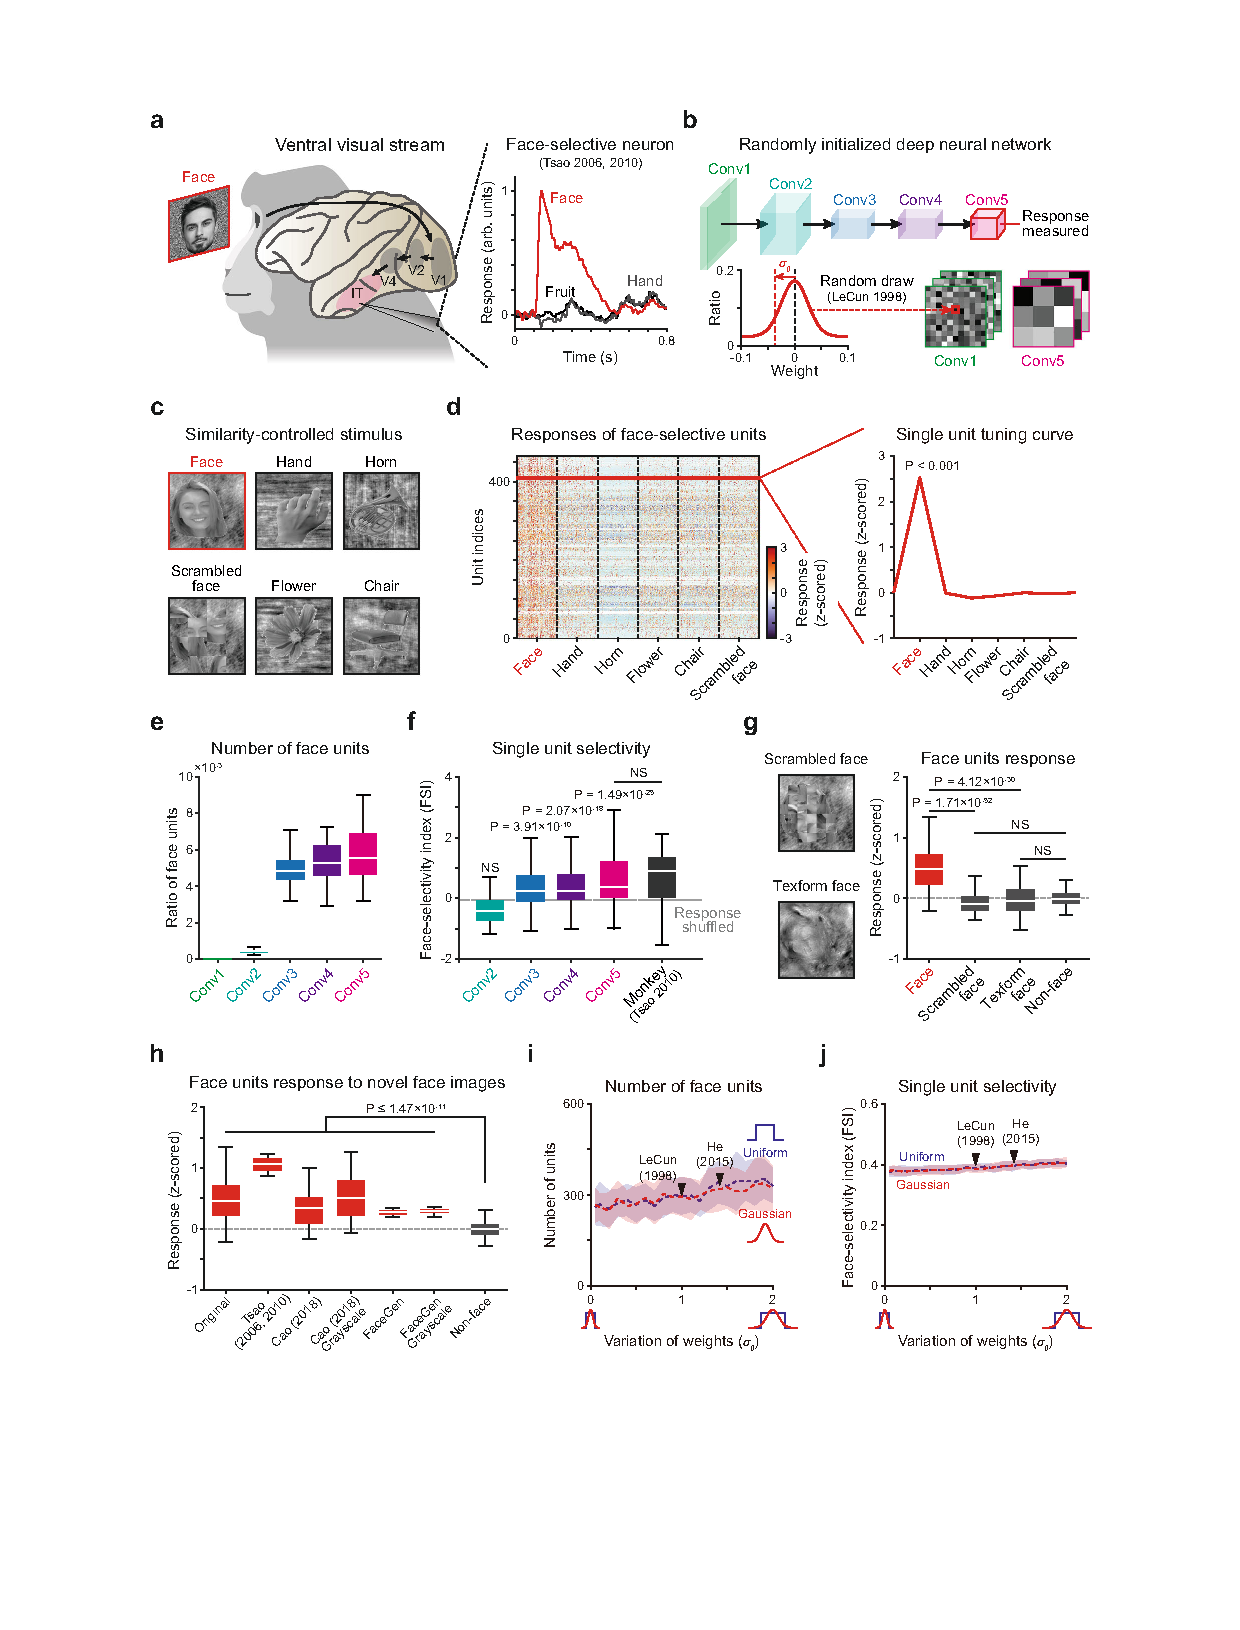
\includegraphics[width=0.9\textwidth]{fig/face_1.pdf}
	\caption{
		\textbf{Spontaneous emergence of face-selectivity in untrained networks.
		}
		\textbf{(a)} Face-select neurons and their response observed in monkey experiments.
		The response was normalized to the maximum value as 1.
		The face image shown is not the original stimulus set due to copyright.
		The image shown is available at \url{https://www.shutterstock.com} (see Methods for details).
		\textbf{(b)} the architecture of the untrained AlexNet~\cite{krizhevsky2012imagenet}.
		The untrained AlexNet was devised using a random initialization method~\cite{lecun2002efficient}, for which the values in each weight kernel were randomly sampled from a Gaussian distribution.
		\textbf{(c)} A stimulus set was designed to control the degree of intra-class image similarity.
		Stimulus images were selected and modified from a publicly available dataset that has been used in human fMRI study~\cite{stigliani2015temporal}.
		The original images are available at [\url{http://vpnl.stanford.edu/fLoc/}].
		\textbf{(d)} Responses of individual face-selective units in the untrained AlexNet ($ P < 0.001 $, two-sided rank-sum test, uncorrected).
		\textbf{(e)} The number of face-selective units in each convolutional layer in untrained networks ($ n=100 $).
		% 面部选择单元的面部选择指数
		\textbf{(f)} Face-selectivity index (FSI) of face-selective neurons in the primate IT~\cite{freiwald2010functional} ($ n=158 $), and face units in each convolutional layer in the untrained AlexNet.
		The control FSI was measured according to the shuffled responses of face-selective units in the untrained network.
		% 和打乱的人脸响应进行对比
		\textbf{(g)} (Left) Examples of texform and scrambled face images.
		(Right) Responses of face-selective units to the original face ($ n = 200 $), the scrambled face ($ n=200 $) and texform face images ($ n = 100 $).
		\textbf{(h)} Responses of face-selective units to four different sets of novel face images: 
		(1) 50 face images from our original dataset (images not used for finding face-selective units),
		(2) 16 images used in Tsao et al.~\cite{tsao2006cortical,freiwald2010functional},
		(3) 50 images used in Cao et al.~\cite{cao2018vggface2} in color and gray scale,
		and (4) 50 face images artificially generated by the FaceGen simulator (singular inversions) in color and gray scale. % Singular Inversions (软件公司)
		\textbf{(i)} The number of face-selective units, where the weight variation was changed from 5 to 200\% of the original value using two different initialization methods with Gaussian (red) and a uniform distribution (blue).
		\textbf{(j)} FSI of face-selective units across changes in the weight.
		Dashed lines indicate the mean and shaded areas indicate the standard deviation of 30 random networks.
		% 针对所有图进行说明
		All box plots indicate the inter-quartile range (IQR between Q1 and Q3) of the dataset,
		% 第三四分位数与第一四分位数的差距又称四分位距(InterQuartile Range, IQR)
		the horizontal line depicts the median and the whiskers correspond to the rest of the distribution (Q1-1.5*IQR, Q3+1.5*IQR).
	} \label{fig:emergence}
\end{figure}



% 人脸选择单元
To simulate the emergence of face-selective neurons, we measured the responses of a biologically inspired DNN model, AlexNet\cite{krizhevsky2012imagenet}, to a similarity-controlled face simulus set.
A standard AlexNet model is composed of five convolutional layers (feature extraction network) and three fully connected layers (classification network), which together reproduce the structure of the ventral stream of the visual pathway (\ref{sec:nn}).
To investigate the selective response of individual units rather than the performance of a trained system, 
we discard the classification layers and examined activity in the final layer (\ref{fig:emergence}b,top,Conv5) of the feature extraction network.
To examine whether face tuning of units can arise even in completely untrained DNNs, 
we devised an untrained AlexNet by randomly initializing the weights of filters in each convolutional layer (\ref{fig:emergence}b, bottom).
% 控制输入信号的长度?
For this, we used a standardized network initialization method~\cite{lecun2012efficient}, by which the weights of kernels in each convolutional layer were randomly drawn from a Gaussian distribution with parameters set to control the strength of the input signals across layers.
The stimulus set consisted of grayscale images in six different categories (\ref{fig:emergence}c), specifically the face, a scrambled face, and four non-face objects, as previously done in monkey experiments~\cite{stigliani2015temporal}.
The images in each class were designed to control the low-level features of the luminance, contrast, object size, and object location, and they have statistically comparable intra- and inter-class image levels of similarity.


% 观察到的现象
Surprisingly, we observed a group of face-selective units ($ n = 250 \pm 63 $ in 100 random networks, mean $ \pm $ s.d.) that show significantly higher response to face images than to non-face images emerging in the untrained networks (\ref{fig:emergence}d, $ P<0.001 $, two-sided rank-sum test).
Here, a unit is defined as a unit component at each position of the channel in an activation map of the network.
For example, there are 43,264 units (=13$\times$13$\times$256, $ N_{x-position} \times N_{y-position} \times N_{channel} $) in Conv5.
We considered each unit (of the same filter) at different spatial locations as different ones, as the selectivity of units at different locations appears to be distinct despite the fact that they share the same filter.
We also investigated the layer-specific emergence of face-selective units in untrained networks.
We found that face-selective units are also observed in earlier layers, Conv3 to 5 but are scarcely found in Conv1 and 2 (\ref{fig:emergence}e, 
Conv1: $ n=0.008 \pm0.002\% $, 
Conv2: $ n=0.047 \pm 0.009\% $, 
Conv3: $ n=0.491 \pm 0.089\% $, 
Conv4: $ n=0.534 \pm 0.103\% $,
Conv5: $ n=0.579 \pm 0.146\% $).
We found that the number of face-selective units and the face-selectivity index (FSI) of each unit increased through the layer hierarchy (\ref{fig:emergence}e,f).
Notably, the number of face-selective units did not show significant differences across the convolutional group or filters within each layer.
This suggests that face-selective units are not dominantly generated by a particular filter.
The number of observed face-selective units was highest in the mid- and high-level layers, similar to observations in the ventral visual pathway of monkeys~\cite{tsao2006cortical,livingstone2017development}.
These results suggest that the development of face-selectivity requires a hierarchical structure of the network along with random feedforward weights, which enables multiple linear-nonlinear computations.
We also found that the observed face-selective units in the untrained networks (Conv5) show a value of the averaged FSI~\cite{tsao2006cortical,freiwald2010functional} comparable to the index associated with monkey IT neurons (\ref{fig:emergence}f, $ n_{untrained} = 465 $, $ n_{monkey} = 158 $, NS, two-sided rank-sum test, $ P=7.69 \times 10 ^{-2} $, $ r_{rbc} = 9.25 \times 10^{-2} $, two-sided Kolmogorov-Smirnov test, $ P=2.49 \times 10^{-4}, d=2.32 \times 10^{-2} $)
and a significantly higher value that those measured from a shuffled response (\ref{fig:emergence}f, $ n_{untrained} = 465 $, $ n_{shuffled} = 465 $, two-sided rank-sum test, $ P=1.49 \times 10^{-25}, r_{rbc} = 5.09 \times 10^{-1} $) for various definitions of the FSI~\cite{tsao2006cortical,aparicio2016neurophysiological,duyck2021color}.
These results suggest that face-selective units, highly tuned to the face as observed in the brain, can emerge in DNNs even in the complete absence of learning.


One possible scenario for the emergence of such face-selectivity in random networks is that the observed face-selective units are simply sensitive for local face parts common to facial images.
To investigate this possibility, we measured the responses of the face-selective units to a local feature of the face using two types of control images in which global face features are disrupted but local face features are preserved.
These were (1) scrambled faces, in which small patches of the local face components were spatially scrambled, and (2) texform face~\cite{long2018mid}, in which global face features are disrupted but the statistics of the local face texture is preserved (\ref{fig:emergence}g,left).
We confirmed that face-selective units show significantly higher responses to the original face images compared to the corresponding control images (\ref{fig:emergence}g, right; 
Face vs. Scrambled face, $ n=200 $, one-side rank-sum test, $ P=1.71 \times 10^{-52} $, $ r_{rbc}=7.69 \times 10^{-1} $;
Face vs. Texform face, $ n=100 $, one-sided rank-sum test, $ P=4.12\times10^{-30} $, $ r_{rbc}=6.56\times 10^{-1} $).
In addition, the responses of face units to these control images were not greater than those to other non-face images, implying that face-selective units are selective to the global context of faces instead of the local components (\ref{fig:emergence}g, right; Scrambled face vs. Non-face, $ n=200 $, one-sided Kolmogorov-Smirnov test, $ P=8.31 \times 10^{-1} $, $ d=3.00 \times 10^{-3} $; 
Texform face vs. Non-face, $ n=100 $, one-sided rank-sum test, NS, $ P=9.40 \times 10^{-1} $, $ r_{rbc}=4.51 \times 10^{-2} $, $ d=1.84 \times 10^{-2} $).
These results suggest that the observed face units in the untrained network are not particularly selective to local face parts, but are instead selective to a whole face.


% h
Next, we investigated the responses of face-selective units to four different novel stimulus sets that were not used to find face-selective units.
These were
(1) 50 face images from our original data set, not used for finding the face-selective units;
(2) 15 face image used in Tsao et al.~\cite{tsao2006cortical,freiwald2010functional};
(3) 50 face images used in Cao et al.~\cite{cao2018vggface2};
and (4) 50 face images artificially generated by the FaceGen simulator (singular inversions) in color and grayscale (\ref{fig:emergence}h).
We found that face-selective units in the untrained network show significantly higher responses to novel face images compared to the responses to non-face under all conditions (\ref{fig:emergence}h, Novel face vs. Non-face images, one-sided rank-sum test, $ P \leq 1.47 \times 10^{-11} $, $ r_{rbc} \geq 4.54 \times 10^{-1}$).
These results suggests that the observed face-selectivity in an untrained network defined by one specific dataset can be generalized to other novel sets of faces.


% figure i, j
To confirm that the emergence of face-selective units is not due to the specific initial parameter set but is rather generally observed in an untrained network,
we varied the width of the weight distribution for random network initialization (Gaussian and uniform) from 5 to 200\% of the original standard deviation of the standardized random initialization and examined if face-selective units consistently emerge (\ref{fig:emergence}i,j).
We found that face-selective units consistently arise in the untrained networks across the variation of the parameter.
The number (\ref{fig:emergence}i) and selectivity index (\ref{fig:emergence}j) of observed face units were largely unchanged across a wide range of weight variations and across the wide variation in the width of the weight distribution.
This implies that the emergence of face-selective units in untrained networks is highly robust to variations of the wiring strength.

% 激活
% 在未训练的网络中有 类别 选择性偏好特征
\subsection{Preferred feature of category-selective units in an untrained network} \label{sec:preferred}

\begin{figure}[!htb]
	\centering
	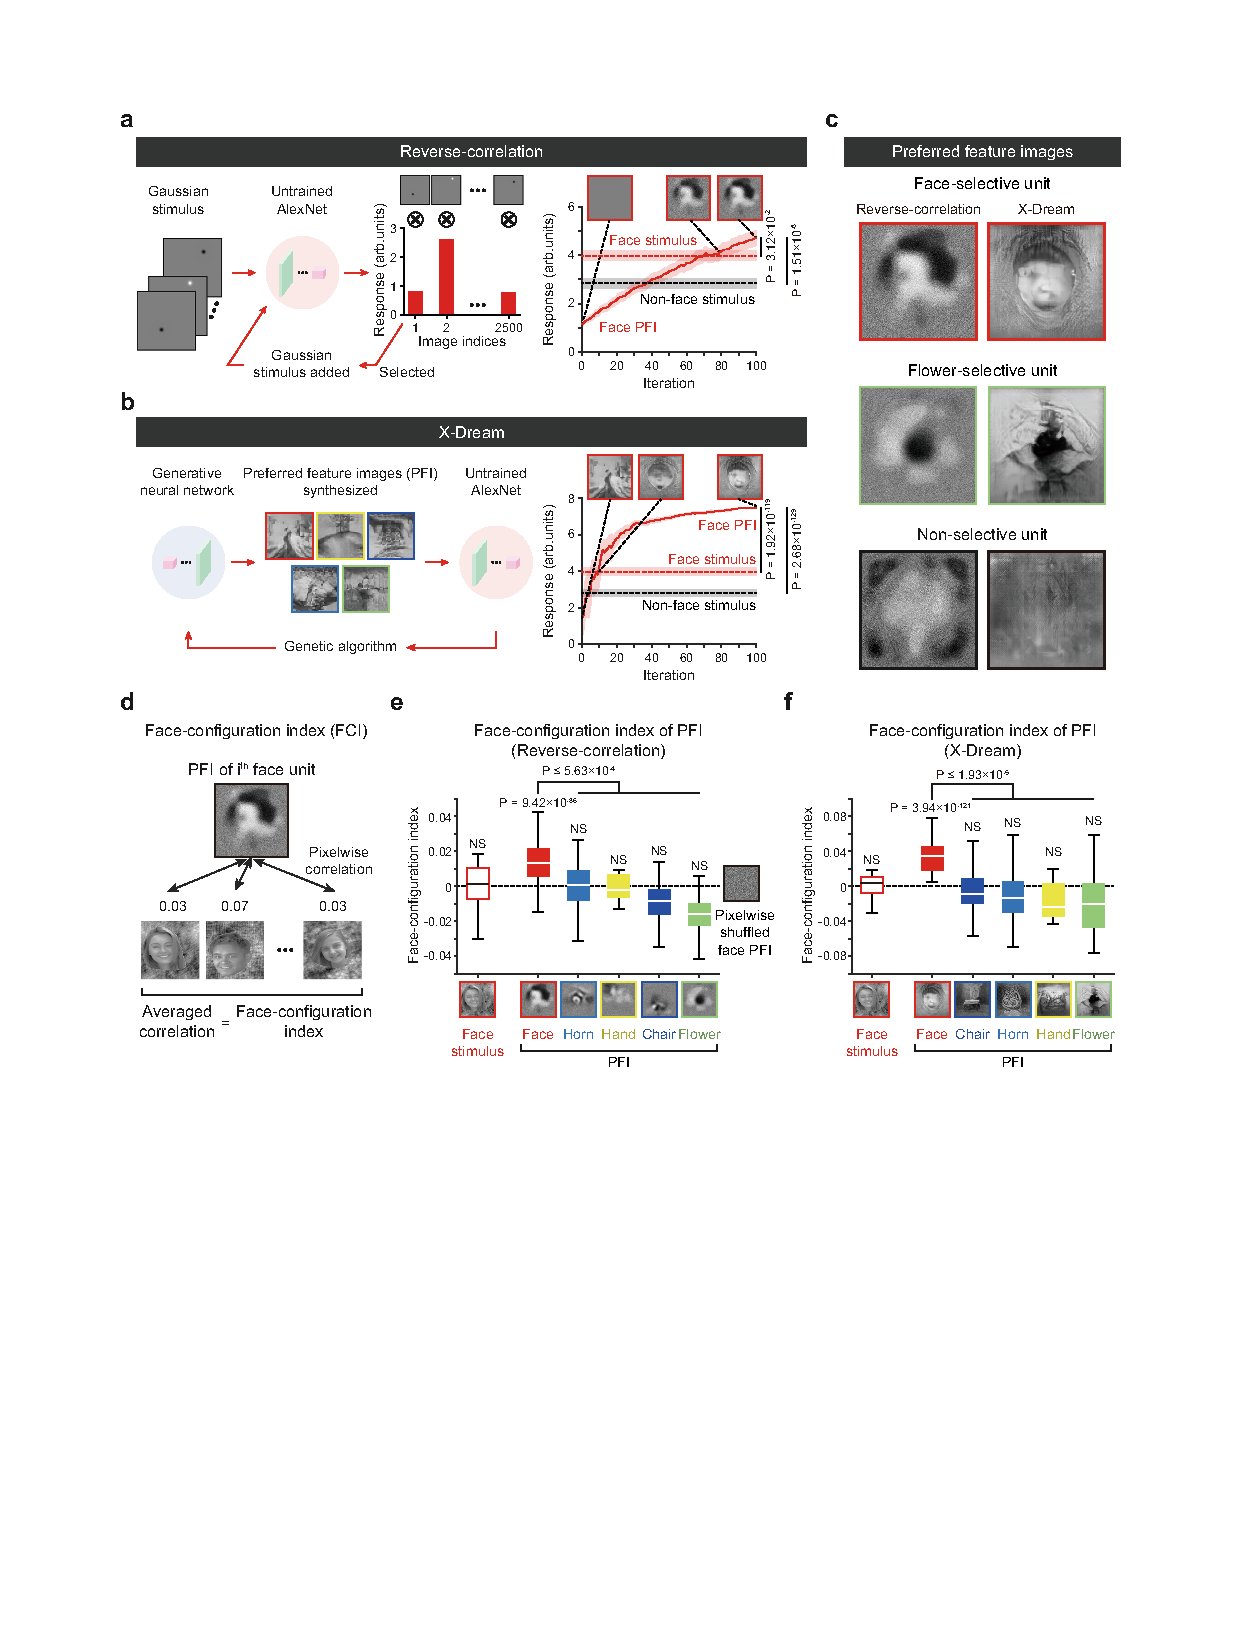
\includegraphics[width=0.9\textwidth]{fig/face_2.pdf}
	\caption{
		\textbf{Preferred feature images of face-selective units in untrained networks.
		}
		\textbf{(a)} Measurements of preferred feature images (PFI) of target units in Conv5 from the reverse-correlation analysis~\cite{bonin2011local}.
		Bright and dark 2D Gaussian filters were generated at a random position as an input stimulus set.
		The PFI was obtained as the summation of stimuli weighted by the corresponding response.
		The initial preferred feature image was calculated from the local Gaussian stimulus set by the classical reverse-correlation method~\cite{bonin2011local}.
		% RNN?
		Then, a new stimulus set was generated as the summation of the obtained PFI and local Gaussian stimuli, with the second preferred feature image then obtained from a new stimulus set.
		This procedure was repeated to obtain the preferred feature image.
		\textbf{(b)} Schematics of the process used to achieve a preferred feature image (PFI) using a generative neural network (GAN) and a genetic algorithm (X-Dream)~\cite{ponce2019evolving}.
		Synthesized images are generated by the GAN with image codes and are fed into an untrained network as input.
		The genetic algorithm finds a new image code that maximizes the response of the target unit.
		The PFI of a target unit is achieved after 100 iterations of this procedure.
		\textbf{(c)} The obtained preferred feature images, using the reverse-correlation method and X-Dream, of the face-selective unit, selective units to non-face class (flower), and units selective to none of the class.
		\textbf{(d)} Illustration of the face-configuration index (FCI) of a face unit's PFI.
		The FCI was defined as pixel-wise correlation between the original face stimuli and the generated PFIs.
		\textbf{(e)} FCI of PFI, using the reverse correlation method, of units selective to each class ($ n_\textrm{Face} = 465 $, $ n_\textrm{Hand} = 7 $, $ n_\textrm{Horn} = 772 $, $ n_\textrm{Flower} = 107 $, $ n_\textrm{Chair} = 63 $).
		\textbf{(f)} FCI of PFI, using X-Dream, of the same units as the units used in (\textbf{e}).
		All box plots indicate the inter-quartile range (IQR between Q1 and Q3) of the dataset,
		the horizontal line depicts the median and the whiskers correspond to the rest of the distribution (Q1-1.5*IQR, Q3+1.5*IQR).
		The face images shown in panels (\textbf{d})-(\textbf{f}) are selected examples from the publicly available dataset~\cite{stigliani2015temporal}.
		The original images are available at [\url{http://vpnl.stanford.edu/fLoc}].
	} \label{fig:preferred}
\end{figure}


Next, to characterize the feature-selective responses of these face-selective units qualitatively,
we reconstructed preferred feature images (PFI) of individual units using a reverse-correlation (RC) method~\cite{bonin2011local} and a generative adversarial network algorithm (X-Dream)~\cite{ponce2019evolving} (see~\ref{sec:preferred}).
In the RC analysis, we presented 2500 images of bright and dard 2D Gaussian filters at random positions as input stimuli to an untrained network (\ref{fig:preferred}).
By adding stimuli weighted according to the corresponding neural response with 100 repeated iterations, we obtained the preferred feature images of the target units.
In the X-Dream analysis, a deep generative adversarial neural network~\cite{dosovitskiy2016generating} was trained to ImageNet datasets to synthesize preferred feature images from the image codes scored by a genetic algorithm using the responses of units from repeated iterations. (\ref{fig:preferred}b).
We found that the response of target units induced by the PFI was increased, being higher that those induced by face stimulus images, as the iteration number of the genetic algorithm exceeds a certain value 
(\ref{fig:preferred}a, right, $ n=465 $, 
RC PFI vs. face stimulus, two-sided rank-sum test, $ P=1.51 \times 10^{-6} $, $ r_{rbc} = 1.58 \times 10^{-1} $;
RC PFI vs. non-face stimulus, two-sided rank-sum test, $ P=3.12 \times 10^{-2} $, $ r_{rbc} = 7.07 \times 10^{-2} $,
\ref{fig:preferred}b, right, $ n=465 $, 
X-Dream PFI vs. face stimulus, two-sided rank-sum test, $ P=1.92 \times 10^{-119} $, $ r_{rbc} = 7.63 \times 10^{-1} $;
X-Dream PFI vs. non-face stimulus, two-sided rank-sum test, $ P = 2.68 \times 10^{-129} $, $ r_{rbc} = 7.94 \times 10^{-1} $
).
These results indicate that our PFI generation methods successfully find the most preferred input feature of face-selective units.
As a result, using both methods, we obtained the PFI of face-selective units, units selective to non-face classes, and units without selective responses to any image classes (\ref{fig:preferred}c).
We found that the PFI of the face-selective units presents distinguishable features from those of other objects.
We observed that the PFIs of face-selective units represent face-like configurations, whereas the PFIs of units selective to non-face classes show noticeable configurations of each object class (i.e., flowers in an RC and X-Dream).


% d
To quantify the structural similarity of the PFIs to face images, we defined the face-configuration index as the averaged pixel-wise correlation between a PFI and the 200 face images used for face unit selection (\ref{fig:preferred}d).
We estimated the face-configuration index of each PFI of face-selective and non-face-selective units generated by the RC method.
We found that the estimated PFIs of face-selective units (with a visually observable face-like configuration) have a significantly higher average value of the index than that from the units selective to non-face objects (\ref{fig:preferred}e, 
Face PFI vs. Non-face PFI, 
$ n_\textrm{Face}    = 465 $,
$ n_\textrm{Horn}    = 772 $,
$ n_\textrm{Hand}    = 7   $,
$ n_\textrm{Chair}   = 63  $,
$ n_\textrm{Flower}  = 107 $,
one-sided rank-sum test,
$ P \leq 5.63 \times 10^{-4} $,
$ r_{rbc} \geq 1.56 \times 10^{-1} $;
\ref{fig:preferred}f, Face PFI vs. Non-face PFI,
$ n_\textrm{Face}   = 465 $,
$ n_\textrm{Chair}  = 63  $,
$ n_\textrm{Horn}	= 773 $,
$ n_\textrm{Hand}	= 7	  $,
$ n_\textrm{Flower}	= 107 $,
one-sided rank-sum test, 
$ P \leq 1.93 \times 10^{-5} $,
$ r_{rbc} \geq 2.35 \times 10^{-1} $
).
Notably, the average pairwise correlation estimated between each face stimulus image shows a significantly lower value of nearly zero, 
implying that the observed index of face-selective units reflects structural similarity to the averaged (or a prototype, abstract) face image rather than similarly to particular face images accidentally observable.


Next, we hypothesized that the observed face-selective units may encode invariant representations of the prototype face images, as some types of intrinsic are a basic property of CNNs.
A number of previous studies suggested that various types of invariance (e.g., translation, scaling, and rotation) over a wide range of image transformations can be implemented in a CNN~\cite{lecun2004learning,kavukcuoglu2010learning,lecun2012learning,chidester2018rotation,srivastava2018effect}, mostly due to three key components--the convolutional layer, the pooling layer, and the hierarchical structure--in CNN models.
Thus, to investigate whether the observed face-selective units show invariant representations of face images regardless of corresponding image condition, 
we measured the response of face-selective units to face and non-face object images with various positions, sizes, and rotation angles.
First, we observed that single face units show constant face tuning under a fairly wide range of size/potion/rotation variations and that range was comparable with those of face-selective neurons in IT~\cite{zoccolan2007trade}.
Notably, we found that our model units also show the inversion effect observed in monkeys~\cite{tsao2006cortical,buiatti2019cortical,perrett1985visual}.
We found that the response of face-selective units to inverted face images are significantly lower that those to upright faces.


% 在随机网络中发现视角不变性的面部选择单元
Similarly, we found viewpoint-invariant face-selective units and mirror-symmetric viewpoint-specific units in a random network.
Interestingly, the number of viewpoint-invariant face-selective units increased along the network hierarchy, similar to previous observations in the brain~\cite{freiwald2010functional}.
These results show that the observed invariances can arise from the hierarchical structure with convolutional filtering without the contribution of structured spatial filters.
Notably, the current result also suggests a possible scenario through which to understand how viewpoint invariant selectivity can arise in infant animals.
From the similarities between the CNN and the biological brain models, i.e., that the fundamentals of both CNNs and sensory cortices are based on the hierarchical feedforward structure and that the process of convolution via weight sharing in CNNs can be approximated by a biological model of periodic functional maps with hypercolumns in the visual cortex,
our result may inspire insight into how innate invariance can arise in infant animals.


% 几何模式限制神经网络激活
\subsection{Geometric modes constrain artificial neural network activity}\label{subsec2}

% 全局的波传到人脸识别区出现的模式响应 vs 人脸识别模式
% 人脸识别区域几何模式(外形)来重建 人脸识别区域 的激活
% 使用人脑的几何特征模式预测人工神经网络的激活
\begin{figure}[!htb]
	\centering
	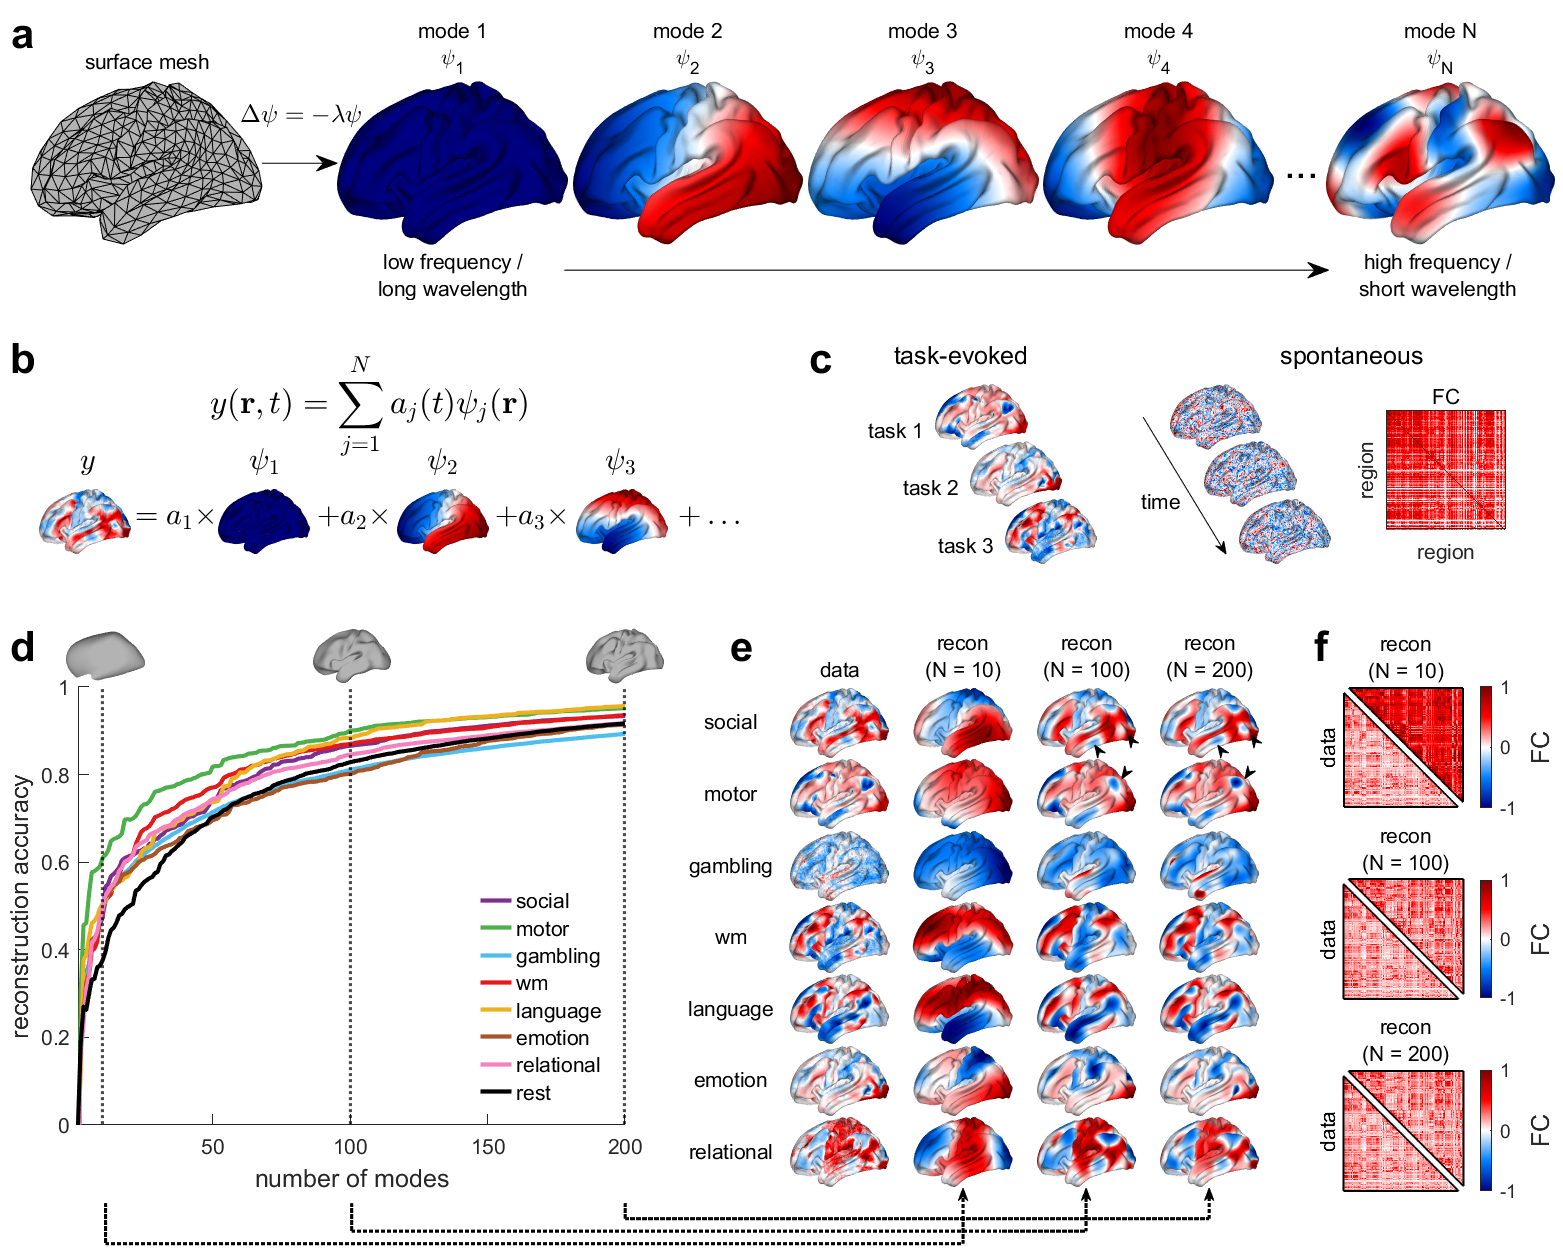
\includegraphics[width=0.9\textwidth]{fig/fig_1.pdf}
	\caption{\textbf{Reconstruction of artificial neural network activity with geometric eigenmodes.}
	\textbf{a}, Geometric eigenmodes are derived from the cortical surface mesh by solving the eigenvalue problem,$ \Delta \psi = -\lambda \psi $ (equation (\ref{eq:1})). 
	The modes $ \psi_1, \psi_2, \psi_3, ... \psi_N $ are ordered from low to high spatial frequency (long to short spatial wavelengths). 
	Negative, zero and positive values are coloured blue, white and red, respectively.
	\textbf{b}, Modal decomposition of brain activity data. 
	The example shows how a spatial map, $ y(r,t) $, at a given time, $ t $, can be decomposed as a sum of modes, $ \psi_j $, weighted by $a_j$.
	\textbf{c}, Left, we reconstruct task-evoked data using spatial maps of activation for a diverse range of stimulus contrasts. 
	Right, we reconstruct spontaneous activity by decomposing the spatial map at each time frame and generating a region-to-region FC matrix.
	\textbf{d}, Reconstruction accuracy of seven key HCP task-contrast maps (Supplementary Information~\ref{sec:sup_2_1}) and restingstate FC as a function of the number of modes. 
	Insets show cortical surface reconstructions, demonstrating the spatial scales relevant to the first 10, 100 and 200 modes corresponding to spatial wavelengths of approximately 120, 40 and 30 mm, respectively.
	\textbf{e}, Group-averaged empirical task-activation maps and reconstructions (recon.) obtained using 10, 100 and 200 modes of the seven key HCP task contrasts. 
	Black arrowheads indicate localized activation patterns that are more accurately reconstructed when using short-wavelength modes. 
	\textbf{f}, Group-averaged empirical resting-state FC matrices and reconstructions using 10, 100 and 200 modes.
	} \label{fig:1}
\end{figure}

We first examine the degree to which geometric eigenmodes can explain diverse aspects of human neocortical activity. 
To derive the eigenmodes, we use a mesh representation of a population-averaged template of the neocortical surface (Fig.~\ref{fig:1}a and Derivation of cortical geometric eigenmodes in Methods). 
We then construct the Laplace– Beltrami operator (LBO) from this surface mesh, which captures local vertex-to-vertex spatial relations and curvature, and solve the eigenvalue problem,
\begin{equation} \label{eq:1}
	\nabla^2 \psi = \Delta\psi = -\lambda \psi,
\end{equation}
where $ \nabla $ is the gradient operator, $ \Delta $ is the LBO and $ \psi = \{\psi_1(r), \psi_2(r),...\} $ is the family of geometric eigenmodes with the corresponding family of eigenvalues $ \lambda = \{ \lambda_1, \lambda_2, ... \} $. 
The eigenvalues are ordered sequentially according to the spatial frequency or wavelength of the spatial patterns of each mode (Fig.~\ref{fig:1}a~and Extended Data Fig.~\ref{fig:extended_fig_1}), such that $ \psi_1 $ is the mode with the longest wavelength. 
The resulting eigenmodes are orthogonal, forming a complete basis set to decompose spatiotemporal dynamics unfolding on the cortex as a weighted sum of modes with varying wavelengths (Fig.~\ref{fig:1}b~and Modal decomposition of brain activity in Methods).
Unless otherwise specified, we use $ N=200 $ modes throughtout this study.


Using this decomposition we evaluate the accuracy of geometric eigenmodes in capturing both task-evoked and spontaneous brain activity (Fig.~\ref{fig:1}c) measured in 255 healthy individuals from the Human Connectome Project27 (HCP; HCP data in Methods and Supplementary Information 2). 
For task-evoked activity, we map 47 task-based contrasts drawn from seven different tasks representing distinct evoked activation patterns. 
We then reconstruct each individual’s activation map using an increasing number of modes up to a maximum of 200 (Fig.~\ref{fig:1}d). 
For spontaneous, task-free (so-called resting-state) activity, we reconstruct the spatial map of activity at each time frame and then generate a region-to-region functional coupling (FC) matrix, describing correlations of activity among 180 discrete brain regions per hemisphere28. 
To allow direct comparison between task-evoked and spontaneous recordings, we apply the same regional parcellation to the task-evoked data (Cortical parcellations in Methods). 
Finally, we quantify reconstruction accuracy by calculating the correlation between empirical and reconstructed task-evoked activation maps and spontaneous FC matrices (Fig.~\ref{fig:1}d-f).


We observe that reconstruction accuracy increases with an increasing number of modes across all task contrasts and in the resting state, with $ r \ge 0.38 $ already achieved using just $ N=10 $ modes (Fig.~\ref{fig:1}d). 
Large-scale modes are also differentially recruited across different tasks, suggesting that particular stimuli excite specific modes (Fig.~\ref{fig:1}e). 
Improvements in reconstruction accuracy become slow after ten modes, reaching $ r \geq 0.80 $ at approximately $ N=100 $ modes, with only incremental increases in reconstruction accuracy beyond this point. 
Beause the first 100 modes have wavelengths above around 40 mm (Supplementary Table~\ref{tab:spatial_wavelength}), 
and the inclusion of shorter-wavelength modes only refines reconstruction of localized patterns (arrowheads in Fig.~\ref{fig:1}e), our findings suggest that the data are predominantly comprised of spatial patterns with long spatial wavelengths (see next section for a more detailed analysis).


These results are consistent across all 47 HCP task contrasts (Supplementary Fig.~\ref{fig:supp_1}) and parcellations of varying resolutions (Supplementary Fig.~\ref{fig:supp_2}), but data parcellated at higher resolution require more modes to achieve high reconstruction accuracy due to the low-pass spatial filtering effect of coarser parcellations. 
Our results are also not affected by the use of a population-averaged cortical surface template (rather than individual-specific surfaces) to derive the geometric eigenmodes (Supplementary Figs.~\ref{fig:supp_3}-\ref{fig:supp_5}~and Supplementary Information~\ref{sec:individual_specific}). 
Together these findings indicate that cortical geometric eigenmodes form a compact representation that captures diverse aspects of task-evoked and spontaneous cortical activity. 
Moreover, they show that such activity is dominated by long-wavelength, large-scale eigenmodes.


We next test the hypothesis that geometric eigenmodes provide a more parsimonious and fundamental description of dynamics than eigenmodes derived from a graph-based connectome approximation. 
To this end we compare the reconstruction accuracy of geometric eigenmodes against three alternative connectome-derived eigenmode basis sets (see Fig.~\ref{fig:2}a~for a schematic). 
The first basis set is derived empirically from a connectome mapped with dMRI tractography at vertex resolution and thresholded to obtain a connection density of  0.10\%, as done previously29 (Derivation of connectome eigenmodes in Methods). 
The second basis set is derived from a connectome constructed synthetically according to a homogeneous stochastic wiring process governed by an exponential distance-dependent connection probability to mimic simple, EDR-like connectivity (Derivation of EDR eigenmodes in Methods). 
Because the connection densities of empirical and EDR connectomes differed, we evaluated a third basis set derived from the empirical connectome thresholded at 1.55\% to match the density of the EDR connectome. 
The connectome, EDR and density-matched connectome eigenmodes described above are derived from the graph Laplacian (a discrete counterpart of the LBO) of their respective connectivity matrices (Fig.~\ref{fig:2}b~and Extended Data Fig.~\ref{fig:extended_fig_1}).


To summarize, geometric eigenmodes account for the intrinsic curvature of the cortical surface and local vertex-to-vertex relations in the surface mesh; 
connectome eigenmodes do not consider curvature but capture local spatial relations between mesh vertices, along with short- and long-range connections measured with dMRI; 
and EDR eigenmodes account for the effect of a homogeneous, stochastic, distance-dependent connection rule without fully capturing the cortical geometry (Fig.~\ref{fig:2}a). 
Contrasting these different basis sets thus allows us to disentangle the contributions to brain dynamics of cortical geometry from structural connectivity.


Direct comparison of the reconstruction accuracy of these different basis sets shows that geometric eigenmodes consistently show the highest reconstruction accuracy across both spontaneous (Fig.~\ref{fig:2}c) and task-evoked (Fig.~\ref{fig:2}d) data. 
EDR eigenmodes perform nearly as well as geometric eigenmodes whereas connectome eigenmodes are the least accurate. 
This finding holds true regardless of the parcellation used (Extended Data Figs.~\ref{fig:extended_fig_2}~and~\ref{fig:extended_fig_3}), the specific connection density used to generate the connectome eigenmodes (Supplementary Figs.~\ref{fig:extended_fig_6}~and~\ref{fig:extended_fig_7}~and Supplementary Information~\ref{sec:thresholding_effect}) and whether we generate the connectome using a discrete regional parcellation rather than at vertex resolution (Supplementary Fig.\ref{fig:extended_fig_8} and Supplementary Information~\ref{sec:thresholding_effect}). 
We additionally find that geometric eigenmodes show stronger out-of-sample generalization than principal components of the functional data themselves (calculated via principal component analysis (PCA); Supplementary Fig.\ref{fig:supp_9}, Extended Data Fig.~\ref{fig:extended_fig_4} and Supplementary Information~\ref{sec:comparison_eigenmodes_derived}) and better performance than Fourier spatial basis sets (Extended Data Fig.\ref{fig:extended_fig_5}, Supplementary Information~\ref{sec:comparison_fourier}~and Comparisons with statistical basis sets in Methods~\ref{sec:sets_comparisons}).

% 长波主导神经网络激活
\subsection{Long wavelengths dominate artificial neural network activity}

\begin{figure}[!htb]
	\centering
	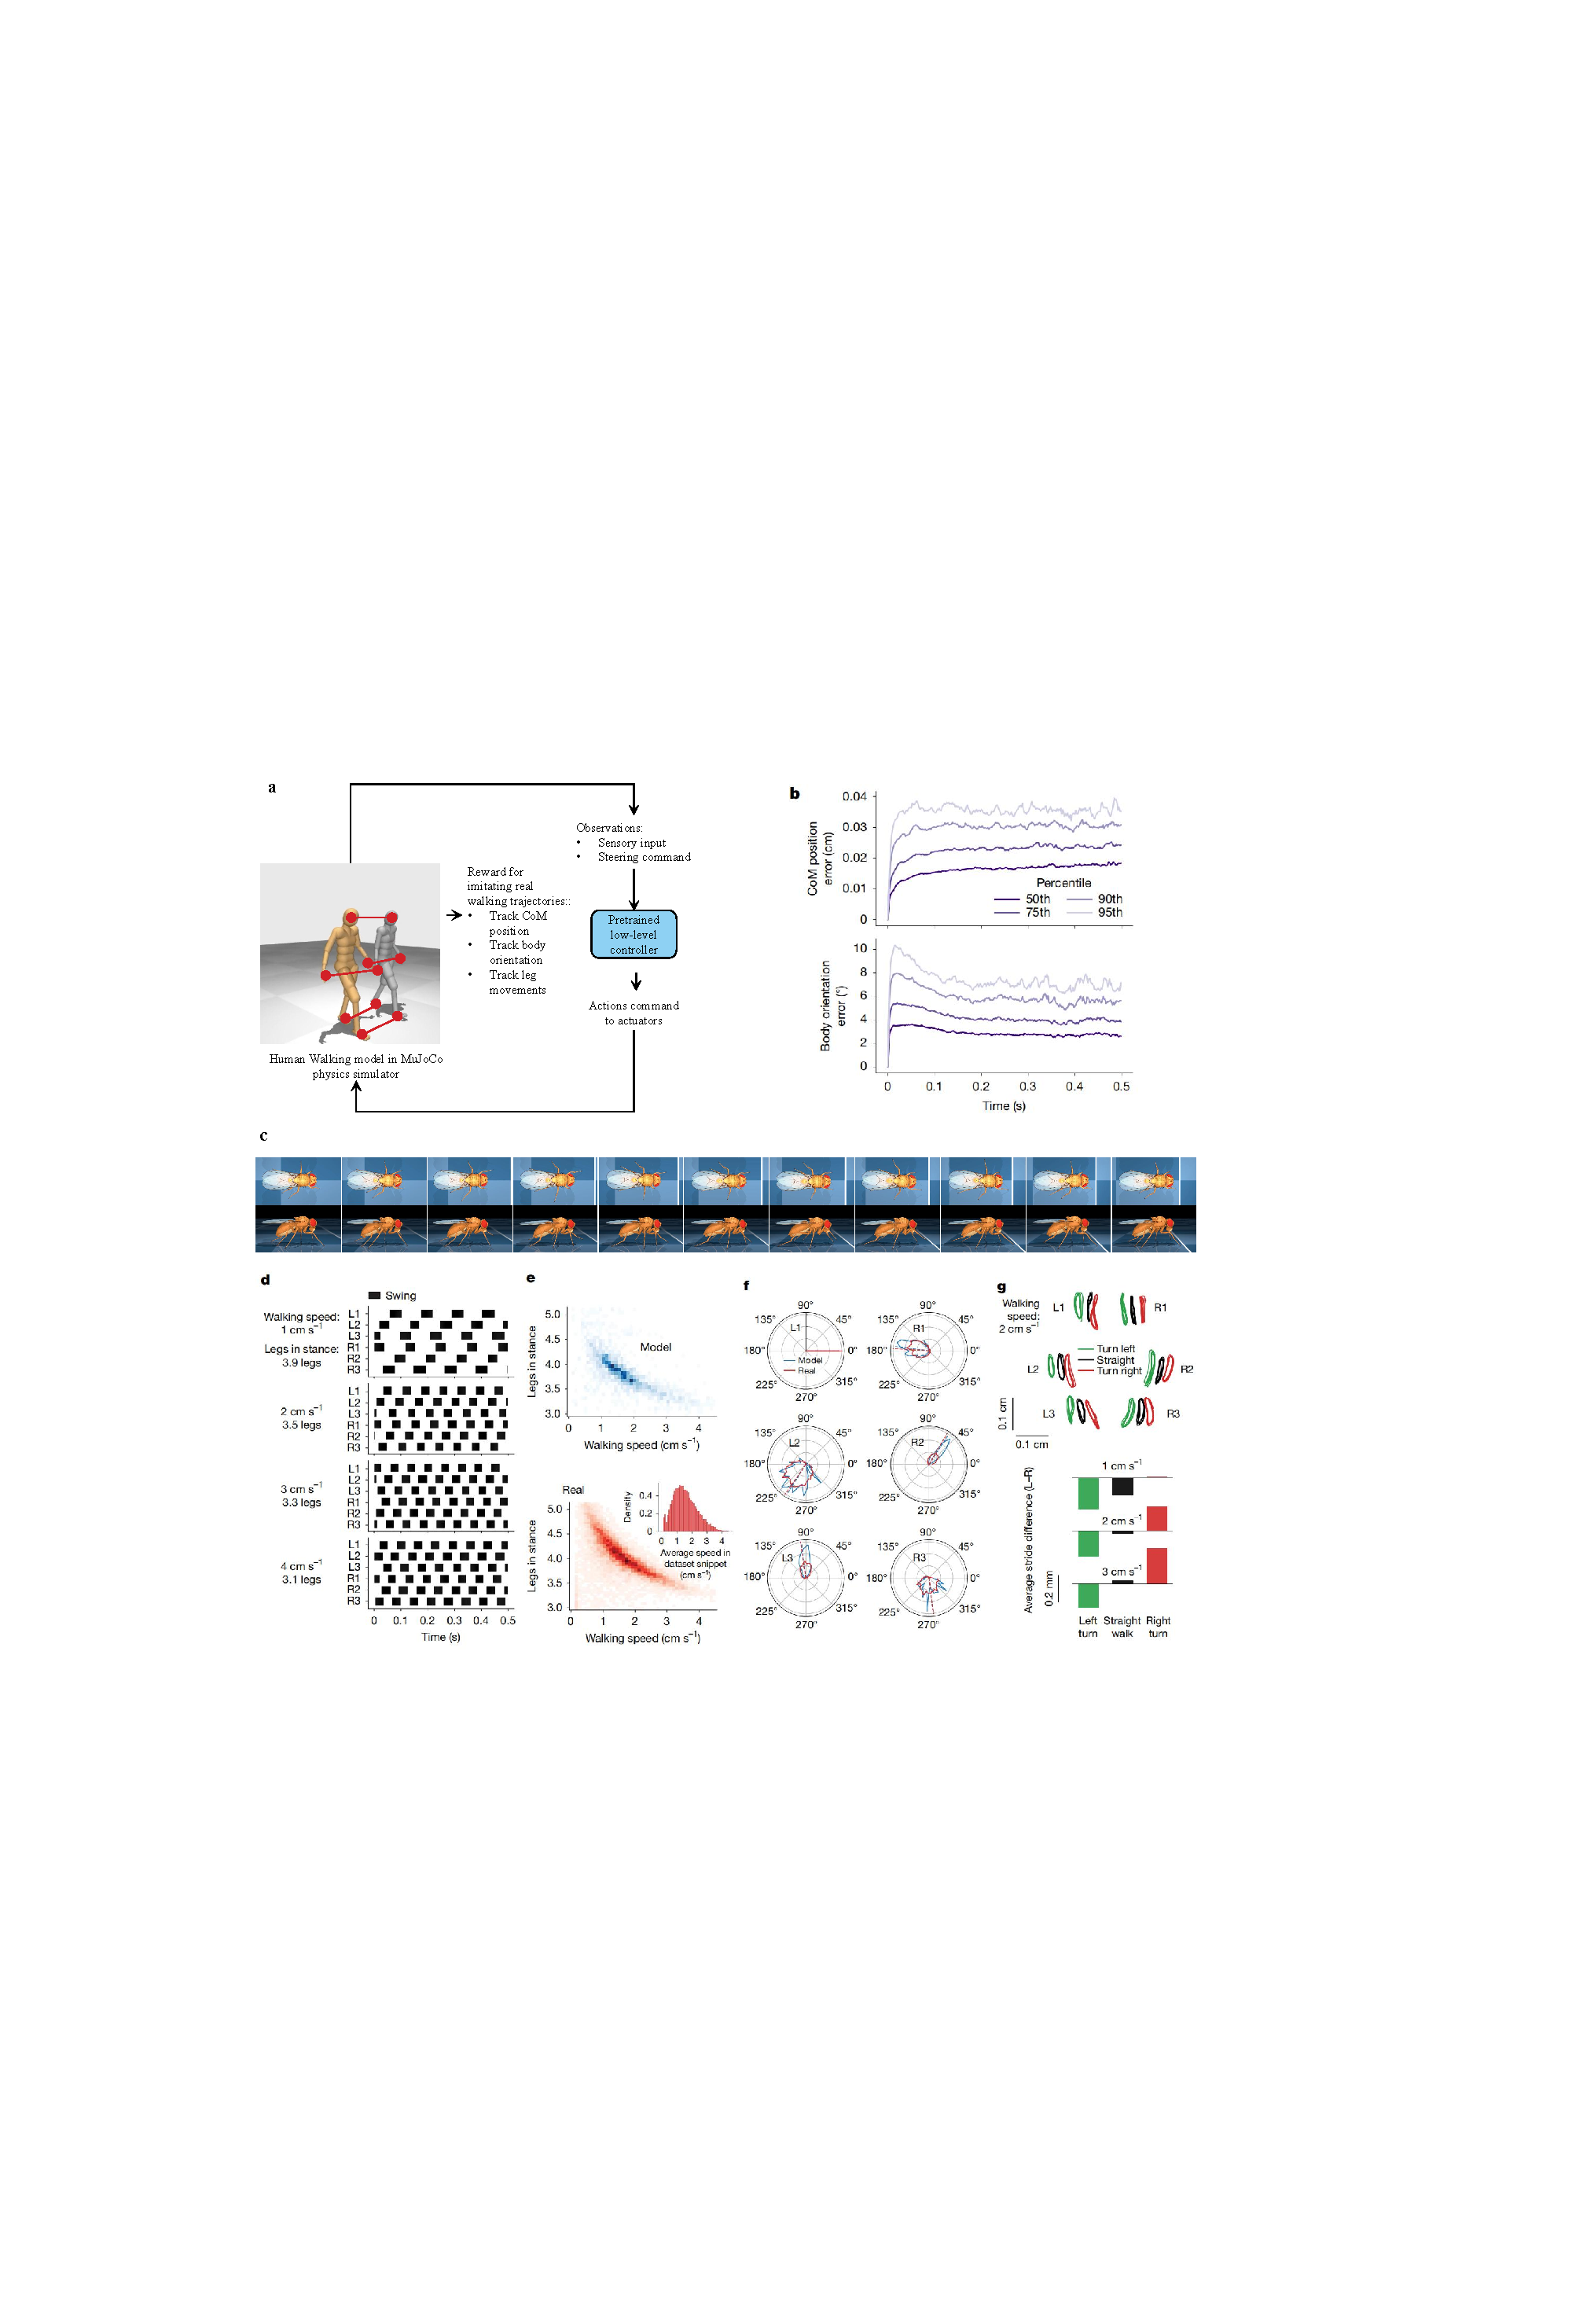
\includegraphics[width=0.9\textwidth]{fig/fig_2.pdf}
	\caption{\textbf{Geometric eigenmodes benchmarked against connectome-based eigenmodes.}
	\textbf{a}, Schematic of the anatomical properties used to derive eigenmodes for cortical geometry, the connectome and the EDR connectome. 
	Geometric eigenmodes rely on local surface mesh information such as links (blue) between neighbouring surface mesh vertices (dots) and curvature. 
	Connectome eigenmodes rely on local links between mesh vertices (blue) and short- and long-range connections (magenta) reconstructed empirically from dMRI. 
	EDR eigenmodes rely on connections (red) generated from a stochastic wiring process in which the probability of connection between vertices exponentially decays as a function of their distance.
	\textbf{b}, Example connectome and EDR eigenmodes. 
	Negative, zero and positive values are coloured blue, white and red, respectively. 
	Despite some similarities, the spatial patterns of the modes are distinct from those derived using cortical geometry (compare with Fig.~\ref{fig:1}a).
	\textbf{c}, Reconstruction accuracy of resting-state FC matrices achieved by geometric, EDR and two variants of connectome eigenmodes: 
	one using a connectome as defined using previous methods\cite{naze2021robustness} and the other with the same connection density as the EDR connectome to allow fair comparison (for other densities see Supplementary Figs.~\ref{fig:supp_6}~and~\ref{fig:supp_7}).
	} \label{fig:2}
\end{figure}


Reconstructions of both spontaneous and task-evoked data with geometric eigenmodes show that the spatial organization of brain activity is dominated by patterns with spatial wavelengths of about 40 mm or longer (Fig.~\ref{fig:1}d–f). 
This result counters classical approaches to analysis of neuroimaging data, in which stimulus-evoked activations are mapped by thresholding statistical maps to identify focal, isolated areas of heightened activity. 
This classical approach rests on the assumption that focal loci represent discrete brain regions putatively engaged by the stimulus and that subthreshold activity in other regions is of negligible interest. 
The surprisingly long-wavelength content of task-activation data (Fig.~\ref{fig:1}d-e) suggests that classical procedures focus only on the tips of the iceberg and obscure the underlying spatially extended and structured patterns of activity evoked by the task (see Extended Data Fig.~\ref{fig:extended_fig_6}~for an explanation of the reasons involved). 
These observations accord with the theoretical predictions of NFT and previous analyses of task-evoked electroencephalography (EEG) signals\cite{robinson2001modal,wingeier2001spherical}.


Here we leverage the modal decomposition described in Fig.~\ref{fig:1}b to characterize the complete spatial pattern—the entire iceberg— of task-evoked activation. 
To this end we analyse the spatial power spectrum obtained using a geometric mode decomposition of group-averaged unthresholded activation maps from the 47 task contrasts in HCP\cite{van2013wu,gorgolewski2015neurovault} (Modal power spectra of task-evoked activation maps in Methods). 
As an independent replication, we also analyse 10,000 unthresholded activation maps from 1,178 independent experiments available in the NeuroVault repository\cite{van2013wu,gorgolewski2015neurovault}, thus providing a comprehensive picture of the diversity of stimulus-evoked activation patterns mapped in the human brain.


Despite the wide range of stimuli, paradigms and data-processing approaches used to acquire these activation maps, we observe that a large fraction of power in the maps is concentrated in the first 50 modes, corresponding to spatial wavelengths greater than around 60 mm (Fig.~\ref{fig:3}a; similar results are found separately for each of the key HCP task-contrast maps; Extended Data Fig.~\ref{fig:extended_fig_7}). 
Using surrogate data, we confirm that these findings cannot be explained by the spatial smoothing  induced by typical fMRI processing pipelines, which can filter out short-wavelength spatial patterns of activity (Extended Data Fig.~\ref{fig:extended_fig_8}~and Supplementary Information~\ref{sec:modal_power_spectra}). 
We further observe that incremental, sequential removal of long-wavelength modes has a much greater impact on reconstruction accuracy than removal of short-wavelength modes (Fig.~\ref{fig:3}b~and Contributions of long- and short-wavelength modes in Methods~\ref{sec:wavelength_contributions}). 
For instance, across the seven key HCP task contrasts, removal of the top 25\% long-wavelength modes (modes 1–50) yields a drop in reconstruction accuracy of around 40–60\% whereas removal of the top 25\% short-wavelength modes (modes 151–200) yields a drop of only around 2–4\% (Fig.~\ref{fig:3}b, insets). 
These results indicate that, on temporal and spatial scales accessible with fMRI, evoked cortical activity comprises large-scale, nearly brain-wide spatial patterns, challenging classical views that such activity should be described in terms of discrete, isolated and anatomically localized activation clusters.


% 波动力学连接和几何和功能
\subsection{Wave dynamics bridge geometry and function}


\begin{figure}[!htb]
	\centering
	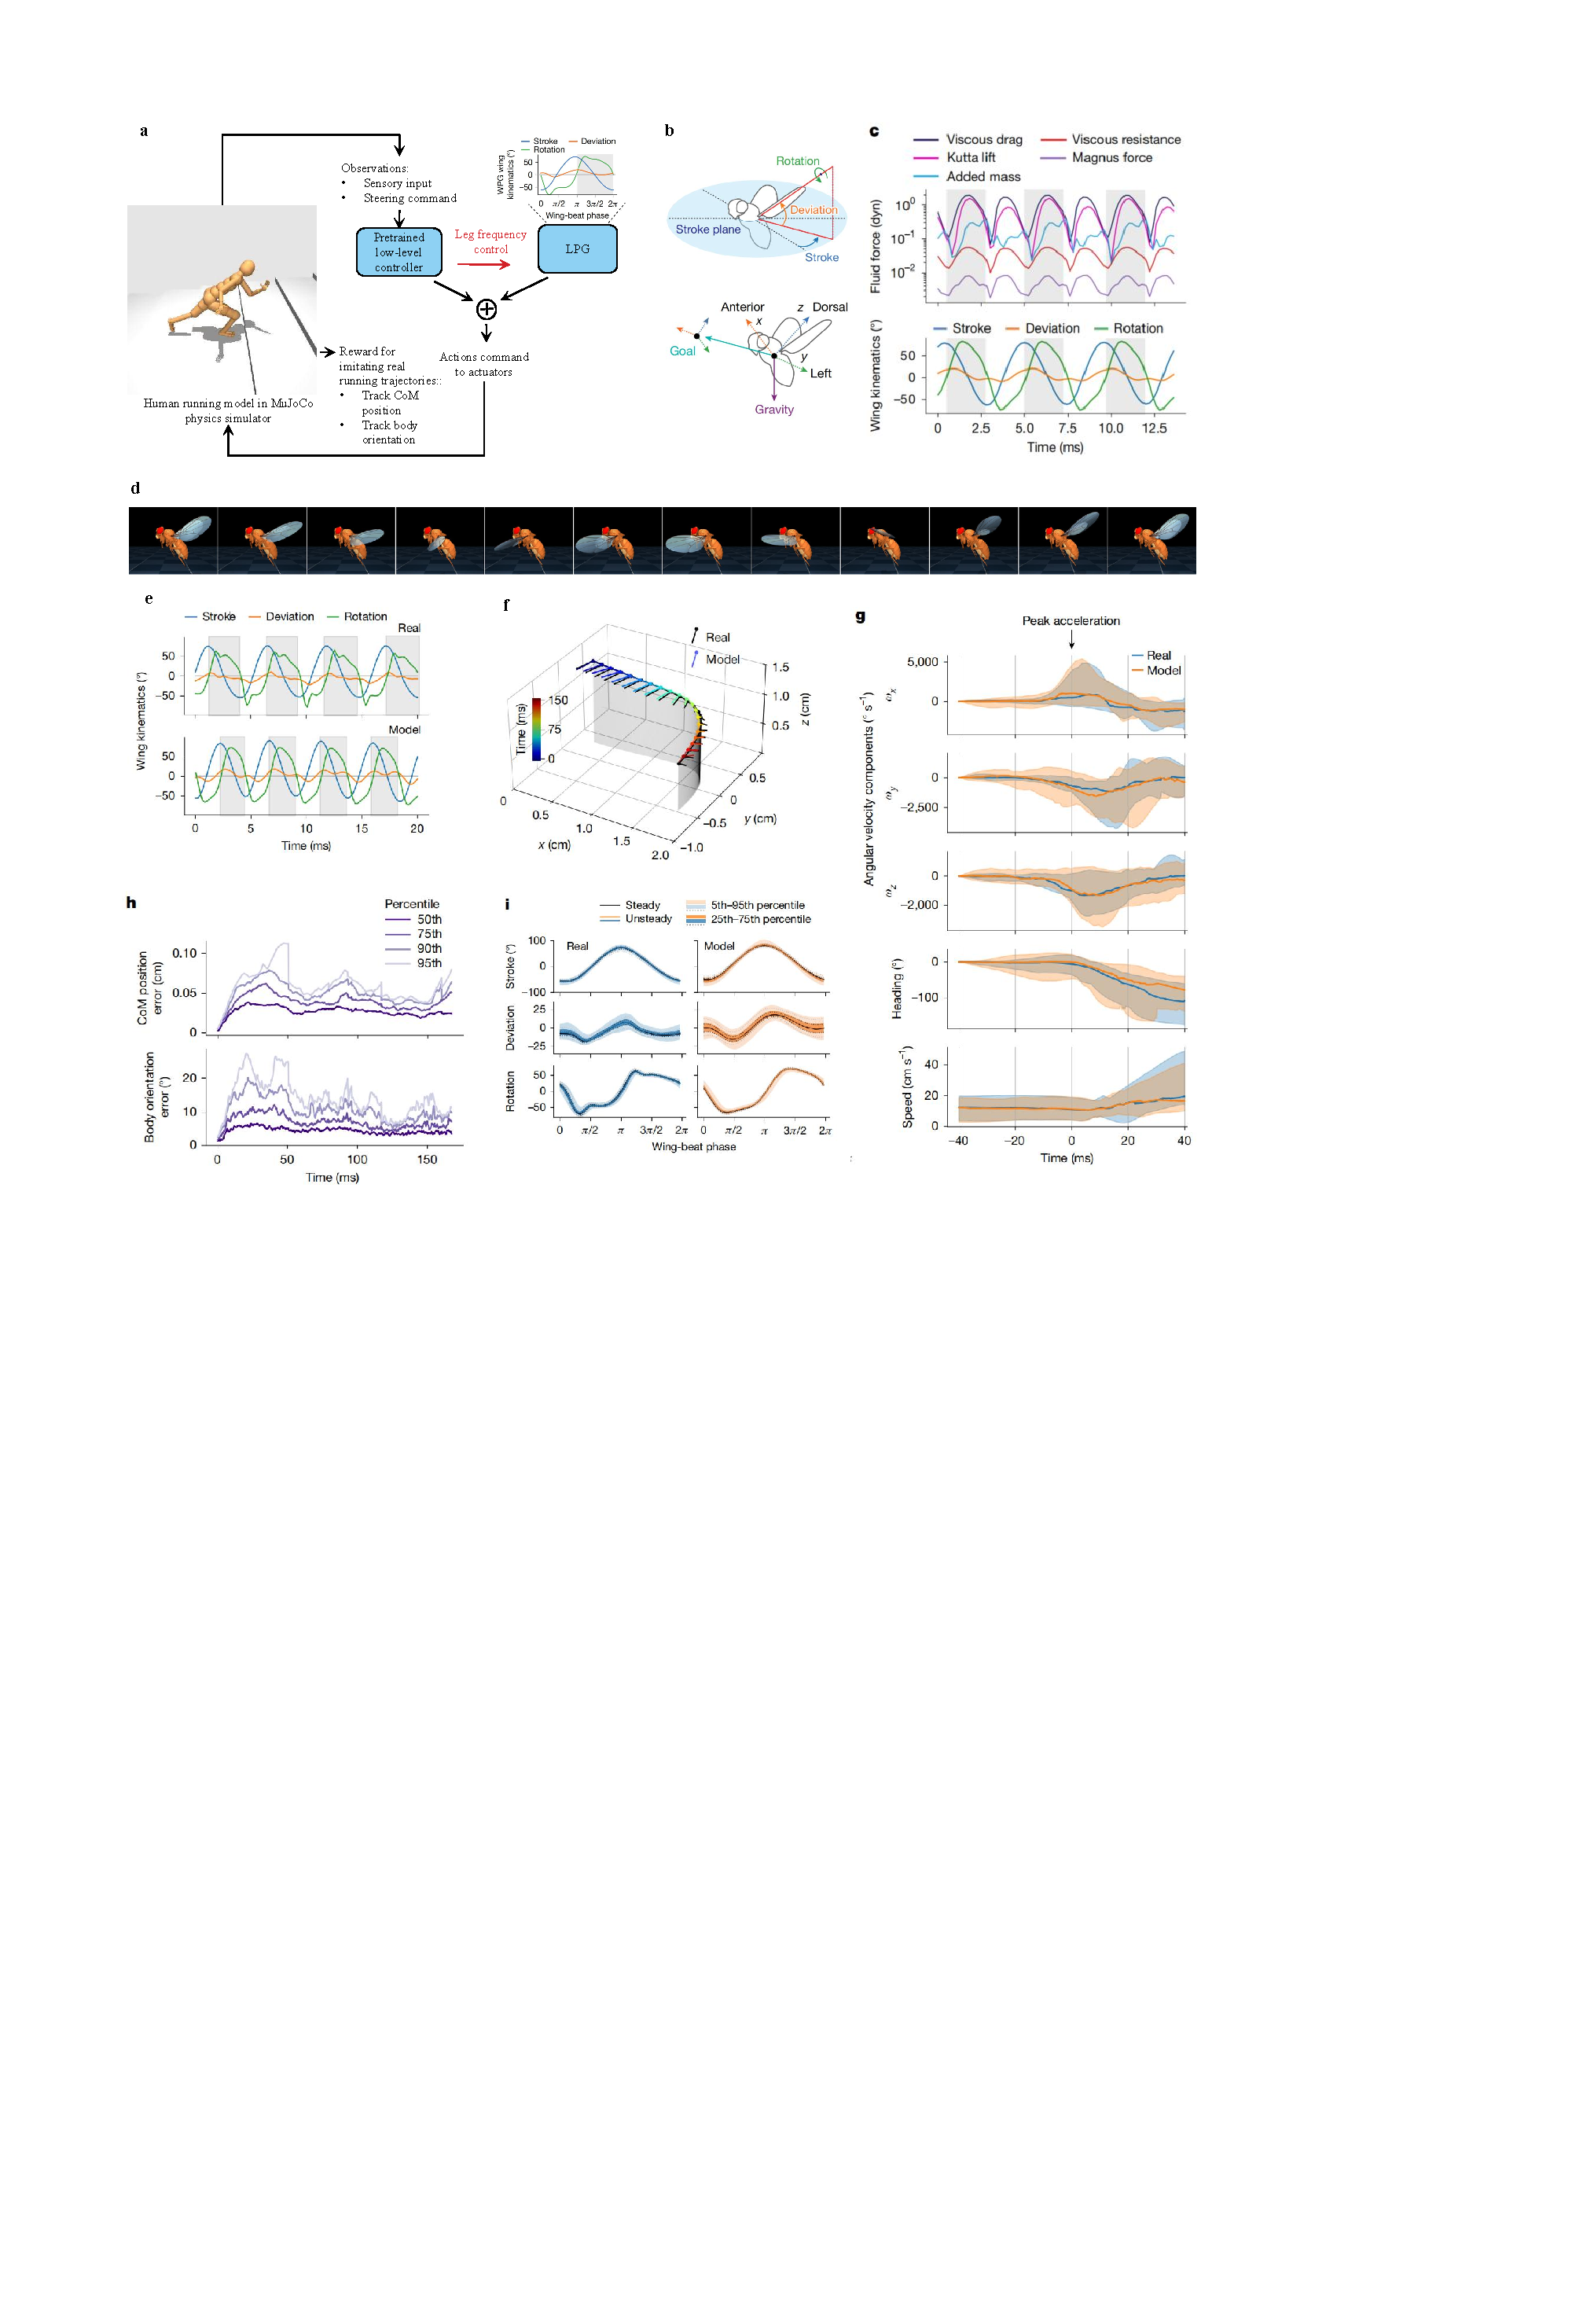
\includegraphics[width=0.9\textwidth]{fig/fig_3.pdf}
	\caption{
	} \label{fig:3}
\end{figure}


Geometric eigenmodes of the cortex are obtained by solving the eigenvalue problem of the LBO, which is also known as the Helmholtz equation (equation (\ref{eq:1})). 
In physically continuous systems, the solutions of the Helmholtz equation correspond to the spatial projections of the solutions of a more general wave equation, such that the resulting eigenmodes inherently represent the vibrational patterns, or standing waves, of the system’s dynamics\cite{levy2006laplace}. 
This equivalence implies that the superior efficacy of geometric eigenmodes in the reconstruction of diverse patterns of brain activity results from a fundamental role of wave dynamics in shaping these patterns, as predicted by NFT. 
This prediction has been confirmed through models of EEG recordings21,35, but waves across the whole brain have only recently been observed in fMRI signals\cite{robinson2005multiscale,bolt2022parsimonious} and thus far lack a theoretical explanation. 
Here we use NFT and geometric eigenmodes to show that wave dynamics can provide a unifying account of diverse empirical and physiological phenomena observed at scales accessible with fMRI.


We model neural activity using an isotropic damped NFT wave equation without regeneration\cite{robinson1997propagation} (Fig.~\ref{fig:4}a~and NFT wave model in Methods~\ref{sec:NFT_model}). 
Under this model, activity propagates between points on the neocortex through their white-matter connectivity with a strength that decays approximately exponentially with distance (Supplementary Fig.~\ref{fig:extended_fig_10}~and Supplementary Information~\ref{sec:NFT}~and~\ref{sec:NFT_wave}). 
To simulate resting-state neural activity we use a white noise input to mimic unstructured stochastic fluctuations\cite{robinson2005multiscale} (Modelling resting-state dynamics in Methods~\ref{sec:modelling_resting}). 
We compare the performance of this simple wave model with a biophysically based neural mass model (balanced excitation–inhibition (BEI) model) that has been used extensively to understand resting-state fMRI signals\cite{deco2014local} (Fig.~\ref{fig:4}a~and Neural mass model in Methods~\ref{sec:neural_mass}). 
The neural mass model is closely aligned with the classical, connectome-centric view of brain function, representing dynamics as the result of interactions between neuronal populations in discrete anatomical regions, coupled according to an empirically measured connectome.


We first compare the efficacy of the two models in capturing distinct and commonly studied properties of spontaneous, task-free FC: namely, static pairwise FC (edge FC), static node-level average FC (node FC) and time-resolved dynamic properties of FC (FCD) (Modelling resting-state dynamics in Methods~\ref{sec:modelling_resting}). 
Across all FC-based benchmark measures, the wave model shows comparable or superior performance in reconstruction of empirical data relative to the neural mass model (Fig.~\ref{fig:4}b). 
The wave model also captures time-lagged properties\cite{raut2021global,bolt2022parsimonious,mitra2015lag} of empirical resting-state activity more accurately than the mass model (Extended Data Fig.~\ref{fig:extended_fig_9}~and Measuring time-lagged properties of resting-state dynamics in Methods~\ref{sec:dynamics_measurement}). 
This strong performance of the wave model is remarkable given its relative simplicity: the wave model only requires the geometry of the cortex (that is, the surface mesh) as input and includes one fixed parameter and one free parameter ($ r_s $) for fitting to data (Extended Data Fig.~\ref{fig:extended_fig_10}) whereas the neural mass model requires a dMRI-derived interregional anatomical connectivity matrix and comprises 15 fixed parameters and four free parameters (Supplementary Information~\ref{sec:mass_optimization}). 
These considerations indicate that wave dynamics offer a more accurate and parsimonious mechanistic account of macroscale, spontaneous cortical dynamics captured by fMRI.


We next consider stimulus-evoked cortical activity in the wave model. 
We analyse cortical responses to sensory stimulation of primary visual cortex (V1), because it elicits a well-defined hierarchy of regional cortical responses\cite{felleman1991distributed,chaudhuri2015large} (Modelling stimulus-evoked dynamics in Methods). 
A 1 ms pulse input to V1 yields a propagating wave of activity that rapidly splits along the dorsal and ventral visual processing streams (Fig.~\ref{fig:4}c (arrows) and Supplementary Video 1), consistent with the mainstream understanding of hierarchical visual processing\cite{goodale1992separate}. 
Remarkably, this result indicates that geometric constraints on travelling waves of evoked activity are sufficient for the segregation of the dorsal and ventral processing streams, which have traditionally been thought to be driven primarily by complex patterns of layer-specific connectivity\cite{felleman1991distributed,goodale1992separate,markov2014anatomy}. 
Furthermore, the temporal profile of evoked responses across the visual system follows a well-defined timescale hierarchy, with higher-order association areas showing peak responses that are delayed and prolonged compared with lower-order visual areas (Fig.~\ref{fig:4}d). 
These findings thus indicate that this hierarchical ordering, previously identified in experimental and modelling studies\cite{chaudhuri2015large,hasson2008hierarchy,murray2014hierarchy}, emerges naturally from waves of excitation propagating through the cortical medium. Critically, this hierarchical temporal ordering of areal responses strongly correlates with an independent anatomical measure of the cortical processing hierarchy based on non-invasive estimates of myeloarchitecture (T1-weighted (T1w) and T2-weighted (T2w) ratio)\cite{glasser2011mapping,gao2020neuronal}. 
This correlation is particularly strong within the visual processing hierarchy ($ r = -0.72 $, one-sided spin-test $ P $ value ($P_{spin}$) = 0.003; Fig.~\ref{fig:4}e) but is also present when considering all cortical areas ($ r = -0.44 $, $ P_{spin} = 0.037 $; Supplementary Fig.~\ref{fig:supp_11}). 
Together, our modelling results show how simple wave dynamics unfolding on the geometry of the cortex provide a unifying generative mechanism for capturing complex properties of spatiotemporal brain activity.


\subsubsection{Geometry constrains subcortical activity}
\begin{figure}[!htb]
	\centering
	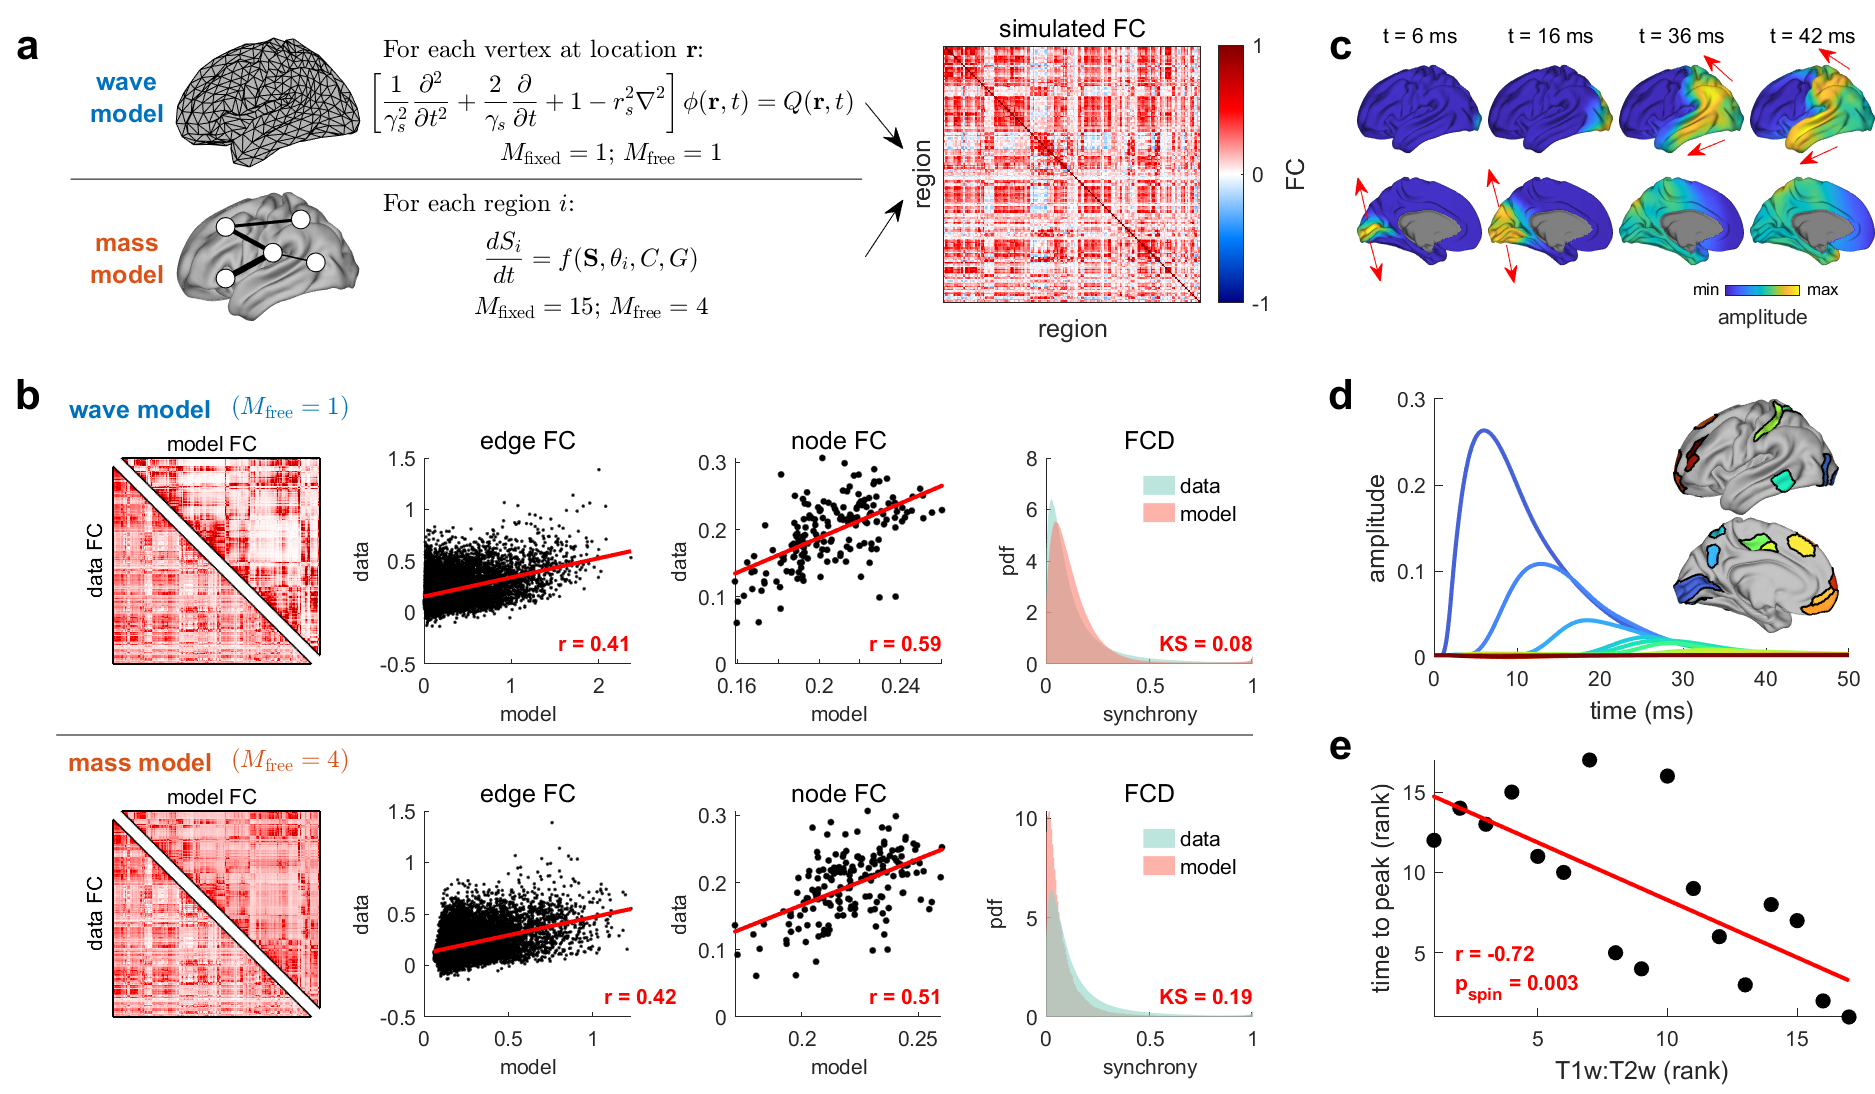
\includegraphics[width=0.9\textwidth]{fig/fig_4.pdf}
	\caption{
	} \label{fig:4}
\end{figure}


Our analyses thus far have focused on the strong coupling of geometry and dynamics in the neocortex. 
We next investigate this coupling in non-neocortical areas, focusing on the thalamus, striatum and hippocampus, because these structures have geometries easily captured using MRI data and their functional organization has been extensively studied\cite{tian2020topographic}.


We first generalize our eigenmode analysis to three-dimensional (3D) volumes (Estimating the geometric eigenmodes of non-neocortical structures in Methods), yielding geometric eigenmodes that extend spatially through the three spatial dimensions of each structure. 
Next, to fully capture the macroscale functional organization of these non-neocortical regions, we apply a widely used manifold learning procedure to voxel-wise FC data to obtain the key functional gradients in each structure\cite{haak2018connectopic} (Mapping the functional organization of non-neocortical structures in Methods). 
These functional gradients describe the principal axes of spatial organization dictated by similarities in FC, thus representing the dominant modes of variation in functional organization, ordered according to the percentage of variance in FC similarity that they explain.


The spatial profiles of the first three functional gradients of the thalamus, striatum and hippocampus (accounting for 24, 50 and 47\% of the variance in FC similarity, respectively) show a near-perfect match to the first three geometric eigenmodes (Fig.~\ref{fig:5}a–c; spatial correlations $ r\geq0.93 $). 
This tight correspondence generalizes out to the first 20 modes and first 20 gradients of each structure (with the first 20 gradients respectively accounting for 49, 70 and 68\% of total variance in FC similarity), with all absolute spatial correlations $ |r| > 0.5 $, except for the 20th gradient and 20th mode in the striatum and hippocampus (Fig.~\ref{fig:5}d–f). 
This strong relationship is striking given that the functional gradients are generated via a complex processing pipeline applied to fMRI-derived FC measures whereas the eigenmodes are derived simply from each structure’s geometry, independent of the functional data. These findings suggest that the functional organization of non-neocortical structures derives directly from their geometric eigenmodes.


\begin{figure}[!htb]
	\centering
	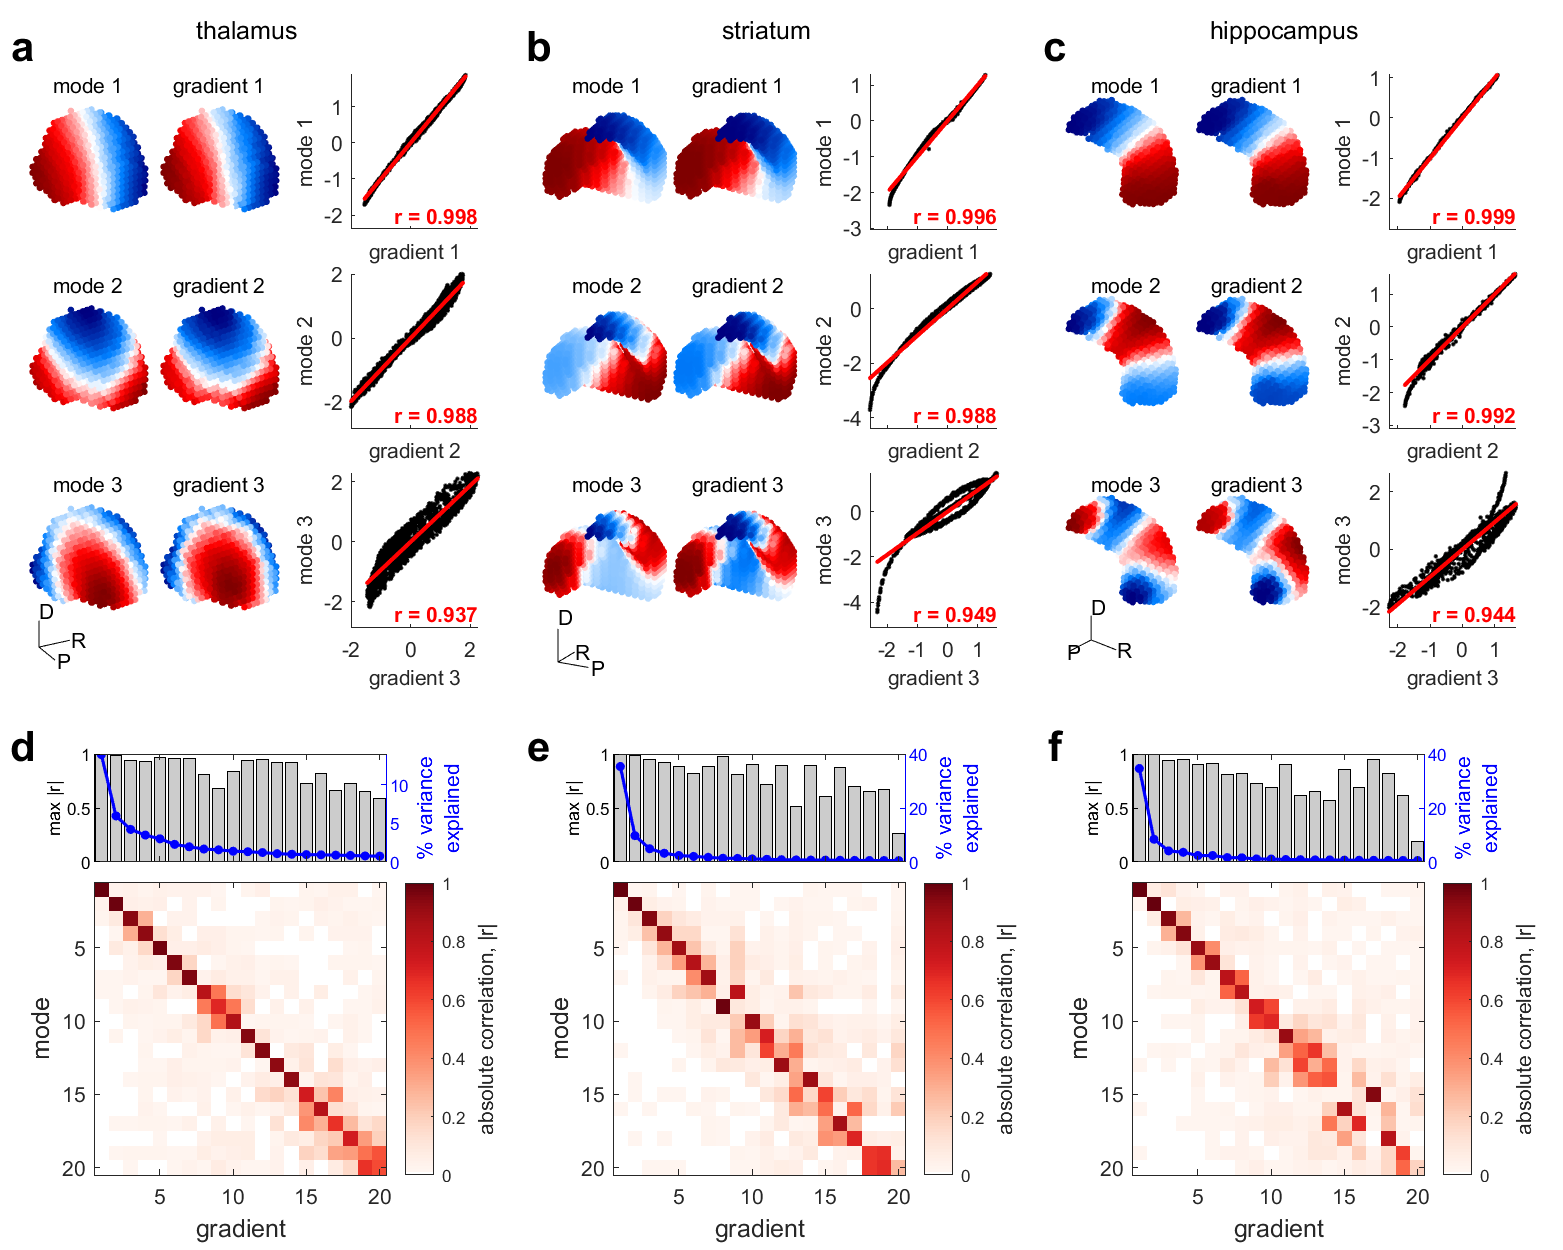
\includegraphics[width=0.9\textwidth]{fig/fig_5.pdf}
	\caption{
	} \label{fig:5}
\end{figure}



%\subsection{Detection of face images using the responses of face-selective units}
%
%\begin{figure}[!htb]
%	\centering
%	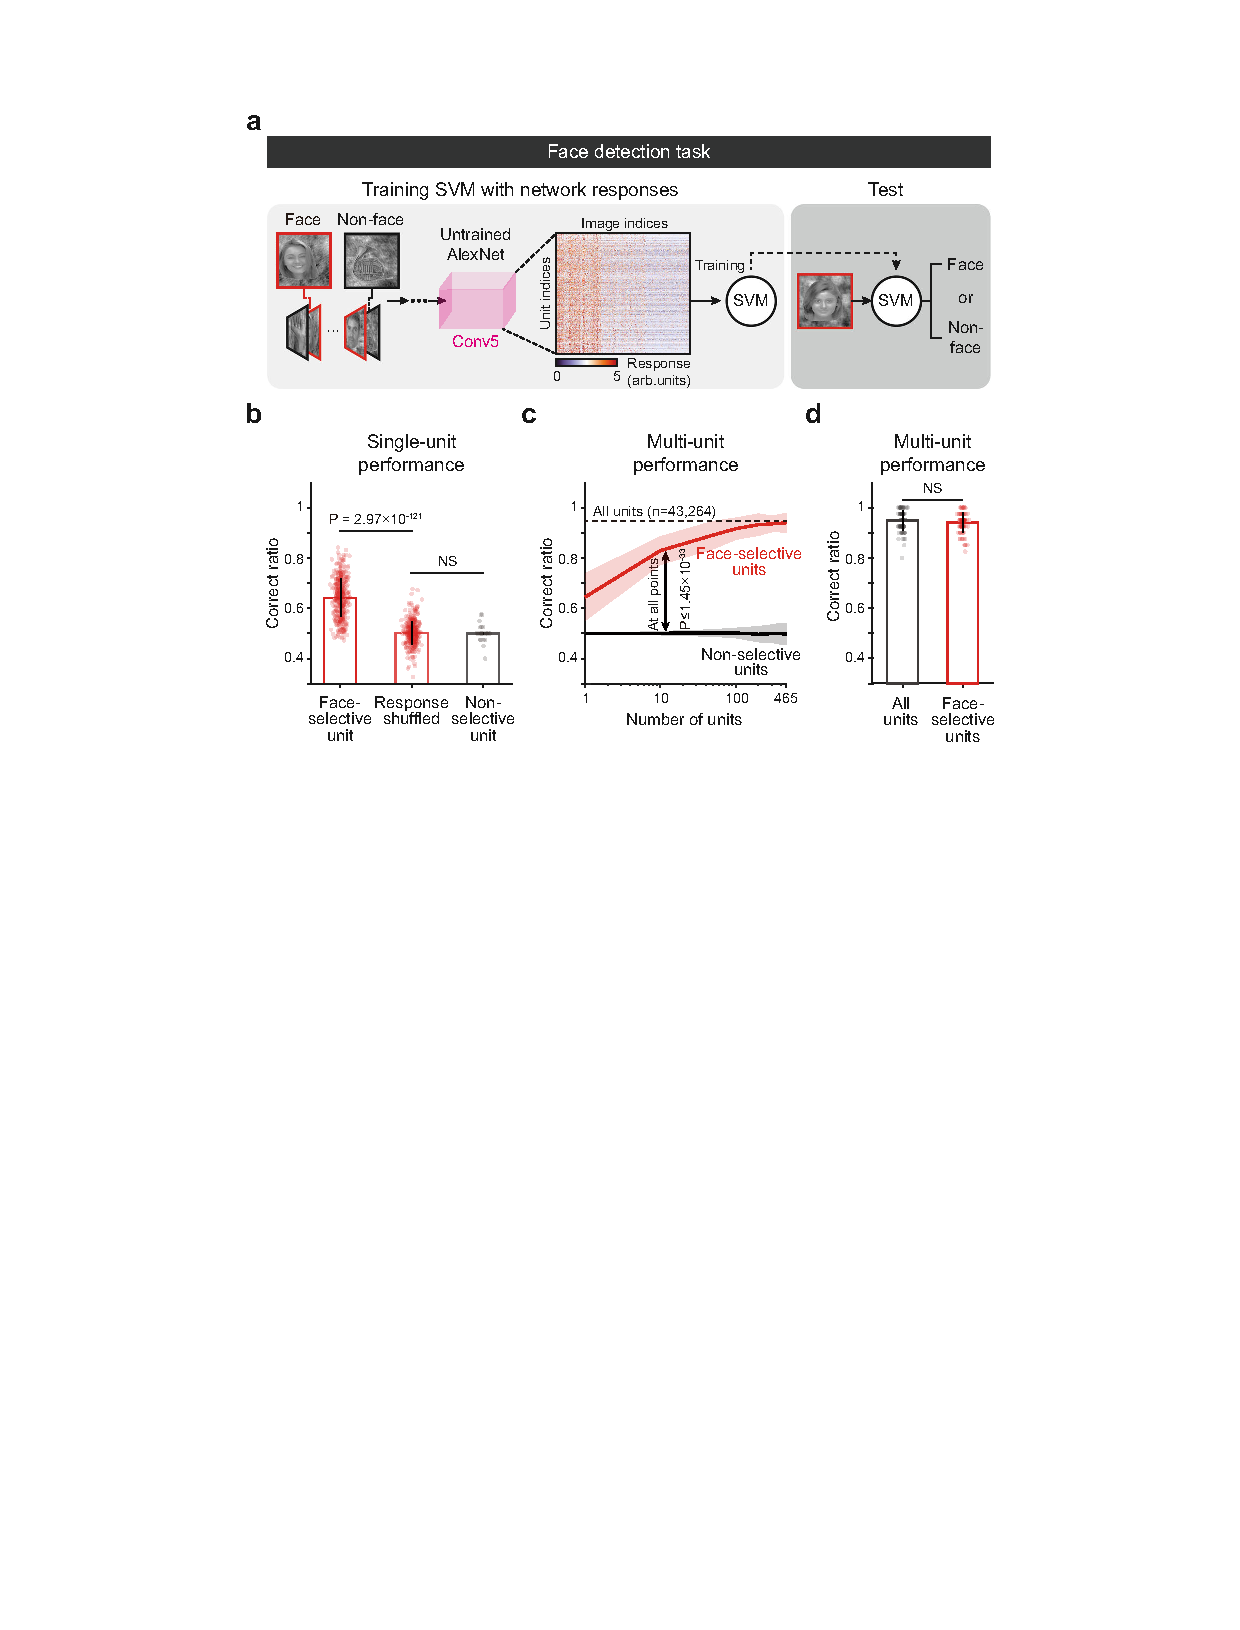
\includegraphics[width=0.9\textwidth]{fig/face_3.pdf}
%	\caption{
%		\textbf{Detection of face images using the response of face units in untrained networks.
%		}
%		(\textbf{a}) Design of the face detection task and SVM classifier using the responses of the untrained AlexNet.
%		During this task, face or non-face images were randomly presented to the networks and the observed response of the final layer was use d to train a support vector machine (SVM) to classify whether the given image was a face or not.
%		Among 60 images from each class (face, hand, horn, flower, chair, and scrambled face) that were not used for face unit selection, 40 images were randomly sampled for the training of the SVM, and the other 20 images were used for testing.
%		The images shown are selected examples from the publicly available dataset~\cite{stigliani2015temporal}.
%		The original images are available at [\url{http://vpnl.standford.edu/fLoc}].
%		(\textbf{b}) Performance on the face detection task using a single unit randomly sampled from face-selective units ($ n = 465 $) and units without selective responses to any image classes ($ n = 7776 $).
%		The channel level was measured by the shuffled responses of face-selective units in the untrained network.
%		The error bar indicates the standard deviation of each unit.
%		Each bar indicates the mean and the error bar indicates the standard deviation of performance of each unit.
%		(\textbf{c}) Performance of the face detection task using face-selective units and non-selective units when varying the number of units from 1 to 456.
%		The dashed line indicates the detection performance using all units in Conv5 ($ n=43,264 $).
%		Each line indicates the mean and the shaded area indicates the standard deviation for 100 repeated trials of the random sampling of units.
%		(\textbf{d}) Performance on the face detection task using face-selective units ($ n=465 $) and then using all units in Conv5 ($ n=43,264 $).
%		Each bar indicates the mean and the error bar indicates the standard deviation for 100 repeated trials of the random sampling of units.
%	} \label{fig:detection}
%\end{figure}
%
%
%We tested whether the selective responses of these face units could provide reliable information with which to detect between faces and non-face objects.
%During this task, face ($ n=40 $) or non-face ($ n=40 $) images were randomly presented to the networks, and the observed response of the final layer was used to train a support vector machine (SVM) to classify whether the given image was a face or not (\ref{fig:detection}a).
%First, we compared the detection performance of the SVM using a single unit randomly sampled from face-selective units and using units without selective responses to any image classes.
%We confirmed that the SVM trained with a single face-selective unit shows noticeably higher performance that those measured from shuffled responses, whereas the SVM trained with units without selectivity does not 
%(\ref{fig:detection}b,
%Face unit vs. Response shuffled, 
%$ n_\textrm{face} = 465 $,
%two-sided rank-sum test,
%$ P = 2.97 \times 10 ^{-121} $,
%$ r_{rbc} = 7.68 \times 10^{-1} $;
%Response shuffled vs. Non-selective unit, 
%$ n_\textrm{non-selective} = 7,776 $,
%two-sided rank-sum test, NS, 
%$ P = 1.10 \times 10^{-1} $,
%$ r_{rbc} = 4.52 \times 10^{-2} $,
%two-sided Kolmogorov-Smirnov test,
%$ P = 1.93 \times 10^{-1} $,
%$ d = 2.12 \times 10^{-2} $
%).
%Then, extending the test to various numbers of units, we compared the detection performance of this SVM using face-selective units with the performance when using the same number of randomly sampled non-selective units.
%We confirmed that the SVM trained with multiple face-selective units shows noticeably better performance that that trained with the same number of non-selective units, 
%as the number of units used in each condition was varied from $ n=1 $ to 465 (total number of face units in untrained networks)
%(\ref{fig:detection}c,
%Face vs. Non-selective units, 
%$ n_\textrm{trial} = 100 $,
%two-sided rank-sum test, 
%$ P \leq 1.45 \times 10^{-33} $,
%$ r_{rbc} \geq 8.74 \times 10^{-1} $
%).
%We also found that the SVM using face units ($ n=465 $) nearly matches the performance of the SVM using all units in the final layer ($ n=43,264 $)
%(\ref{fig:detection}d, 
%Face vs. All units, 
%$ n_\textrm{trial} = 100 $,
%two-sided rank-sum test, NS, 
%$ P = 1.90 \times 10^{-1} $,
%$ r_{rbc} = 9.29 \times 10^{-2} $,
%two-sided Kolmogorov-Smirnov test,
%$ P = 1.90 \times 10^{-1} $,
%$ d = 9.20 \times 10^{-3} $
%).
%Furthermore, we found that face units enable the networks to detect faces with various sizes, position, and rotations even when such image conditions were held constant when training the SVM classifier.
%
%
%Notably, we also found that the SVM can successfully detect faces when it is trained with the responses of units selective to non-face classes, 
%similar to the results in a previous experiment in human~\cite{haxby2001distributed},
%whereas it failed to detect with units not selective to any of the classes.
%To compare our results with the experiment condition of the previous human experiment~\cite{haxby2001distributed},
%we first trained the SVM using the responses of four distinct populations:
%(1) all of the units selective to each class (All-selective),
%(2) units selective to non-face classes (Non-face-selective),
%(3) face-selective units only (Face-selective),
%and (4) units not selective to any of the classes (Non-selective).
%As a result, we found that the SVM trained with non-face-selective units showed a performance comparable with the results of Haxby et al.~\cite{haxby2001distributed}.
%Interestingly, the performance was also comparable with those with all-selective units and those with face-selective units only,
%similar to the results in a previous experiment in human~\cite{haxby2001distributed}.
%This result is understandable considering that there are only five image classes;
%thus, even non-face-selective units can provide information for discriminating face and non-face images by generating different levels of activities for each class.
%Taken together, these results imply that the information provided by selective units that emerge in the untrained networks is sufficient to detect between faces and non-face objects.
%
%
%%\subsection{The emergence of face-selectivity in trained DNNs}
%
%
%\begin{figure}[!htb]
%	\centering
%	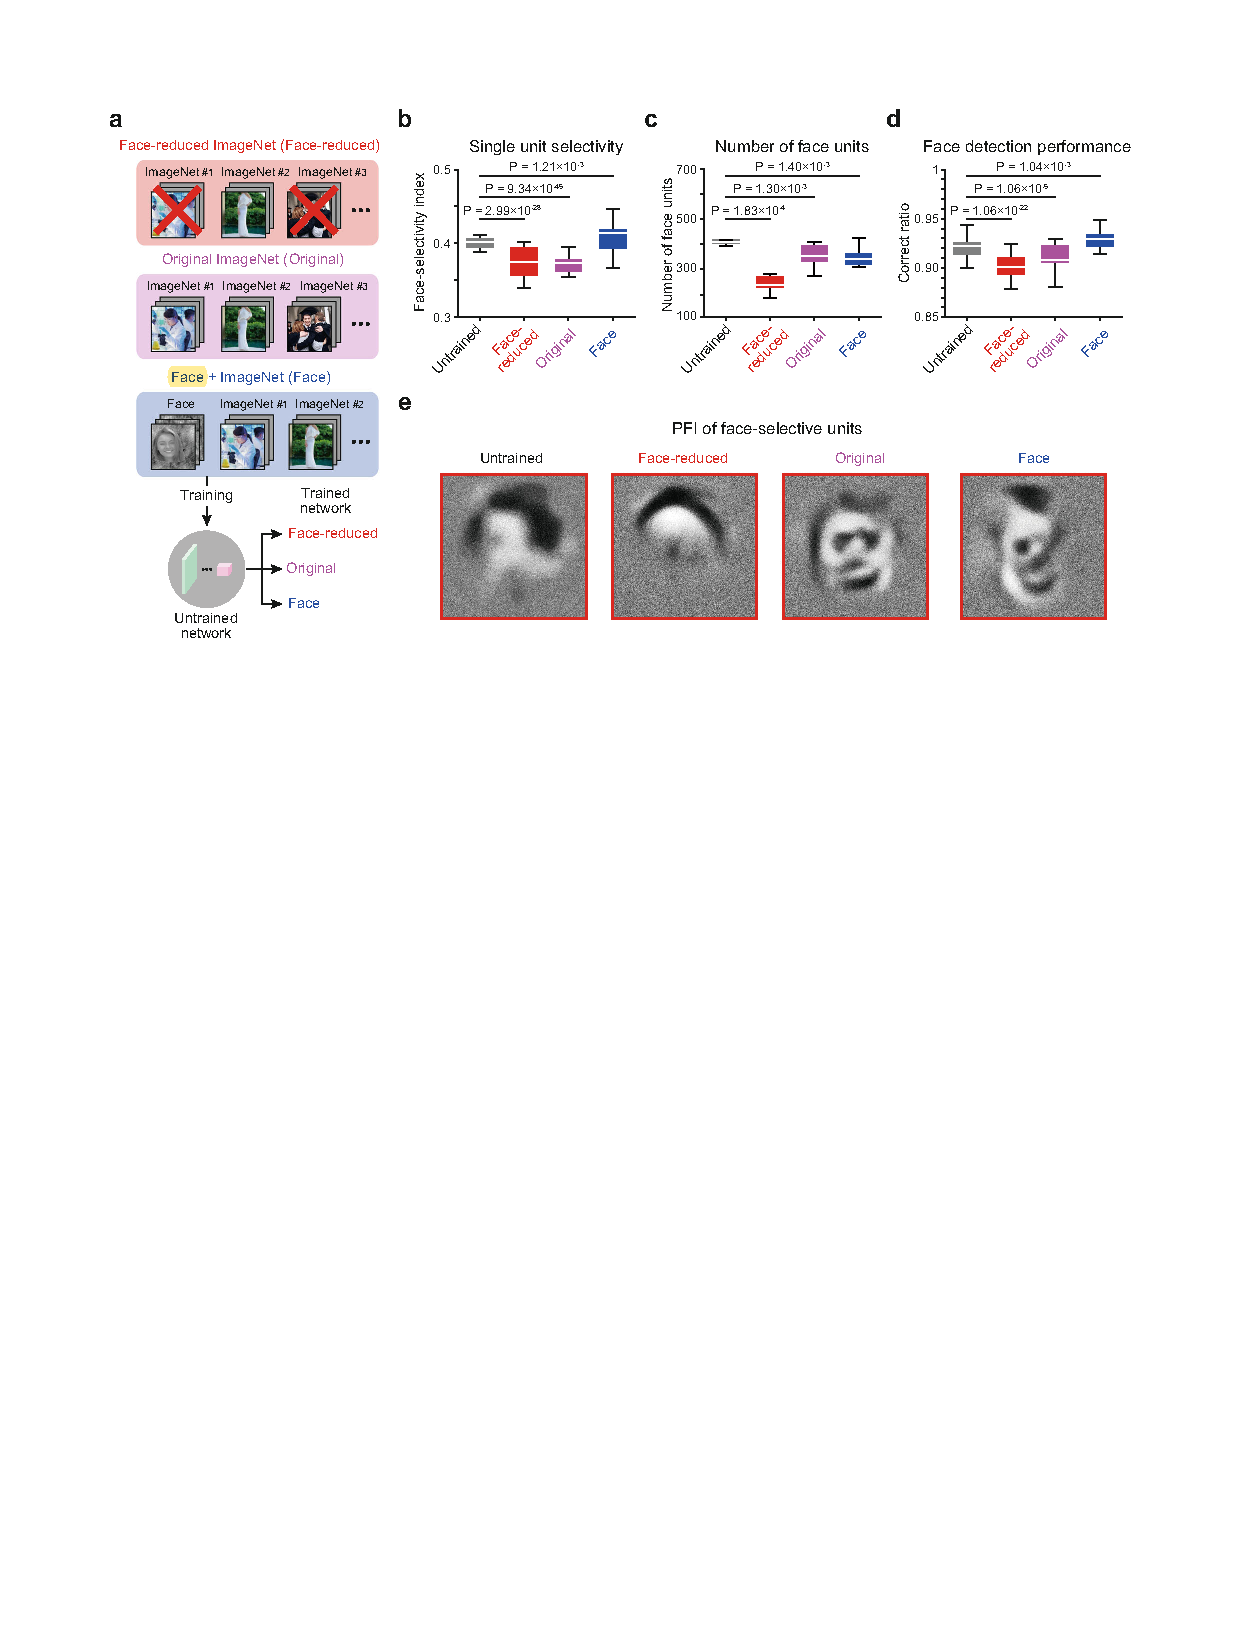
\includegraphics[width=1.0\textwidth]{fig/face_4.pdf}
%	\caption{
%		\textbf{Effect of training on face-selectivity in untrained networks.
%		}
%		(\textbf{a}) Three different datasets modified from publicly available ImageNet~\cite{ILSVRC15} were used for the training of the network for image classification: 
%		(1) face-reduced ImageNet, 
%		(2) original Imagenet, 
%		and (3) ImageNet with added face images.
%		For copyright reasons, the face image shown here is not the actual image used in the experiments.
%		The original images are replaced with images with similar contents for display purposes.
%		The original images are available at [\url{https://www.image-net.org/download}].
%		Images shown are available at [\url{https://www.shutterstock.com},\url{http://vpnl.stanford.edu/fLoc/}~\cite{stigliani2015temporal}].
%		(\textbf{b}) Face-selectivity index of face-selective units in untrained network and in networks trained with the three datasets ($ n_\textrm{Untrained} = 4,267 $, $ n_\textrm{Reduced} = 2,452 $, $ n_\textrm{Original} = 3,561 $, $ n_\textrm{Face} = 3,585 $).
%		(\textbf{c}) The number of face-selective units in untrained networks and in networks trained with three datasets ($ n_\text{net} = 10 $).
%		(\textbf{d}) Face detection performance of untrained networks and of networks trained with three different datasets ($ n_\textrm{trial} = 1,000 $).
%		(\textbf{e}) The obtained preferred feature images (PFI), using reverse-correlation method of the face-selective unit on each network.
%		All box plots indicate the inter-quartile range (IQR between Q1 and Q3) of the dataset,
%		the horizontal line depicts the median and the whiskers correspond to the rest of the distribution (Q1-1.5*IQR, Q3+1.5*IQR).
%	} \label{fig:effect}
%\end{figure}
%
%
%We tested a scenario in which our current model can corroborate the conflicting observations regarding the role of visual experience for the development of face-selectivity.
%A previous report suggested that visual experience is necessary for the emergence of face-selectivity by showing that monkeys raised without exposure to faces lack face-selective domains~\cite{arcaro2017seeing}.
%On the other hand, another recent study showed that the face-selective area develops robustly in congenitally blind humans, suggesting that visual experience is not necessary for face-selectivity~\cite{arcaro2017seeing}.
%Regarding these conflicting results, we examined how face-selective units in untrained networks can be affected by training with visual inputs.
%
%
%To investigate the effect of training on a face image set,
%we prepared the following three different stimulus sets:
%(1) face-reduced ImageNet: 500 classes including no recognizable face images were manually curated from the ILSVRC 2010 dataset according to a visual inspection by the authors,
%(2) the original ImageNet, 
%and (3) the original ImageNet with added face images used in the current study~\ref{fig:effect}a.
%Then, the network was trained with each of these image sets.
%First, we found that the FSI of the face-selective units was significantly decreased after being trained to the face-reduced image set 
%(~\ref{fig:effect}b,
%Untrained vs. Face-reduced,
%$ n_\textrm{Untrained} = 4,267 $,
%$ n_\textrm{Reduced} = 2,452 $,
%two-sided rank-sum test,
%$ P = 2.99 \times 10^{-28} $,
%$ r_\textrm{rbc} = 6.76 \times 10^{-1} $
%),
%whereas it was increased after being trained to the face-including image sets 
%(Untrained vs. Face-included,
%$ n_\textrm{Face} =3585 $,
%two-sided rank-sum test,
%$ P = 1.21 \times 10^{-3} $,
%$ r_{rbc} = 2.60 \times 10^{-1} $
%).
%Notable, the FSI was significantly decreased after being trained to the original ImageNet dataset that contains images of faces but has no group labeled as face
%(~\ref{fig:effect}b, Untrained vs. Original, 
%$ n_\textrm{Original} = 3,561 $,
%two-sided rank-sum test,
%$ P = 9.34 \times 10^{-45} $,
%$ r_\textrm{rbc} = 8.15 \times 10^{-1} $
%).
%This suggests that the tuning of face-selective units could either be sharpened or weakened by training with distinct stimulus sets.
%
%% Fig.4 c
%Next, we found that the number of face-selective units observed was greater in the network trained with face-including image set compared to that trained to face-reduced images 
%(\ref{fig:effect}c, Untrained vs. Trained,
%$ n_\textrm{Net} = 10 $,
%two-sided rank-sum test,
%$ P \leq 1.40 \times 10 ^{-3} $,
%$ r_\textrm{rbc} \geq 5.72 \times 10^{-1} $
%).
%Interesting, however, we found that the number of face-selective units, when trained to face-including images, appeared to be smaller than that of untrained networks.
%These results imply that the training process of the network to face-including images selectively sharpens the tuning of face units so that the selectivity of strongly tuned units is sharpened while the weakly tuned units are pruned.
%In this condition, the face detection performance of the networks would improve in face-trained networks even if the number of face units decreased compared to the initial, untrained condition.
%To validate this scenario, we trained the SVM using the response of face-selective units for a face detection task in an untrained network and in the three networks trained to each type of data set.
%As predicted, we found that the face detection performance was significantly increased in the networks trained to the face-including image set compared to that of the untrained network
%(~\ref{fig:effect}d, Untrained vs. Face included, 
%$ n_\textrm{trial} = 1000 $,
%two-sided rank-sum test,
%$ P = 1.04 \times 10^{-3} $,
%$ r_\textrm{rbc} = 2.60 \times 10^{-1} $
%),
%whereas the face detection performance of the network trained to the face-reduced image set was significantly decreased compared to the untrained network
%(~\ref{fig:effect}, Untrained vs. Face-reduced,
%$ n_\textrm{trial} = 1,000 $,
%two-sided rank-sum test,
%$ P = 1.06 \times 10^{-22} $,
%$ r_\textrm{rbc} = 6.42 \times 10^{-1} $
%).
%Furthermore, we found that the PFI of the face-selective unit shows a clear face configuration in the network trained to face-including natural images,
%whereas the face configuration is disrupted in network trained to face-reduced dataset (\ref{fig:effect}e).
%This result is consistent with previous observation of decreased face-selectivity in face-deprived monkeys~\cite{arcaro2017seeing}.





\section{Discussion}

\section{Method} \label{sec:method}

% 使用贝叶斯优化或神经架构搜索找类别选择网络
\subsection{Neural architecture search}

\subsection{Derivation of cortical geometric eigenmodes} \label{sec:derivation}


\begin{equation}\label{eq:surface_curvature}
	\Delta:=\frac{1}{W} \sum_{i,j} \frac{\partial}{\partial x_i} (g^{ij} W \frac{\partial}{\partial x_j})
\end{equation}


\begin{equation}
	\text{wavelength} = \frac{2 \pi R_s}
	{\sqrt{l(l+1)}},
\end{equation}


\subsection{Modal decomposition of brain activity} \label{sec:modal_decomposition}


\begin{equation}\label{eq:weighted_sum}
	y(\textbf{r}, t) = \sum_{j=1}^{N} a_j(t) \psi_j(\textbf{r}),
\end{equation}


\begin{equation}\label{eq:amplitudes}
	a_j(t) = \int y(\textbf{r}, t) \psi_j(\textbf{r}) d\textbf{r}, 
\end{equation}


\subsection{HCP data} \label{sec:HCP_data}


\subsection{Cortical parcellations} \label{sec:cortical_parcellations}


\subsection{Derivation of connectome eigenmodes} \label{sec:connectome_derivation}

\begin{equation}\label{eq:connectome_eigenmodes}
	L' \psi = - \lambda \psi,
\end{equation}


\begin{equation}\label{eq:unnormalized_Laplacian}
	L = \frac{1}{2} [ (D-A_C) + (D-A_C)^T ],
\end{equation}


\subsection{Derivation of EDR eigenmodes} \label{sec:EDR_derivation}


\subsection{Comparisons with statistical basis sets} \label{sec:sets_comparisons}


\subsection{Modal power spectra of task-evoked activation maps} \label{sec:modal_power}


\begin{equation}\label{eq:normalized_power}
	P_j = \frac{|a_j|^2}{\sum_{j=1}^{N} |a_j|^2 }.
\end{equation}


\subsection{Contributions of long- and short-wavelength modes} \label{sec:wavelength_contributions}


\subsection{NFT wave model} \label{sec:NFT_model}


\begin{equation}\label{eq:NFT_wave_model}
	[\frac{1}{\gamma_s^2} \frac{\partial ^2}{\partial t^2} + 
	\frac{2}{\gamma_s} \frac{\partial}{\partial t} + 1 - r_s^2 \nabla^2] 
	\phi(\textbf{r}, t) = Q(\textbf{r}, t),
\end{equation}


\subsection{Neural mass model} \label{sec:neural_mass} 


\begin{equation}\label{eq:temporal_activity}
	\frac{dS_i}{dt} = f(\boldsymbol{S}, \theta_i, C, G), 
\end{equation}


\begin{equation}\label{eq:synaptic_gating_E}
	\frac{dS_i^{(E)}}{dt} = - \frac{S_i^{(E)}}{\tau_E} + (1-S_i^{(E)} \gamma r_i^(E) + \sigma \mu_i(t)),
\end{equation}

\begin{equation}\label{eq:synaptic_gating_I}
	\frac{dS_i^{(I)}}{dt} = - \frac{S_i^{(I)}}{\tau_I} + r_i^{I} + \sigma \mu_i(t),
\end{equation}

\begin{equation}\label{eq:firing_rate_E}
	r_i^{E} = H^{(E)} (I_i^{(E)}) = \frac{a_E I_i^{(E)} - b_E}{1 - exp[-d_e (a_E I_i^{(E)} - b_E)]},
\end{equation}

\begin{equation}\label{eq:firing_rate_I}
	r_i^{(I)} = H^{I} (I_i^{I}) = \frac{a_I I_i^{(I)} - b_I}{1 - exp[-d_E (a_E I_i^{(E)}) - b_I]'},
\end{equation}

% Excitatory
\begin{equation}\label{eq:input_current_E}
	I_i^{(E)}(t) = I^{ext} + W_E I_0 + w_{EE} S_i^{(E)} (t) + G J \sum_j C_{ij} S_j^{(E)}(t) - w_{IE} S_i^{(I)} (t), 
\end{equation}

% Inhibition
\begin{equation}\label{eq:input_current_I}
	I_i^{I} (t) = W_I I_0 +
	W_{EI} S_i^{(E)} (t) - 
	S_i^{(I)} (t),
\end{equation}


\subsection{Haemodynamic model} \label{sec:haemodynamic_model}


\begin{equation}\label{eq:vasodilatory_signal}
	\frac{dz_i}{dt} = N_i (t) - 
	\kappa z_i(t) - 
	\gamma [f_i(t) - 1], 
\end{equation}


\begin{equation}\label{eq:blood_inflow}
	\frac{df_i}{dt} = z_i(t),
\end{equation}


\begin{equation}\label{eq:blood_volume}
	\frac{dv_i}{d_t} = \frac{1}{\tau} [f_i(t) - v_i^{1/\alpha} (t)],
\end{equation}


\begin{equation}\label{eq:deoxyhaemoglobin}
	\frac{dq_i}{dt} = \frac{1}{\tau}
	\{
	\frac{f_i(t)}{\rho}
	[1 - (1-\rho)^{1/f_i(t)}]
	- v_i^{1/\alpha - 1} (t)
	\},
\end{equation}


\begin{equation}\label{eq:BOLD_signal}
	\frac{dy_i}{dt} = V_0
	\{
	k_1 [1 - q_i(t)] +
	k_2 [1 - \frac{q_i(t)}{v_i(t)}] + 
	k_3 [1 - v_i(t)]
	\},
\end{equation}


\subsection{Modelling resting-state dynamics} \label{sec:modelling_resting}


\begin{equation}\label{eq:synchrony}
	\Delta(i,j,t) = cos [\theta_i (t) - \theta_j (t)].
\end{equation}


\begin{equation}\label{eq:synchrony_similarity}
	\phi_{uv} = \frac{1}{d_u d_v} 
	\sum_{i>j} \Delta(i,j,\tau_u) \Delta(i,j,\tau_v),
\end{equation}

\begin{equation}\label{key}
	d_x = \sqrt{\sum_{i>j}
		[
		\Delta(i,j,\tau_x)
		]^2
	}.
\end{equation}


\subsection{Measurement of time-lagged properties of resting-state dynamics} \label{sec:dynamics_measurement}






\subsection{Modelling stimulus-evoked dynamics} \label{sec:modelling_stimulus}


\subsection{Estimation of the geometric eigenmodes of non-neocortical structures} \label{sec:geometric_estimation}


\subsection{Mapping the functional organization of non-neocortical structures} \label{sec:functional_mapping}


\subsection{Neural network model} \label{sec:nn}
We used AlexNet~\cite{krizhevsky2012imagenet} as a representative model of the convolutional neural network.
This network consists of feature extraction and classification networks.
The feature extraction network consists of five convolutional layers with rectified linear unit (ReLU) activation and a pooling layer, while the classification network has three fully connected layers.
The detailed parameters of the architecture were sourced from Krizhevsky et al.~\cite{krizhevsky2012imagenet}, which provided the models for V4 and IT~\cite{cadieu2014deep}.


To determine the origin of face-selective neurons, the randomly initialized networks were examined.
% 节点数目的开方为标准差
For the untrained AlexNet, the weights and biases of each convolutional layer were initialized from a Gaussian distribution or a uniform distribution with a zero mean and the standard deviation set to the square root of one over the number of units in the previous layer.
This was done to balance the strength of the input signals across the layers, 
and this approach follows previous research on efficient network initialization processes~\cite{lecun2002efficient}.


\subsection{Stimulus dataset}
Seven types of visual stimuli from six datasets were used.
(1) A low-level feature-controlled stimulus set~\cite{stigliani2015temporal} was selected and modified from publicly available images in human fMRI study~\cite{stigliani2015temporal} (\url{http://vpnl.stanford.edu/fLoc}) 
and was used to find units that responded selectively to face images.
Specifically, 260 images were prepared for each class (face, hand, horn, flower, chair, and scrambled face).
Then, 200 images were randomly sampled from each class and used for face unit selection.
Among the 60 remaining images in each class, 40 images were used for the training of the SVM, 
and the other 20 images used for testing.
Each item was overlaid on a group of phase-scrambled background images.
This was designed to reduce inter-class differences across various low-level properties,
in this case, luminance, contrast, size, position, and the degree of intra-/inter-class image similarity.
% 2
To validate the face-selective response to novel face stimulus set, we used (2) 16 face images used in Tsao et al.~\cite{tsao2006cortical,freiwald2010functional} provide by D.Tsao group from personal communication,
% 3
(3) 50 face images from open access VGGFace2 dataset used in Cao et al.~\cite{cao2018vggface2} (\url{https://github.com/ox-vgg/vgg_face2});
% 4
(4) 50 face images artificially generated by the FaceGen simulator (singular inversions; FaceGen Modeller Pro) in color and grayscale (\url{https://facegen.com}).
% 5
(5) To investigate the invariance of face-selective units to face images of various sizes, position, and rotation angle of the faces and other objects in the similarity-controlled stimulus set~\cite{stigliani2015temporal}.
% 6
(6) Viewpoint dataset: This set was used to find units that invariantly responded to face images of different viewpoints.
This dataset consists of five angle-based viewpoint classes ($ -90^\circ $, $ -45^\circ $, $ 0^\circ $, $ 45^\circ $, $ 90^\circ $) with 10 different faces obtained from the publicly available Point'04 dataset (\url{http://crowley-coutaz.fr/Head%20Pose%	20Image%20Database.html}) used in Gourier et al~\cite{gourier2004estimating}.
% 7
To investigate the possibility of units selective to various objects, we used a publicly available ImageNet dataset~\cite{russakovsky2015imagenet} (\url{https://www.image-net.org/download}).
For copyright reasons, the images in ~\ref{fig:emergence}a, ~\ref{fig:effect}a, and ~\ref{fig:image_net}a,d are not the actual images used in our experiments.
The original images are replaced with images with similar contents for display purposes.
Alternative images used in this study are purchased from \url{https://www.shutterstock.com} with a standard image license, which includes rights to publish in e-publication and printed in physical form as part of a copy of magazines, newspapers, and books.
For all datasets, the image size of the input to AlexNet was fixed at $ 227 \times 227 $ pixels.


\subsection{Analysis of response of the network units}
In our model, a unit refers to a unit component at each position of the channel in an activation map of the network.
We defined this unit in a convolutional network as a simplified model of a biological unit (a single neuron or a group of neurons that generates a tuned activity), considering that the dynamics of a single neuron in biological brains can be estimated from its receptive filed, 
which behaves as a spatiotemporal filter at a local cortical position retinotopically matching the external visual space.
Based on a previous study~\cite{grossman2019convergent}, face-selective units were defined as units that had significantly higher mean responses to face images than to images in any non-face class ($ P \textless 0.001 $, two-sided rank-sum test).
To estimate the normalized response, the responses to each unit was $ z $-scored using the average and the standard deviation of responses to stimulus images.
To quantify the degree of tuning, an FSI of a single unit was defined as in previous experimental research~\cite{aparicio2016neurophysiological}
\begin{equation}\label{eq:fsi}
	FSI = \frac{(\overline{R}_\textrm{face} - \overline{R}_\textrm{non-face})}
	{\sqrt{(\sigma^2_\textrm{face} + \sigma^2_\textrm{non-face}) / 2}}
\end{equation}
where $ \overline{R}_\textrm{face} $ is the average response to face images 
and $ \overline{R}_\textrm{non-face} $ is the average response to all non-face images.
An FSI of 0 indicates equal responses to face and non-face objects.


Among the face-selective units found, a face viewpoint-invariant unit was defined as a unit for which the response was not significantly different (one-way ANOVA, $ P \textgreater 0.05 $, Bonferroni adjustment $ n = 5 $) among all viewpoint classes.
Similar to the face-selective units, the viewpoint-specific units were determined by the mean response of the preferred viewpoint class being significantly higher than that for any other viewpoint (one-way ANOVA, $ P \textless 0.05 $, Bonferroni adjustment $ n = 5 $).
We defined mirror-symmetric tuning as the condition that arises when a viewpoint-specific face-selective unit has a symmetric shape of the tuning curve (one-way ANOVA, $ P \textless 0.05 $, Bonferroni adjustment $ n = 5 $; i.e., a unit shows peak responses at $ -45^\circ $ and $ 45^\circ $ or $ -90^\circ $ and $ 90^\circ $).
The invariance index of a single unit was defined as the inverse of the standard deviation of the average responses for images within each viewpoint class.
The same analysis was also performed for the stimulus set that added the face class to ILSVRC2010.


\subsection{Face vs. non-face detection task for the network}
A face vs. non-face detection task was established to investigate whether face-selective units could perform basic face perception.
To determine if this was possible, an SVM was trained with network responses to images and was then made to predict whether a class of unseen images was or was not a face.
% 循环验证指以任何形式,回溯地选择数据的某个特征作为因变量进行分析,从而扭曲统计检验结果。
% 循环验证有很多种形式,但本质上都包含先使用数据刻画(characterize)某需要被检验的变量,然后再对该批数据进行分析并进行统计推断,因此通常被称为“双重浸渍”(double dipping)。
To avoid the double-dipping issue~\cite{kriegeskorte2009circular} we undertook the training and testing of the SVM using distinct sets of images, 
where 260 images were prepared for each class, 
and 200 image were then randomly sampled from those images and used for face unit selection.
Among the 60 remaining images in each class, 40 images were used for the training of the SVM, 
and the other 20 images were used for testing.
The label of the training set was then changed to a binary class: face or non-face.
For each trial, the SVM was trained with the relationship between the fifth layer's response to the training set and the new training label.
After a training session, the model predicted the test label using the network response to the test set.
Furthermore, to test whether the responses of face-selective units could detect faces varied in different ways, 
we trained an SVM with network responses for center-view face images ($ N = 40 $) and non-face images $ N = 40 $.
The model then predicted test labels using the responses of face-selective units to new test sets which consisted of a face and non-face images with different types of variation, in this case, different sizes, positions, and rotation angles.


\subsection{Preferred input feature (receptive field) analysis} \label{sec:preferred}
To visualize the preferred input feature of target units, the receptive field was estimated by the RC method~\cite{bonin2011local} with multiple iterations.
The initial stimulus set was generated as 2500 random local 2D Gaussian filters.
Such stimuli were weighted by the corresponding responses and were added as an initial preferred feature image.
Then, to detect the preferred feature more accurately, we calculated the PFI iteratively;
the PFI of the next iteration was calculated by a new stimulus set consisting of the summation of the current PFI and 2500 random local 2D Gaussian filters (\ref{fig:preferred}a).
We repeated 100 iterations and obtained the final PFI.


% b
To obtain the preferred feature images of target units, we used a generative adversarial network (X-Dream)~\cite{dosovitskiy2016generating}.
X-Dream consists of a generative adversarial network (GAN) with a genetic algorithm as the optimization algorithm of the responses.
We used a GAN~\cite{dosovitskiy2016generating} pre-trained with natural images (ILSVRC 2012).
The response optimization algorithm~\cite{ponce2019evolving} finds the optimal image code that maximizes the response of the target unit.
In this algorithm, a single image code consists of 1000 initial values randomly sampled from a zero-centered Gaussian distribution with a standard deviation of 0.5.
In each iteration, 50 images codes are randomly generated, and the five image codes with the highest optimization score are preserved for the next iteration while the other 45 codes are recombined through a pairwise-randomization step before the next iteration.
Then, individual values of an image code are randomly mutated with a probability of 0.01;
i.e., each value is replaced with a random number drawn from a zero-centered Gaussian with a standard deviation of 0.5.
The preferred feature image of a target unit is achieved after 100 iterations.



\subsection{Trained network model}
To investigate the effect of training on a face image set,
we prepared the following three different stimulus sets:
(1) face-reduced ImageNet: images with those including a face excluded (ILSVRC 2010; 500 classes),
(2) the original ImageNet (1,000 classes), 
and (3) the original ImageNet with added face images used in the current study (1,001 classes).
The network was trained with each of these image sets using a stochastic gradient descent algorithm.
Detailed training parameters were adapted from Krizhevsky et al., 2012:
batch size = 128,
momentum = 0.9,
weight decay = 0.0005,
training epoch = 90, 
learning rate = 0.01,
learning rate decay = 10 times for every 30 epochs.


\subsection{Statistics}
All sample sizes, exact $ P $ values, and statistical methods are indicated in the corresponding text, figure legends and tables.
A rank-sum test was used for all analyses, 
except for the number of face units across convolutional groups (Kolmogorov-Smirnov test),
the face detection task (Kolmogorov-Smirnov test),
the detection of viewpoint-invariant and -specific units (one-way ANOVA with Bonferroni adjustment)
and a connectivity analysis (one-way ANOVA with Bonferroni adjustment).
The devisor of all Bonferroni adjustments was five viewpoint group ($ n = 5 $).
All statistical tests used to determine statistical significance were two-sided, except for the chance level of FSI (one-sided, ~\ref{fig:emergence}f),
response to controlled face images and novel faces (\ref{fig:emergence}g,h),
chance level of the face-configuration index (one-sided, \ref{fig:preferred}e,f),
response to controlled gazania images (\ref{fig:image_net}b),
intra-class image similarity (Supplementary Fig.S1g),
the effective range of image correlation (Supplementary Fig.S5f),
average weight between Conv4 and Conv5 (Supplementary Figs.S8c,d,and S9b)
and the number of viewpoint invariant units (Supplementary Fig.S9h).
All error bars and shaded areas indicate the standard deviation, 
except for response to PFIs (standard error; \ref{fig:preferred}a,b),
connectivity analysis (standard error; Supplementary Figs.S8c,d,S9b,d,f,h),
viewpoint invariance index (standard error; Supplementary Fig.S8g).
Box plots in ~\ref{fig:emergence}e-h, ~\ref{fig:preferred}e,f, ~\ref{fig:effect}b-d and ~\ref{fig:image_net}b, and in Supplementary Figs. 1d-h, 2h, 3, 7b, c, and 9d, h indicate the inter-quartile range (IQR between Q1 and Q3) of the dataset, 
the horizontal line depicts the median and the whiskers correspond to the rest of the distribution (Q1-1.5*IQR, Q3+1.5*IQR).
In Supplementary Table 2 and 3, we included the effect size alongside all $ P $ values for each statistical test:
the rank-biserial correlation value~\cite{cureton1956rank} for the rank-sum test, 
and Cohen's~\cite{tsao2008comparing} for ANOVA test, the dissimilarity value~\cite{vermeesch2013multi} for Kolmogorov-Smirnov test, respectively.


\subsection{Data availability} \label{sec:data_availability}


\subsection{Code availability} \label{sec:code_availability}


\section{Extended Figure}

\begin{figure}[!htb] 
	\centering
	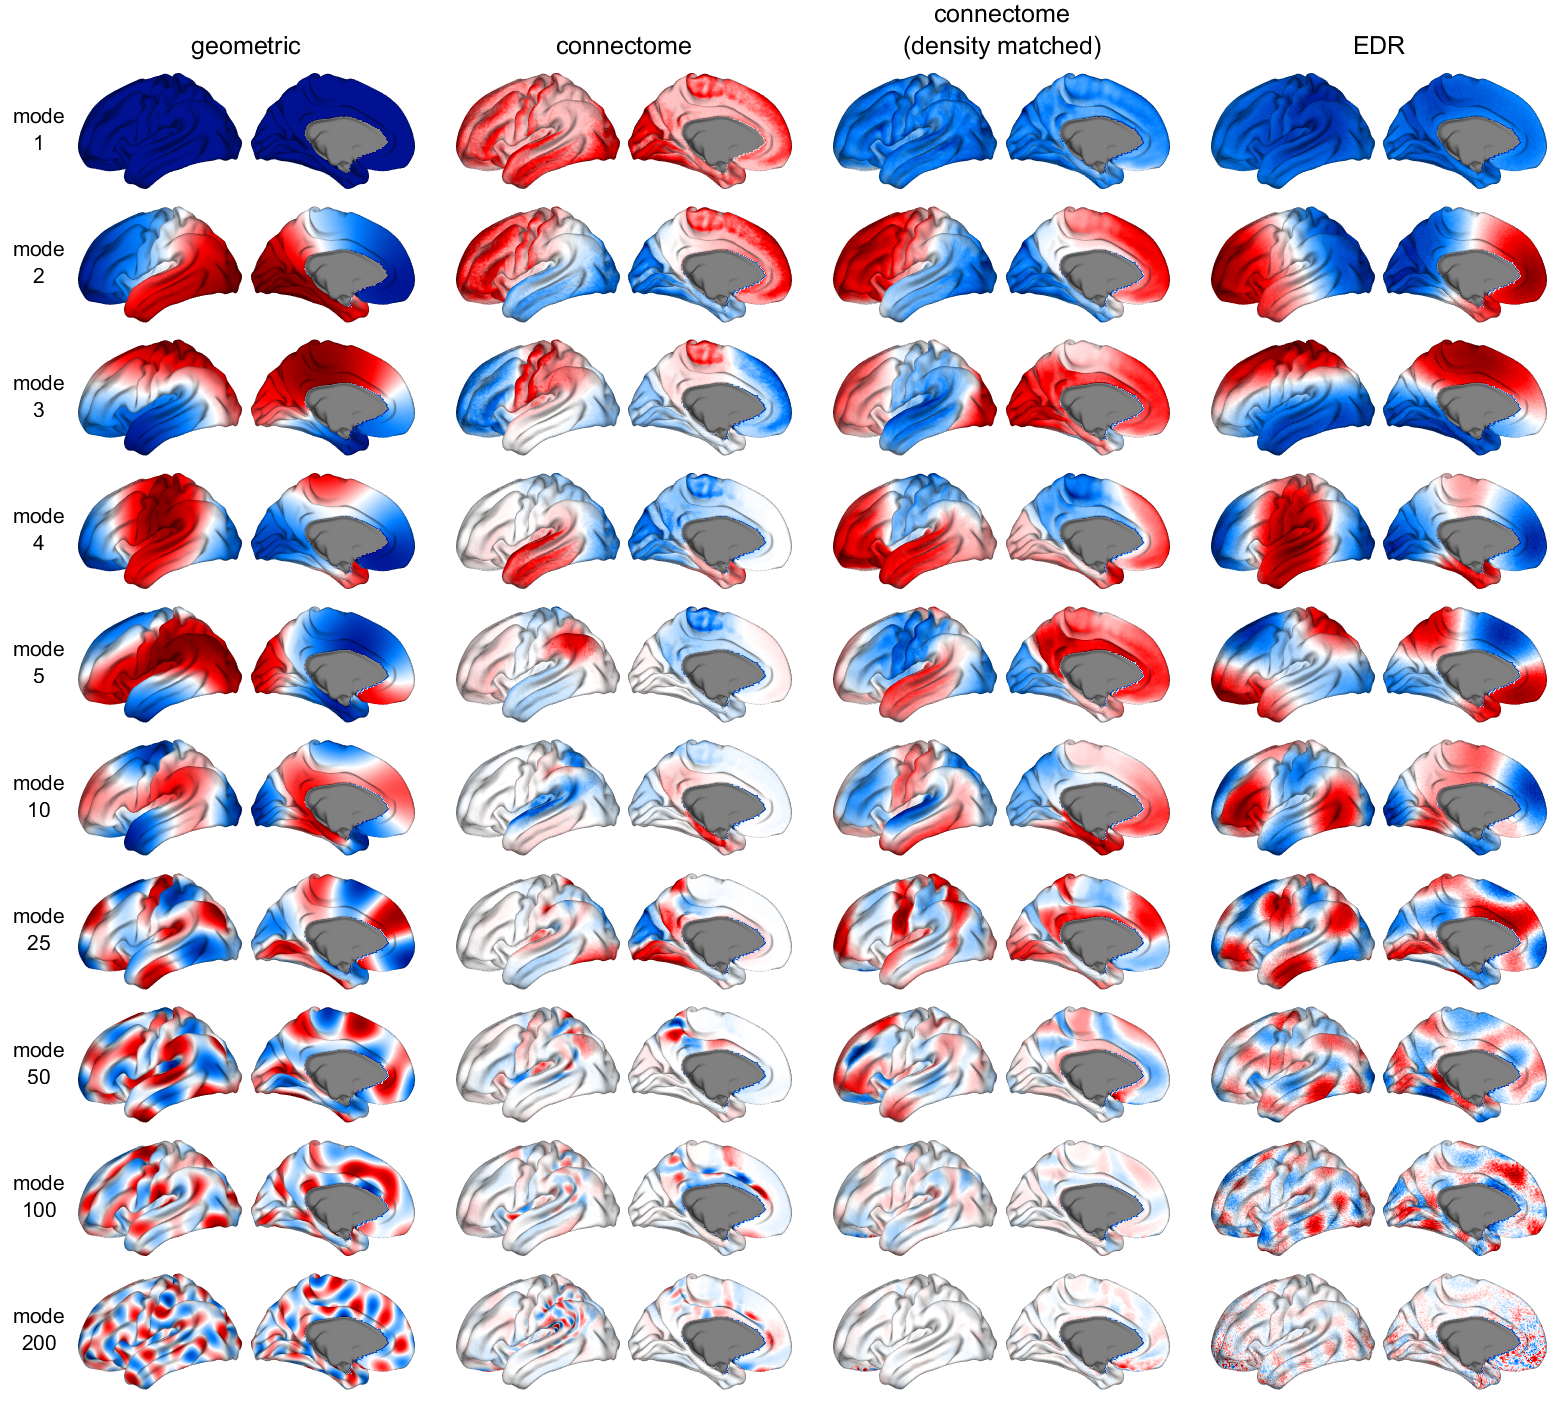
\includegraphics[width=0.9\textwidth]{fig/extended_fig_1.pdf}
	\caption{
	} \label{fig:extended_fig_1}
\end{figure}


\begin{figure}[!htb] 
	\centering
	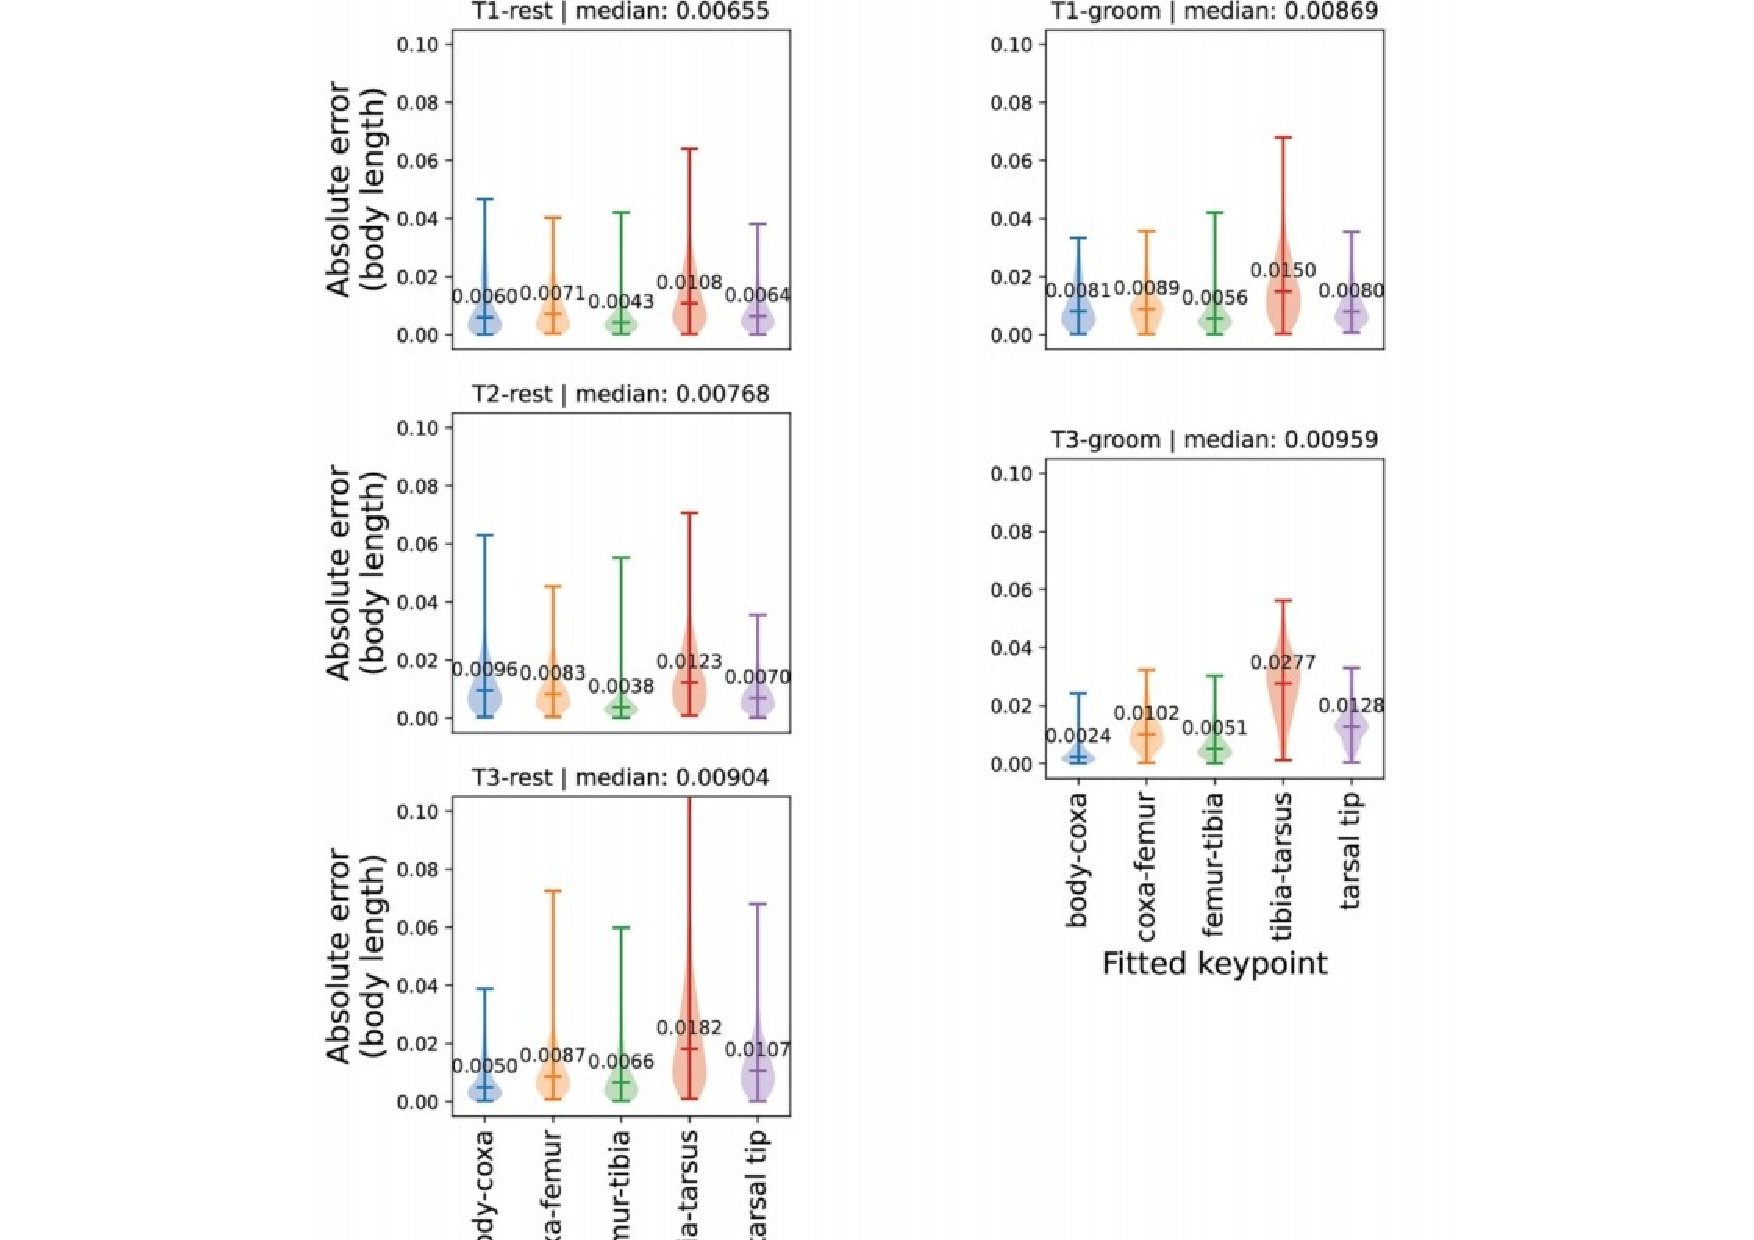
\includegraphics[width=0.9\textwidth]{fig/extended_fig_2.pdf}
	\caption{
	} \label{fig:extended_fig_2}
\end{figure}


\begin{figure}[!htb] 
	\centering
	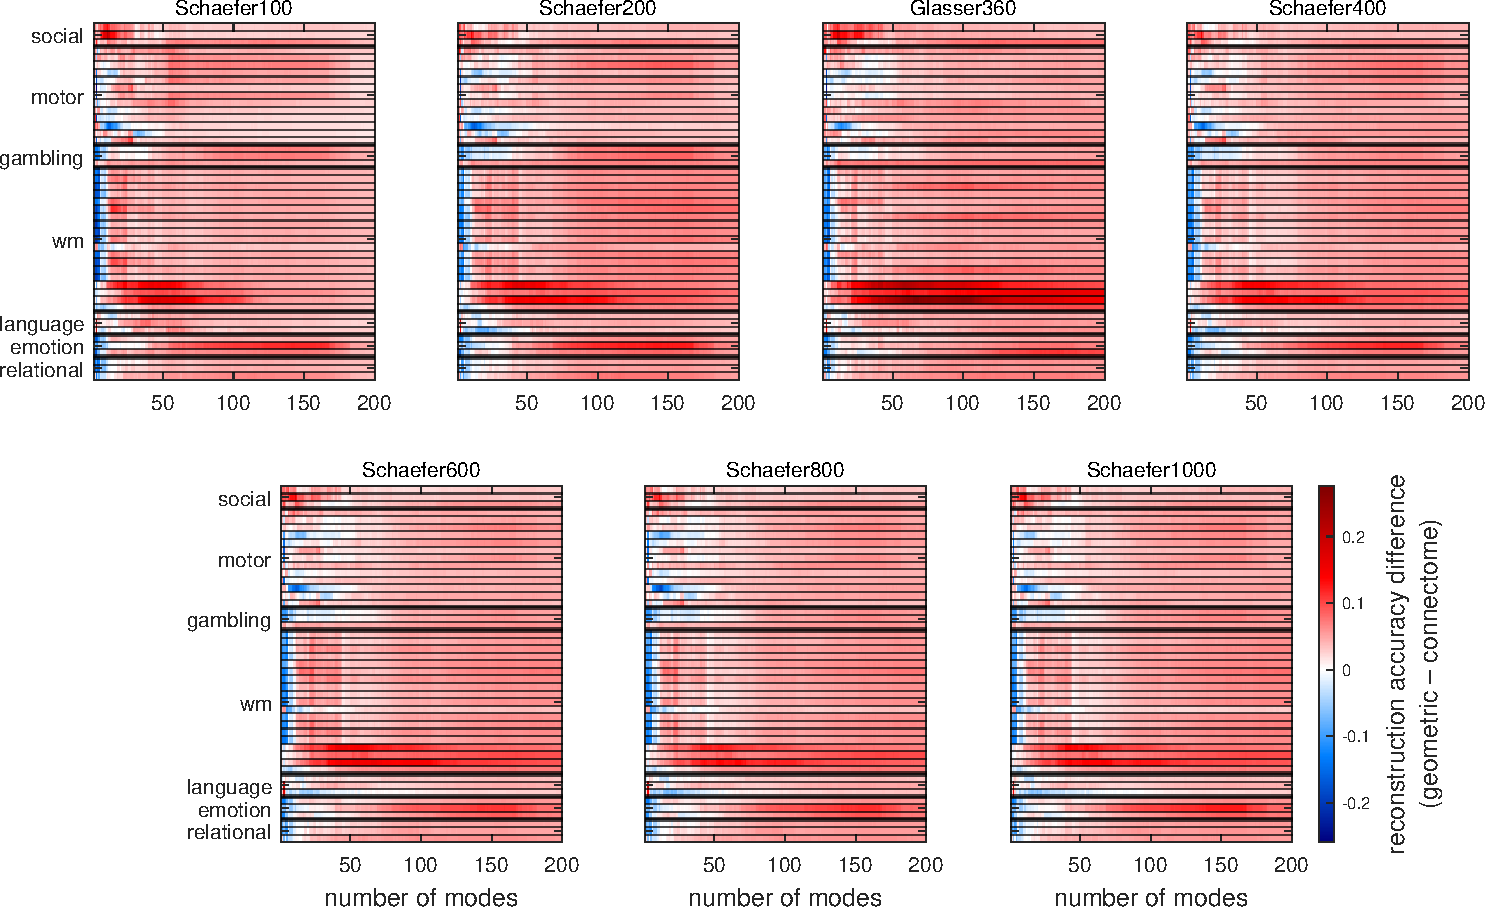
\includegraphics[width=0.9\textwidth]{fig/extended_fig_3.pdf}
	\caption{}
	\label{fig:extended_fig_3}
\end{figure}


\begin{figure}[!htb] 
	\centering
	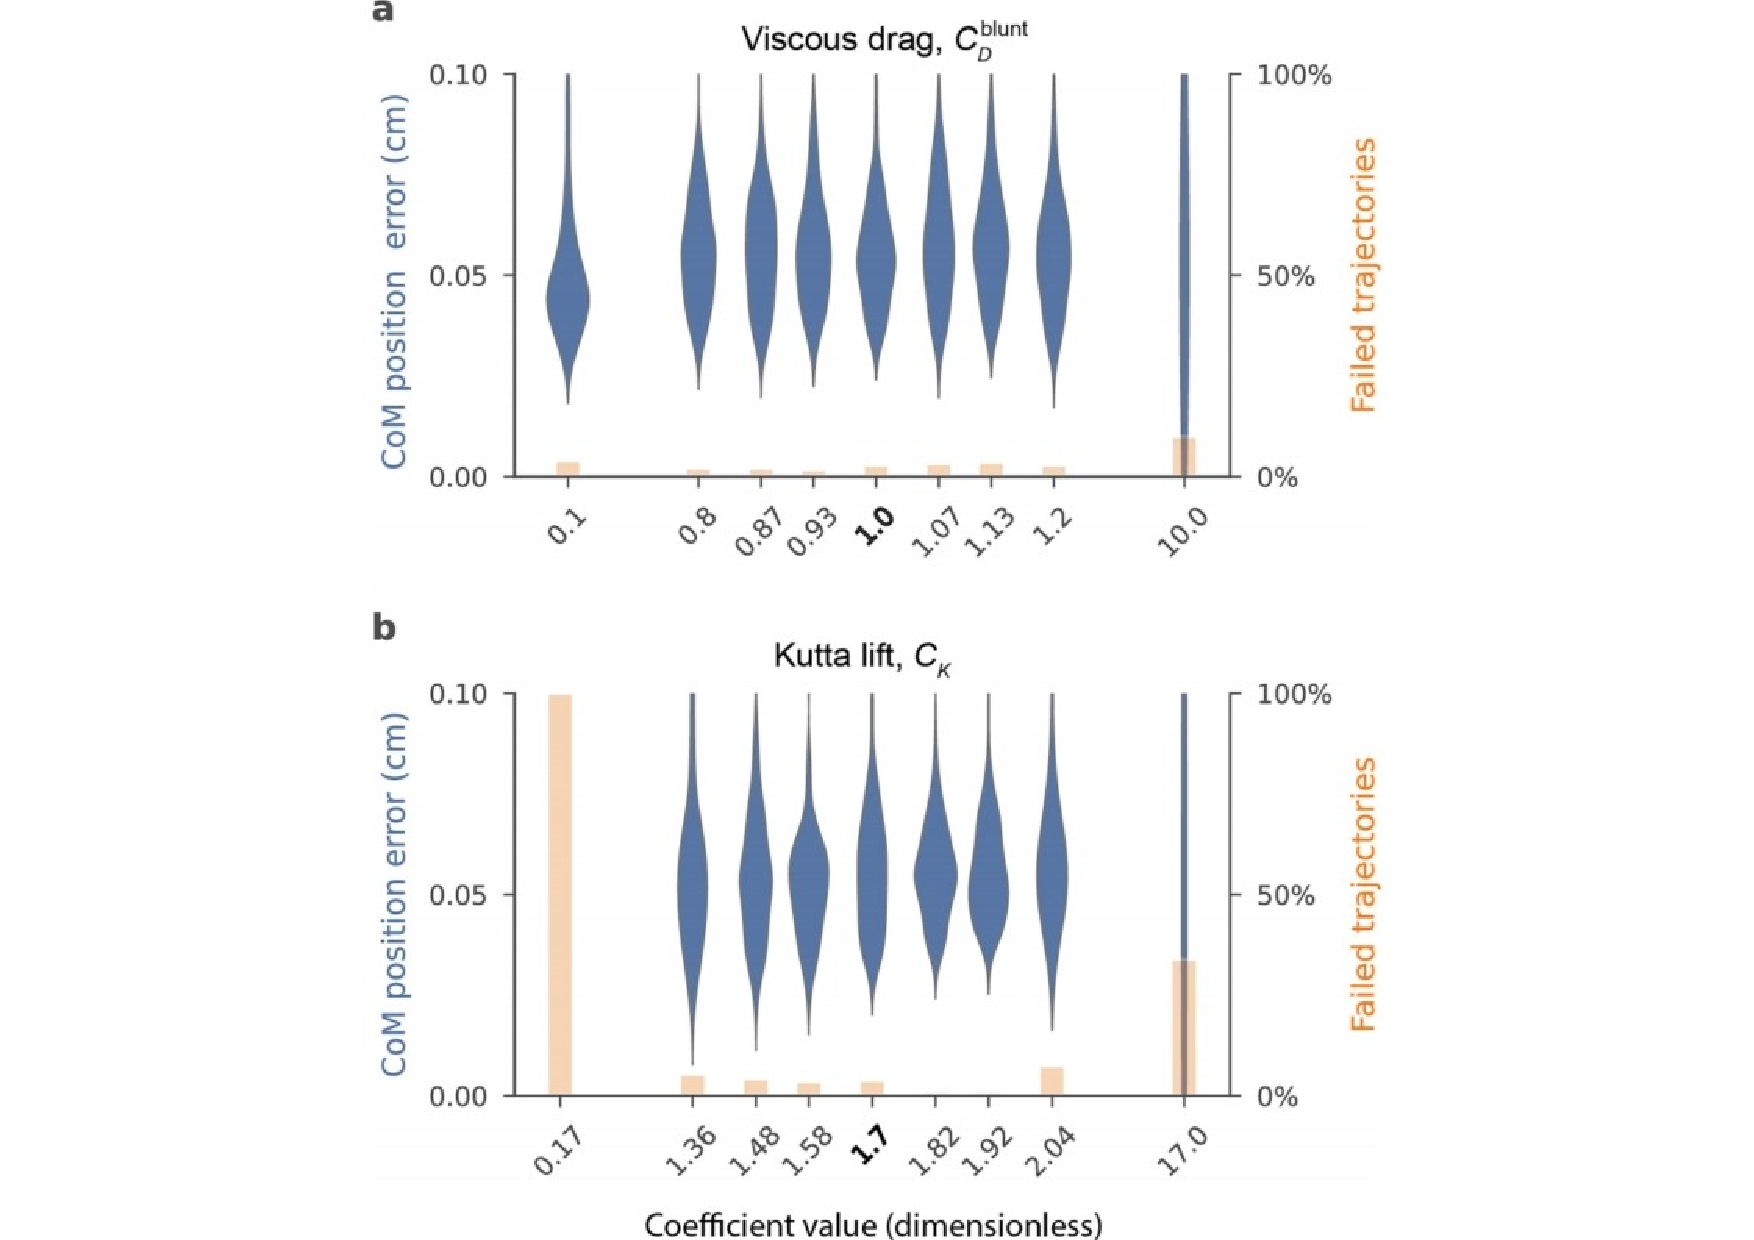
\includegraphics[width=0.9\textwidth]{fig/extended_fig_4.pdf}
	\caption{}
	\label{fig:extended_fig_4}
\end{figure}


\begin{figure}[!htb] 
	\centering
	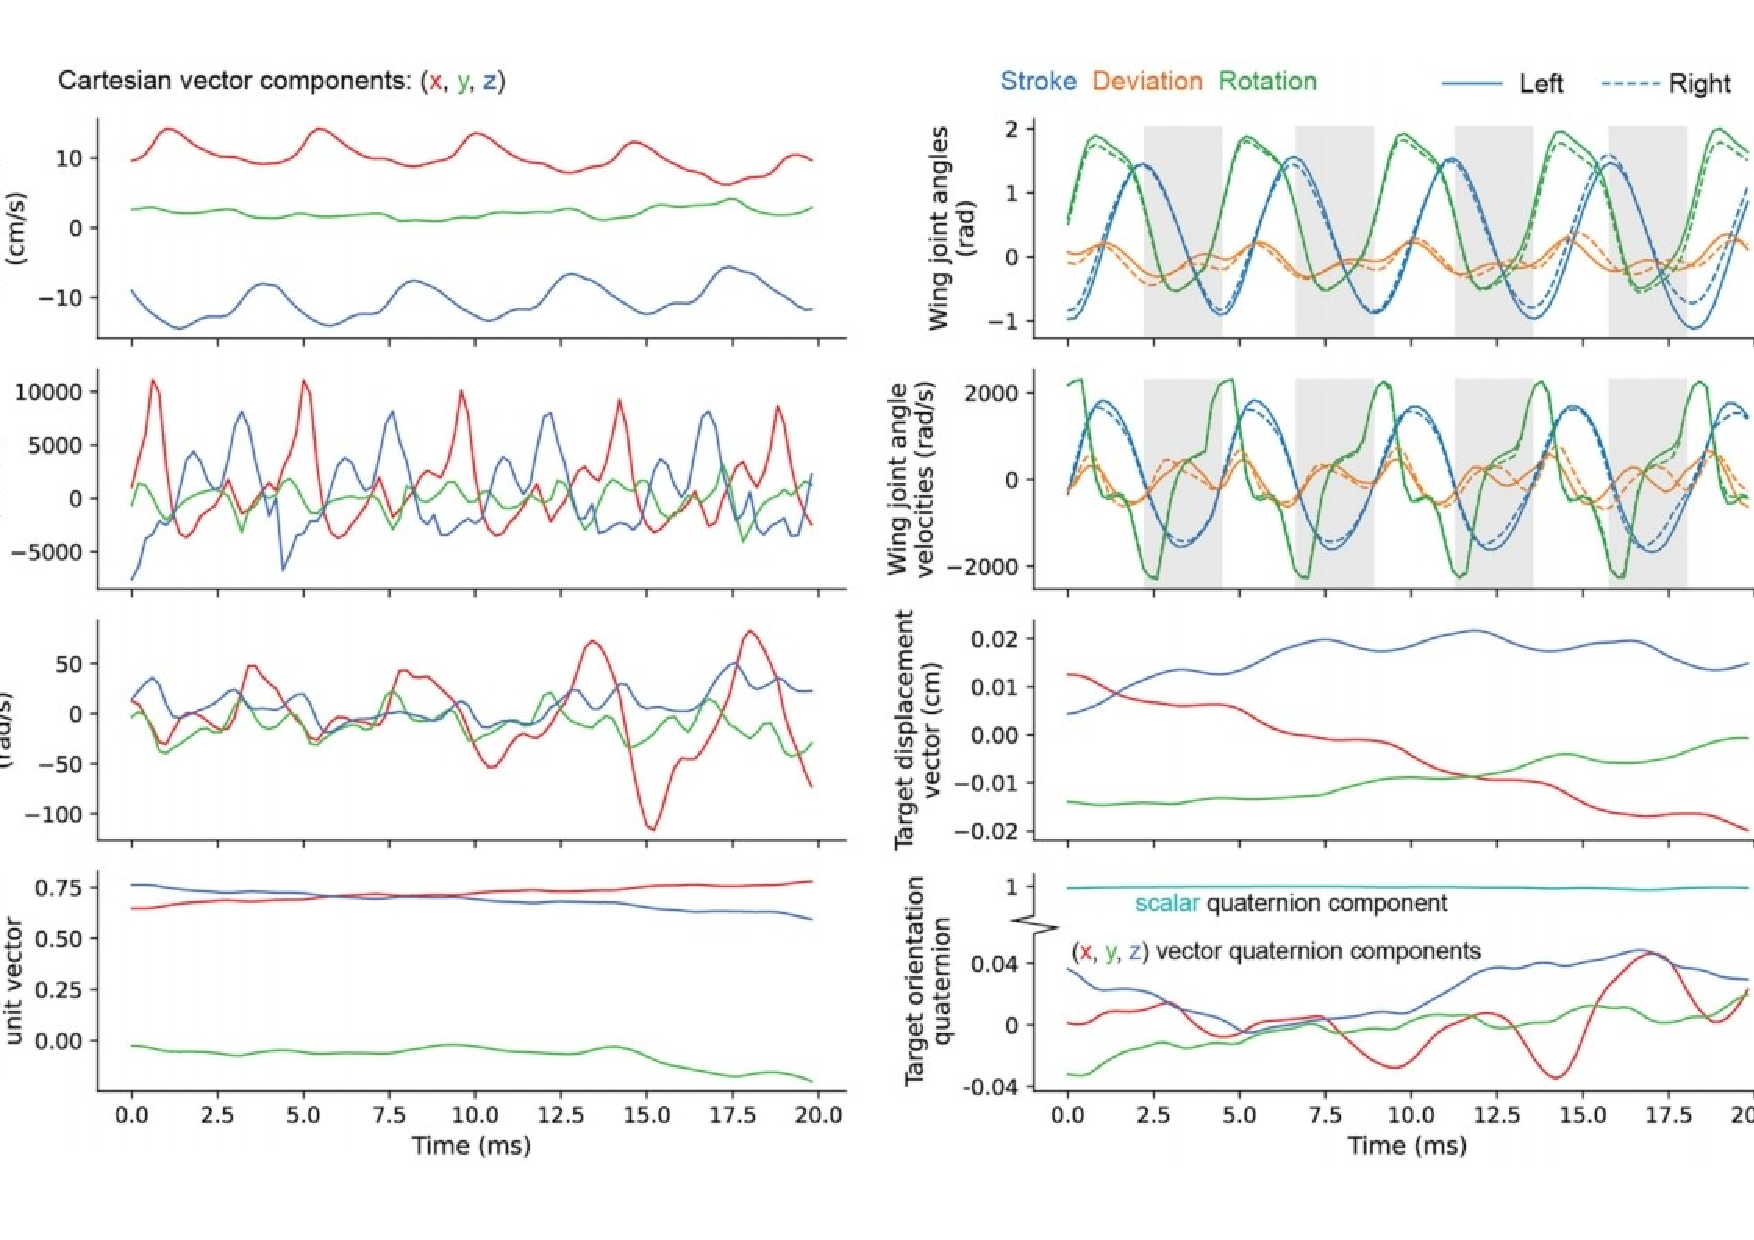
\includegraphics[width=0.9\textwidth]{fig/extended_fig_5.pdf}
	\caption{}
	\label{fig:extended_fig_5}
\end{figure}



\begin{figure}[!htb] 
	\centering
	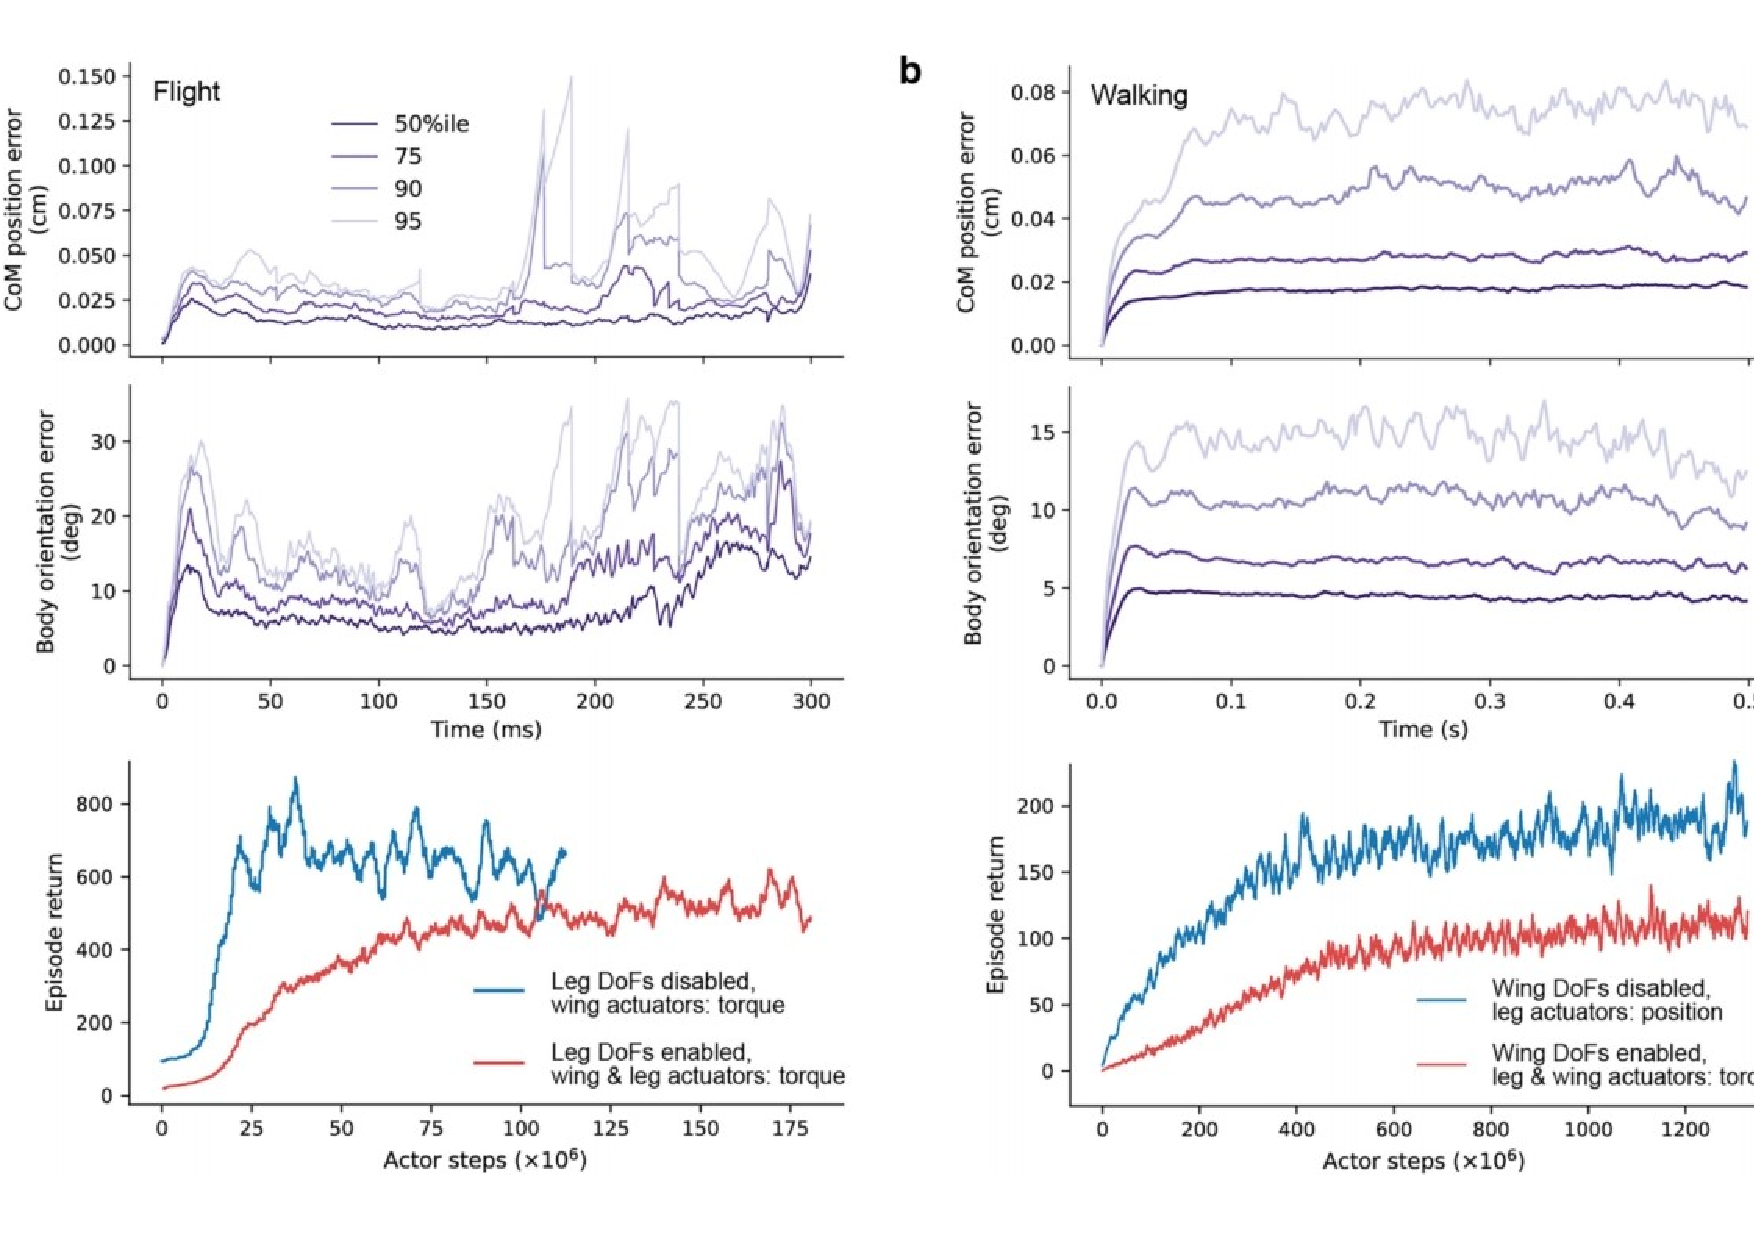
\includegraphics[width=0.9\textwidth]{fig/extended_fig_6.pdf}
	\caption{}
	\label{fig:extended_fig_6}
\end{figure}


\begin{figure}[!htb] 
	\centering
	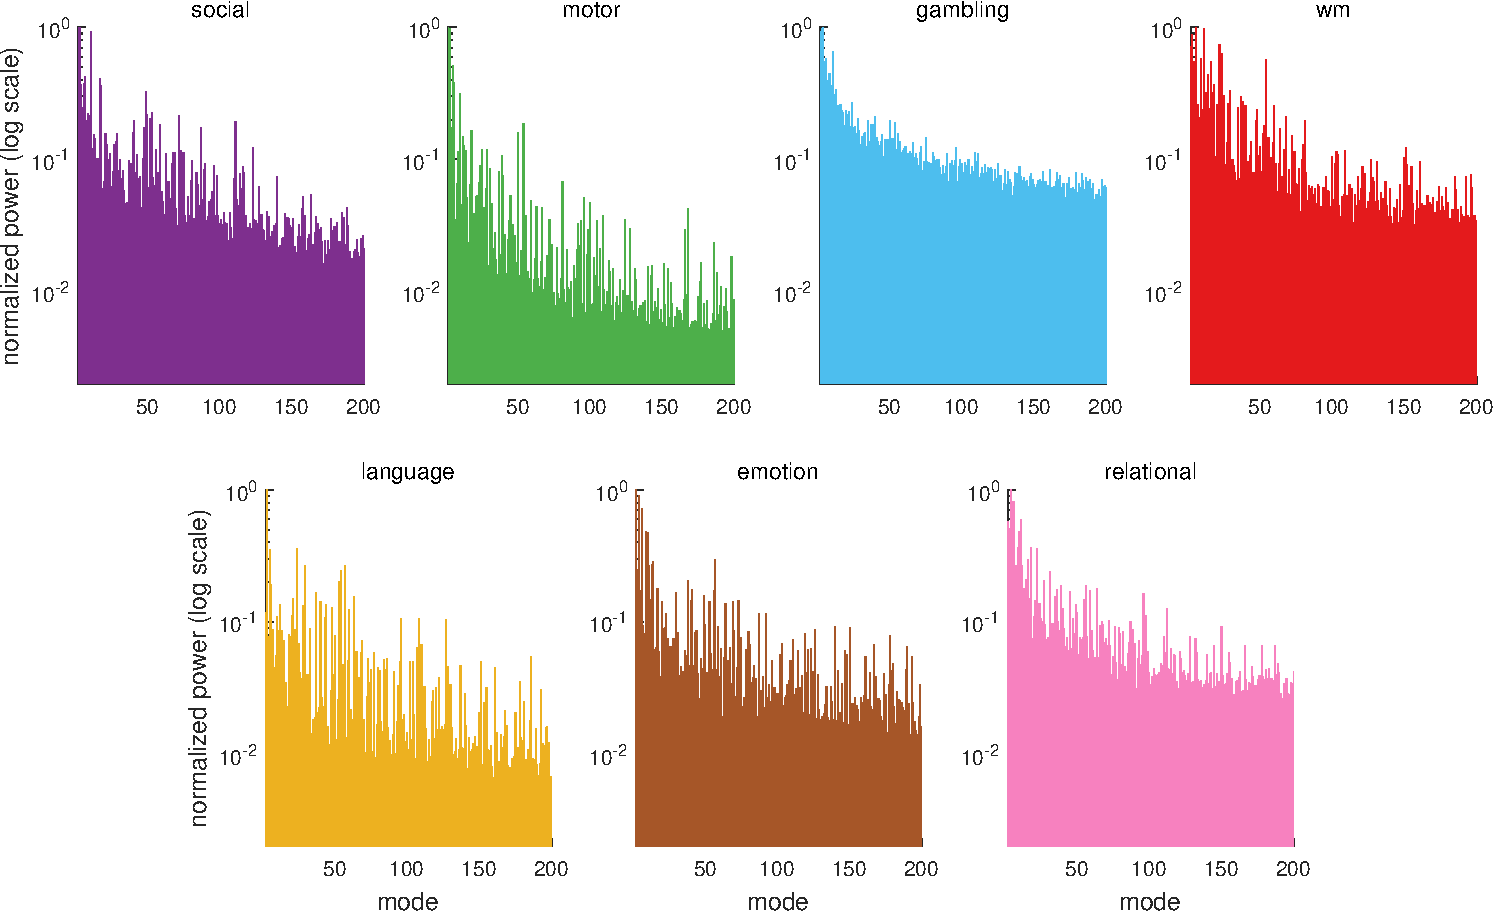
\includegraphics[width=0.9\textwidth]{fig/extended_fig_7.pdf}
	\caption{}
	\label{fig:extended_fig_7}
\end{figure}


\begin{figure}[!htb] 
	\centering
	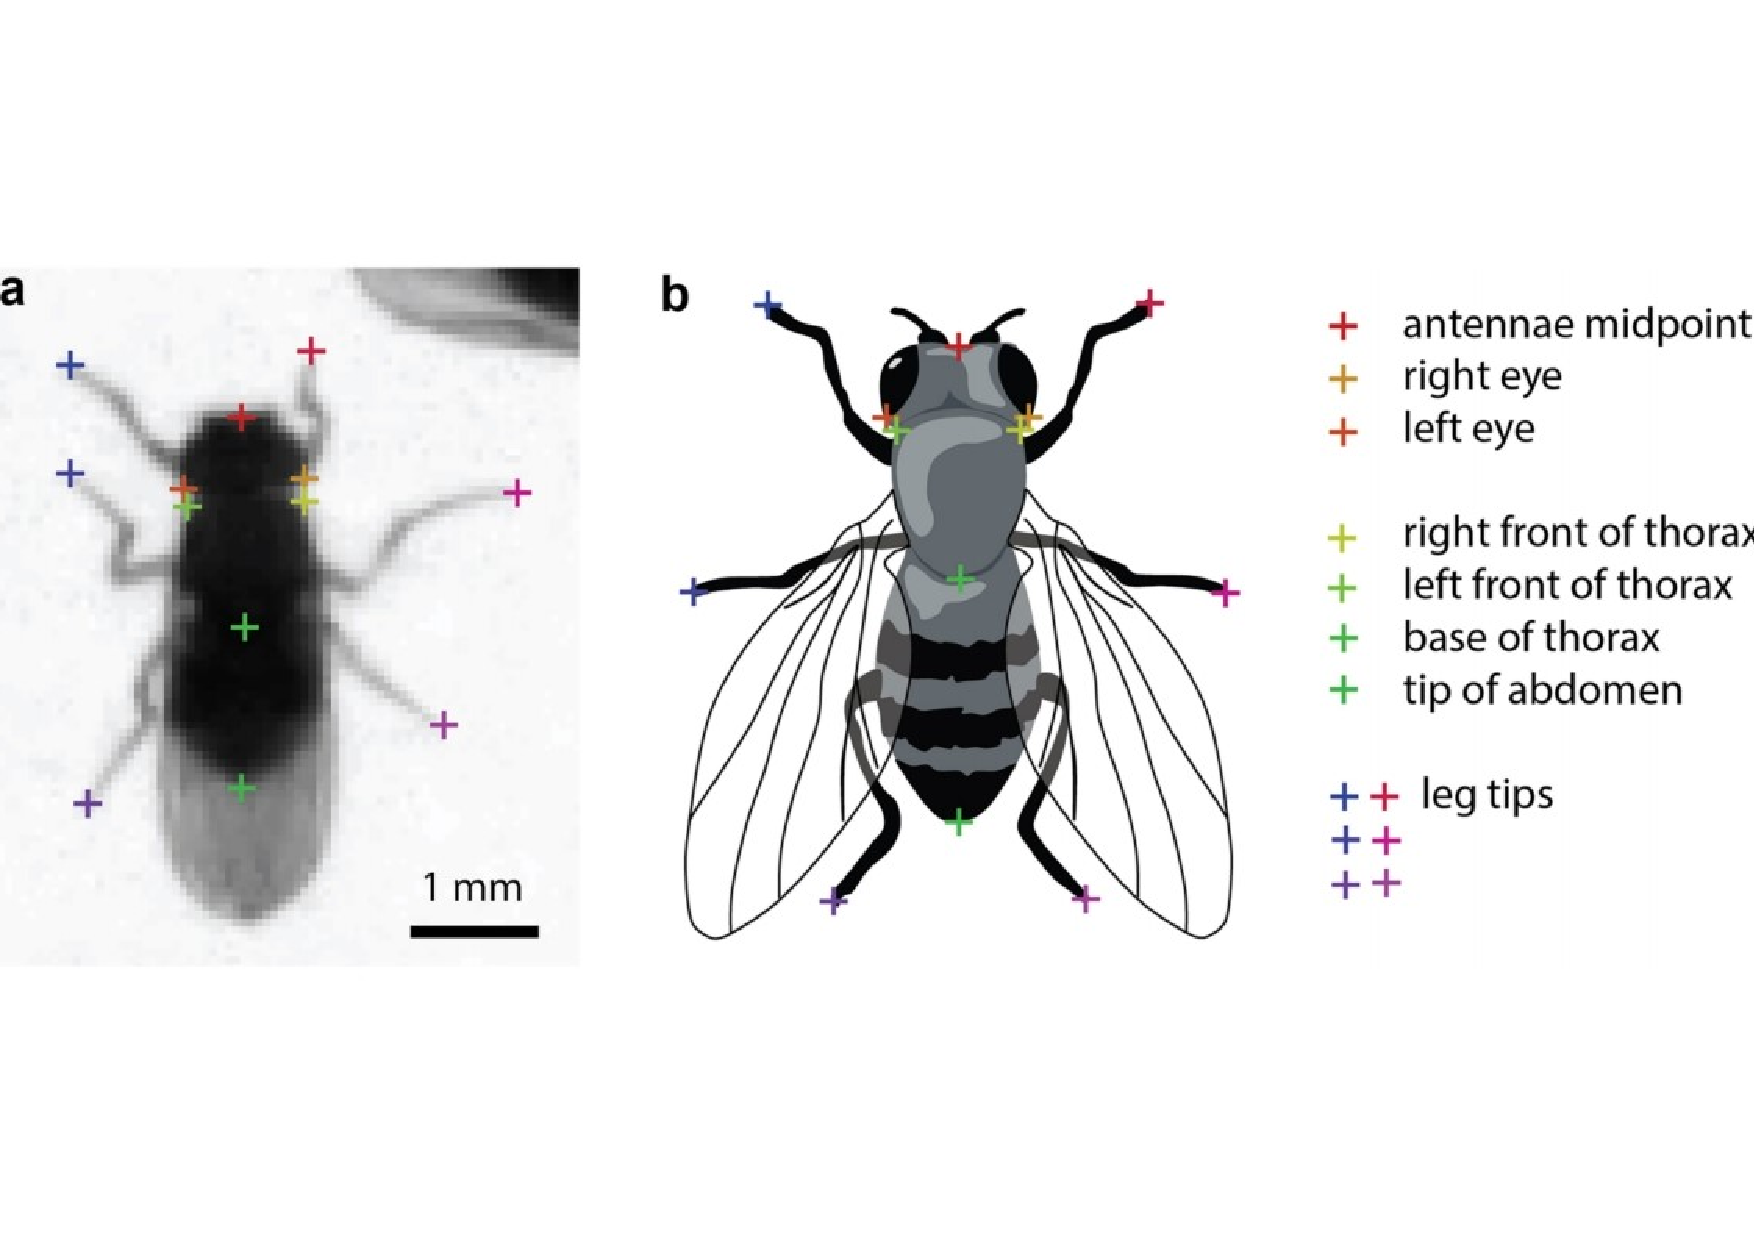
\includegraphics[width=0.9\textwidth]{fig/extended_fig_8.pdf}
	\caption{}
	\label{fig:extended_fig_8}
\end{figure}


\begin{figure}[!htb] 
	\centering
	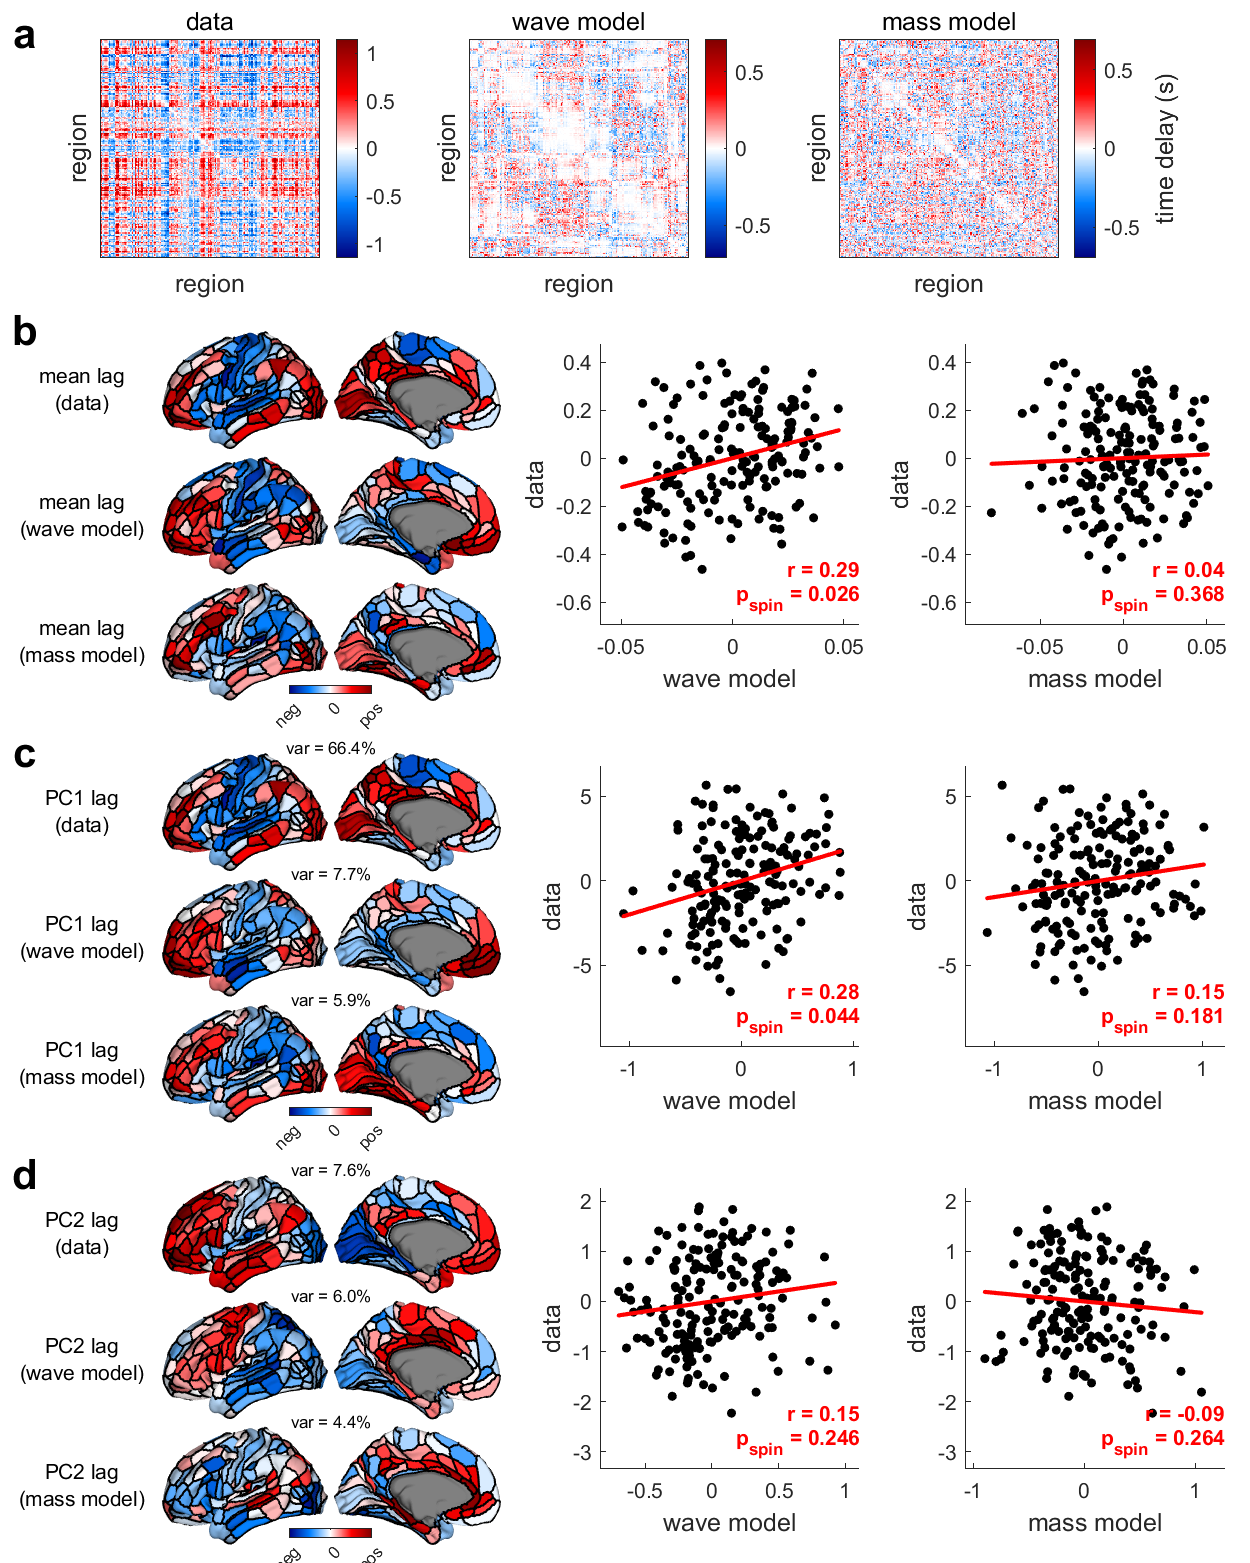
\includegraphics[width=0.9\textwidth]{fig/extended_fig_9.pdf}
	\caption{}
	\label{fig:extended_fig_9}
\end{figure}


\begin{figure}[!htb] 
	\centering
	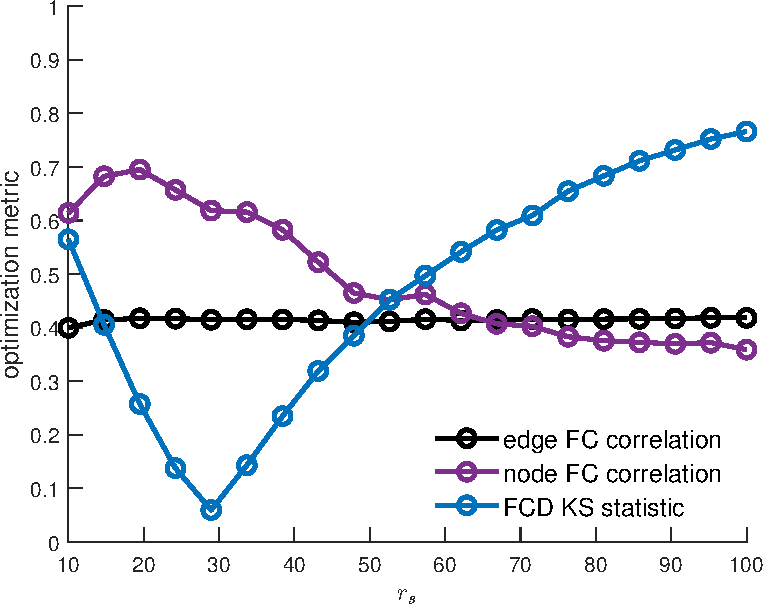
\includegraphics[width=0.9\textwidth]{fig/extended_fig_10.pdf}
	\caption{}
	\label{fig:extended_fig_10}
\end{figure}



\section{Conclusion}\label{sec13}

Conclusions may be used to restate your hypothesis or research question, restate your major findings, explain the relevance and the added value of your work, highlight any limitations of your study, describe future directions for research and recommendations. 

In some disciplines use of Discussion or 'Conclusion' is interchangeable. It is not mandatory to use both. Please refer to Journal-level guidance for any specific requirements. 

\backmatter

\bmhead{Supplementary information}

If your article has accompanying supplementary file/s please state so here. 

Authors reporting data from electrophoretic gels and blots should supply the full unprocessed scans for key as part of their Supplementary information. This may be requested by the editorial team/s if it is missing.

Please refer to Journal-level guidance for any specific requirements.

\bmhead{Acknowledgements}

Acknowledgements are not compulsory. Where included they should be brief. Grant or contribution numbers may be acknowledged.

Please refer to Journal-level guidance for any specific requirements.

\section*{Declarations}

Some journals require declarations to be submitted in a standardised format. Please check the Instructions for Authors of the journal to which you are submitting to see if you need to complete this section. If yes, your manuscript must contain the following sections under the heading `Declarations':

\begin{itemize}
\item Funding
\item Conflict of interest/Competing interests (check journal-specific guidelines for which heading to use)
\item Ethics approval and consent to participate
\item Consent for publication
\item Data availability 
\item Materials availability
\item Code availability 
\item Author contribution
\end{itemize}

\noindent
If any of the sections are not relevant to your manuscript, please include the heading and write `Not applicable' for that section. 

%%===================================================%%
%% For presentation purpose, we have included        %%
%% \bigskip command. Please ignore this.             %%
%%===================================================%%
\bigskip
\begin{flushleft}%
Editorial Policies for:

\bigskip\noindent
Springer journals and proceedings: \url{https://www.springer.com/gp/editorial-policies}

\bigskip\noindent
Nature Portfolio journals: \url{https://www.nature.com/nature-research/editorial-policies}

\bigskip\noindent
\textit{Scientific Reports}: \url{https://www.nature.com/srep/journal-policies/editorial-policies}

\bigskip\noindent
BMC journals: \url{https://www.biomedcentral.com/getpublished/editorial-policies}
\end{flushleft}

\begin{appendices}
	
	
\section{Supplementary information} \label{secInfo}

\subsection{Neural field theory} \label{sec:NFT} 

\subsection{Human Connectome Project data} \label{sec:sup_2}

\subsubsection{Task-evoked data} \label{sec:sup_2_1}

\subsubsection{Task-free resting-state data} \label{sec:sup_2_2}

\subsubsection{Connectome data} \label{sec:sup_2_3}


\subsection{Individual-specific cortical eigenmodes} \label{sec:individual_specific}

\subsection{Effect of connectome thresholding on connectome eigenmodes} \label{sec:thresholding_effect}

\subsection{Comparison between geometric eigenmodes and a functionally derived basis set} \label{sec:comparison_eigenmodes_derived}

\subsection{Comparison between geometric eigenmodes and Fourier basis sets} \label{sec:comparison_fourier}

\subsection{Modal power spectra of surrogate maps} \label{sec:modal_power_spectra}

\subsection{NFT wave model} \label{sec:NFT_wave}

\subsection{Optimization of the BEI neural mass model} \label{sec:mass_optimization}

\subsection{Lag threads algorithm} \label{sec:lag_threads}


\subsection{Supplementary table}\label{secA1}

\begin{table}[htbp]
	\centering
	\small
	\caption{eigenmodel}
	\begin{tabular}{ccc}
		\toprule
		feature         &        wavelength(nm)  & eigenmodel     \\
		\midrule
		0      &   -      &      1  \\
		1      &   297.7      &      2-4  \\
		2      &   171.9      &      5-9  \\
		3      &   121.5      &      10-16  \\
		4      &   94.1      &      17-25  \\
		5      &   76.9      &      26-36  \\
		6      &   65.0      &      37-49  \\
		7      &   56.3      &      50-64  \\
		8      &   49.6      &      65-81  \\
		9      &   44.4      &      82-100  \\
		10      &   40.1      &      101-121  \\
		11      &   35.5      &      122-144  \\
		12      &   33.7      &      145-169  \\
		13      &   31.2      &      170-196  \\
		14      &   29.1      &      197-225  \\
		
		\bottomrule
	\end{tabular}%
	\label{tab:spatial_wavelength}%
\end{table}%


\subsection{Supplementary figure}\label{secS1}



\begin{figure}[!htb] 
	\centering
	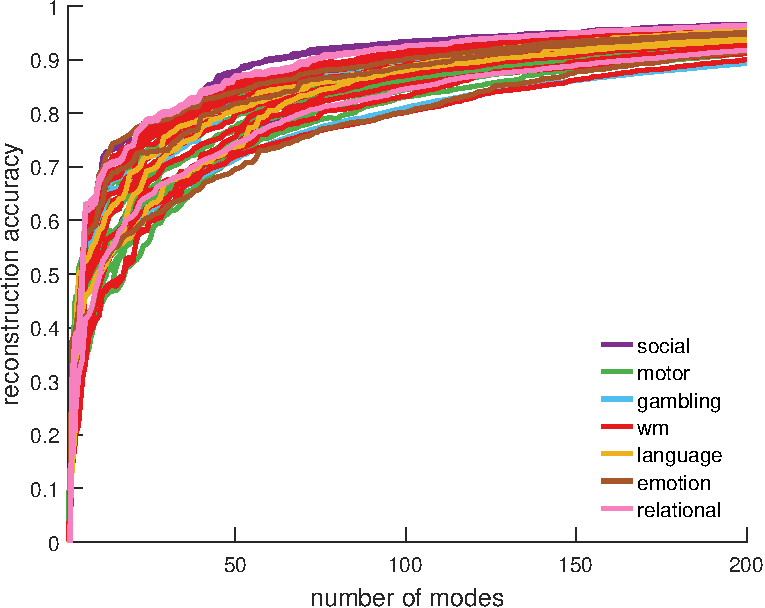
\includegraphics[width=0.7\textwidth]{fig/supp_1.pdf}
	\caption{} \label{fig:supp_1}
\end{figure}


\begin{figure}[!htb] 
	\centering
	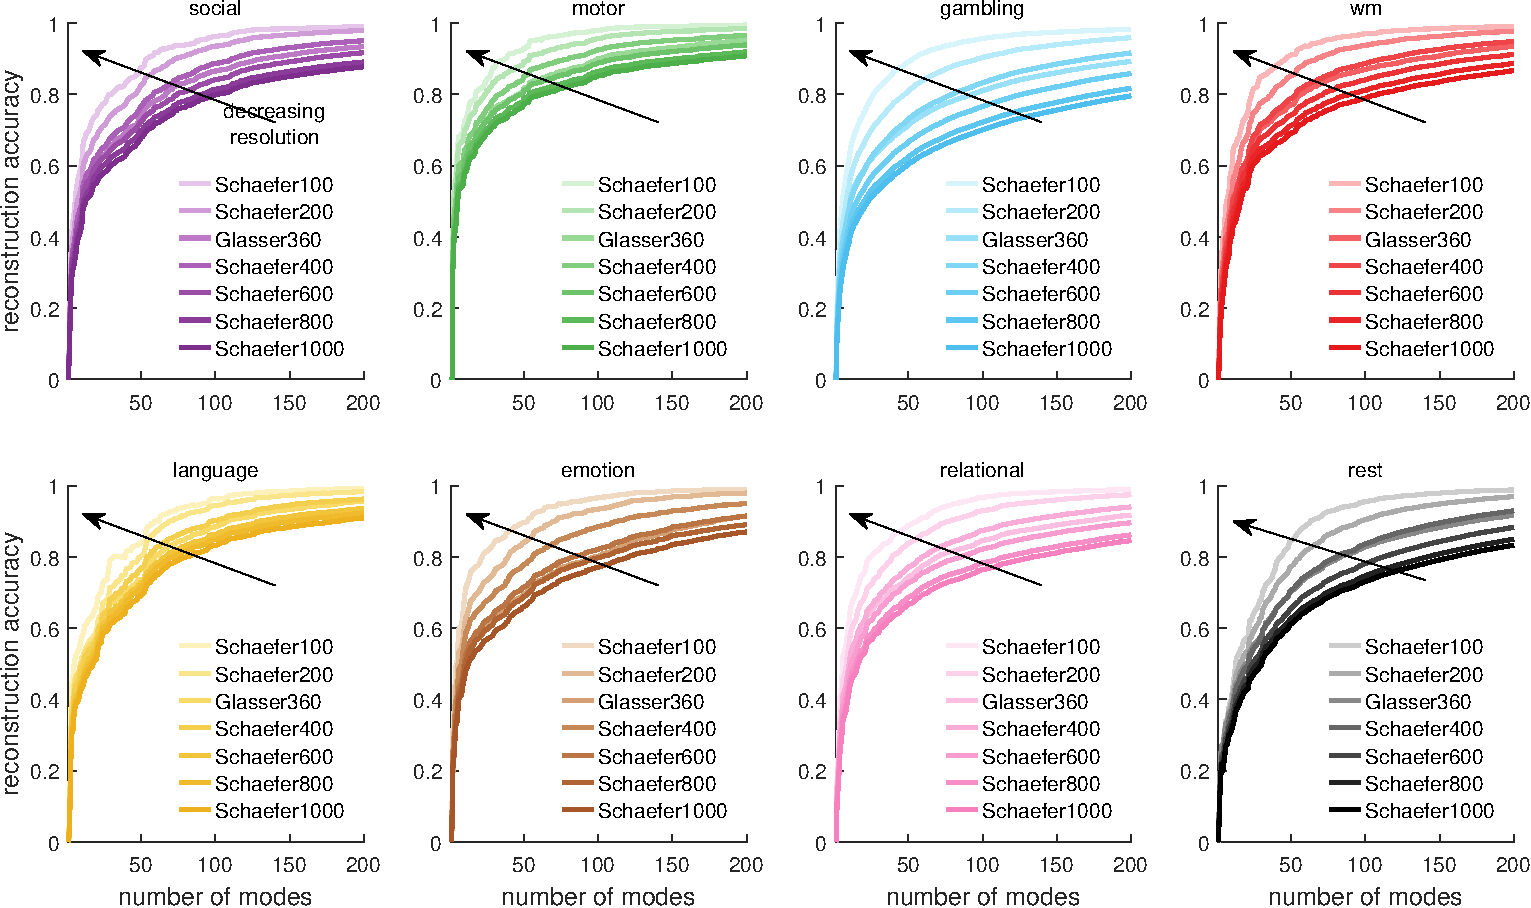
\includegraphics[width=0.85\textwidth]{fig/supp_2.pdf}
	\caption{} \label{fig:supp_2}
\end{figure}


\begin{figure}[!htb] 
	\centering
	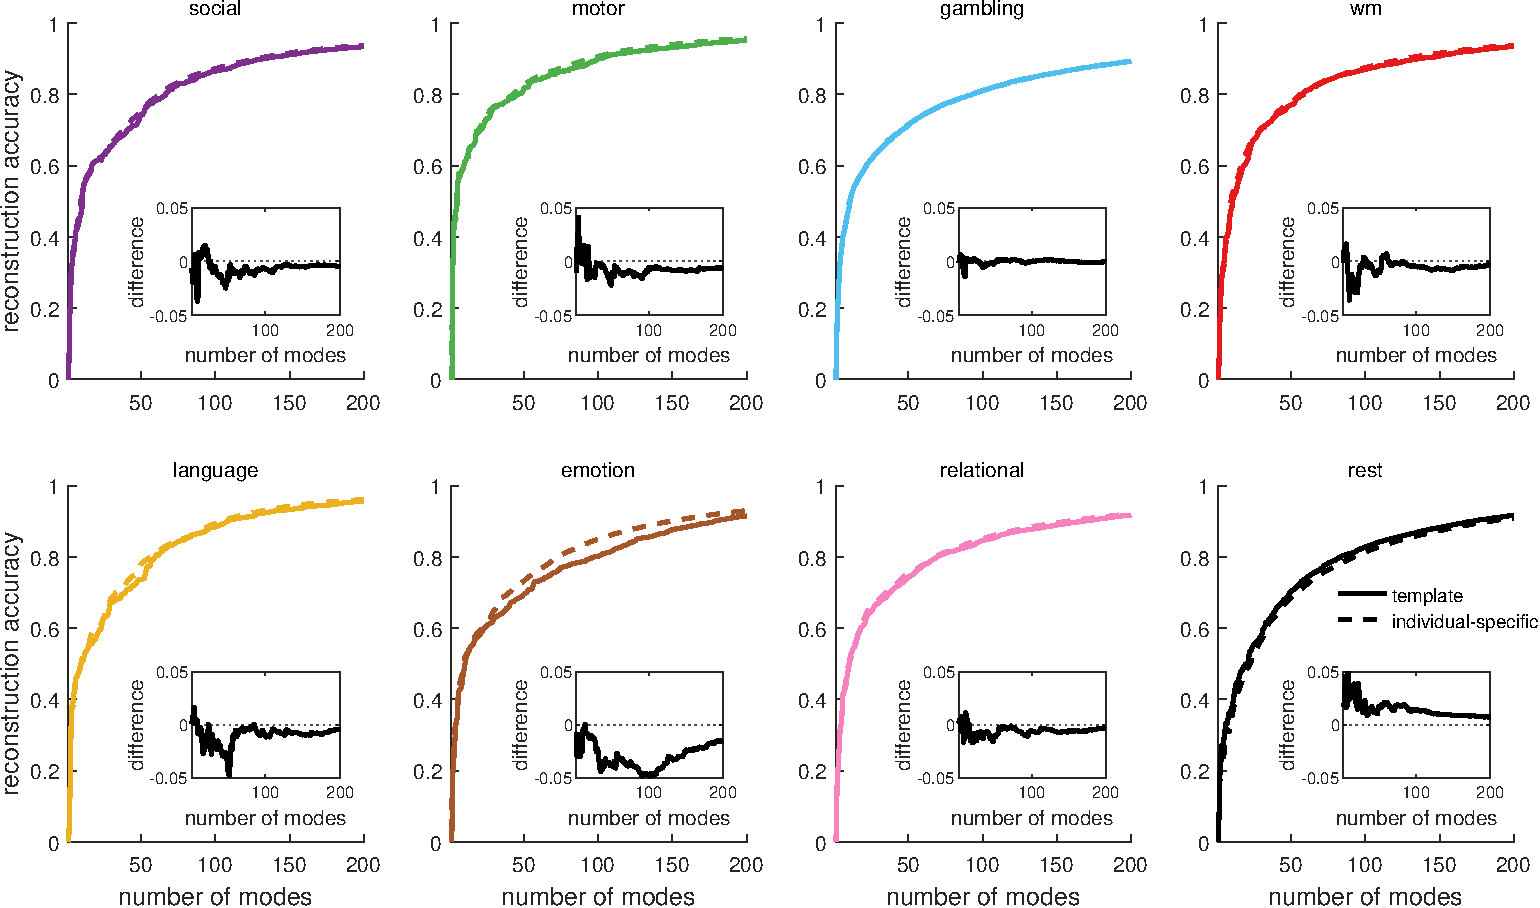
\includegraphics[width=0.85\textwidth]{fig/supp_3.pdf}
	\caption{} \label{fig:supp_3}
\end{figure}


\begin{figure}[!htb] 
	\centering
	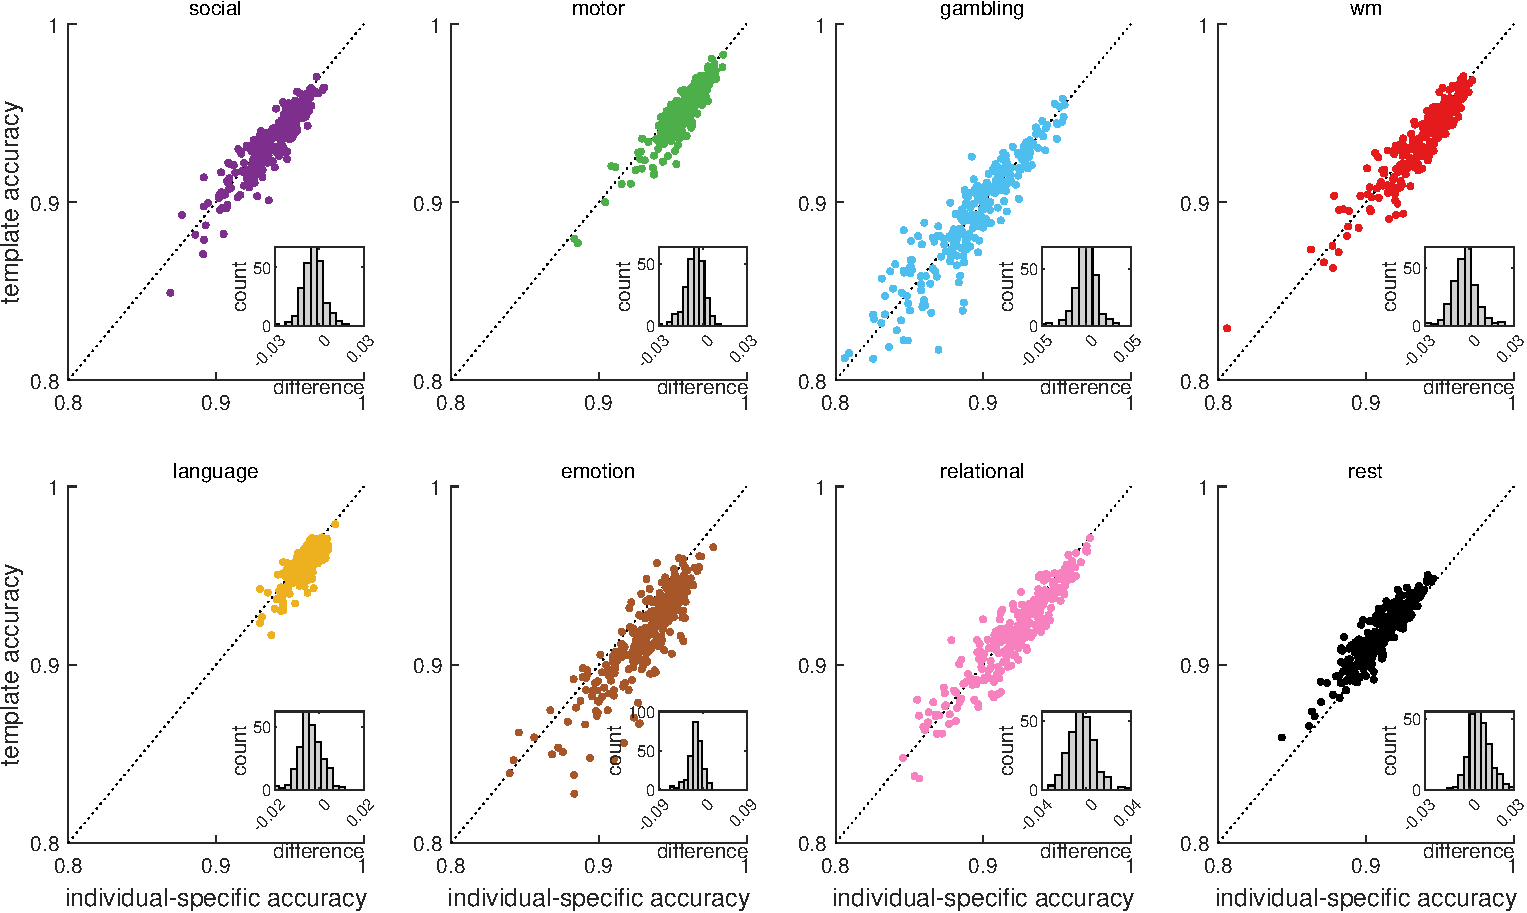
\includegraphics[width=0.85\textwidth]{fig/supp_4.pdf}
	\caption{} \label{fig:supp_4}
\end{figure}




\begin{figure}[!htb] 
	\centering
	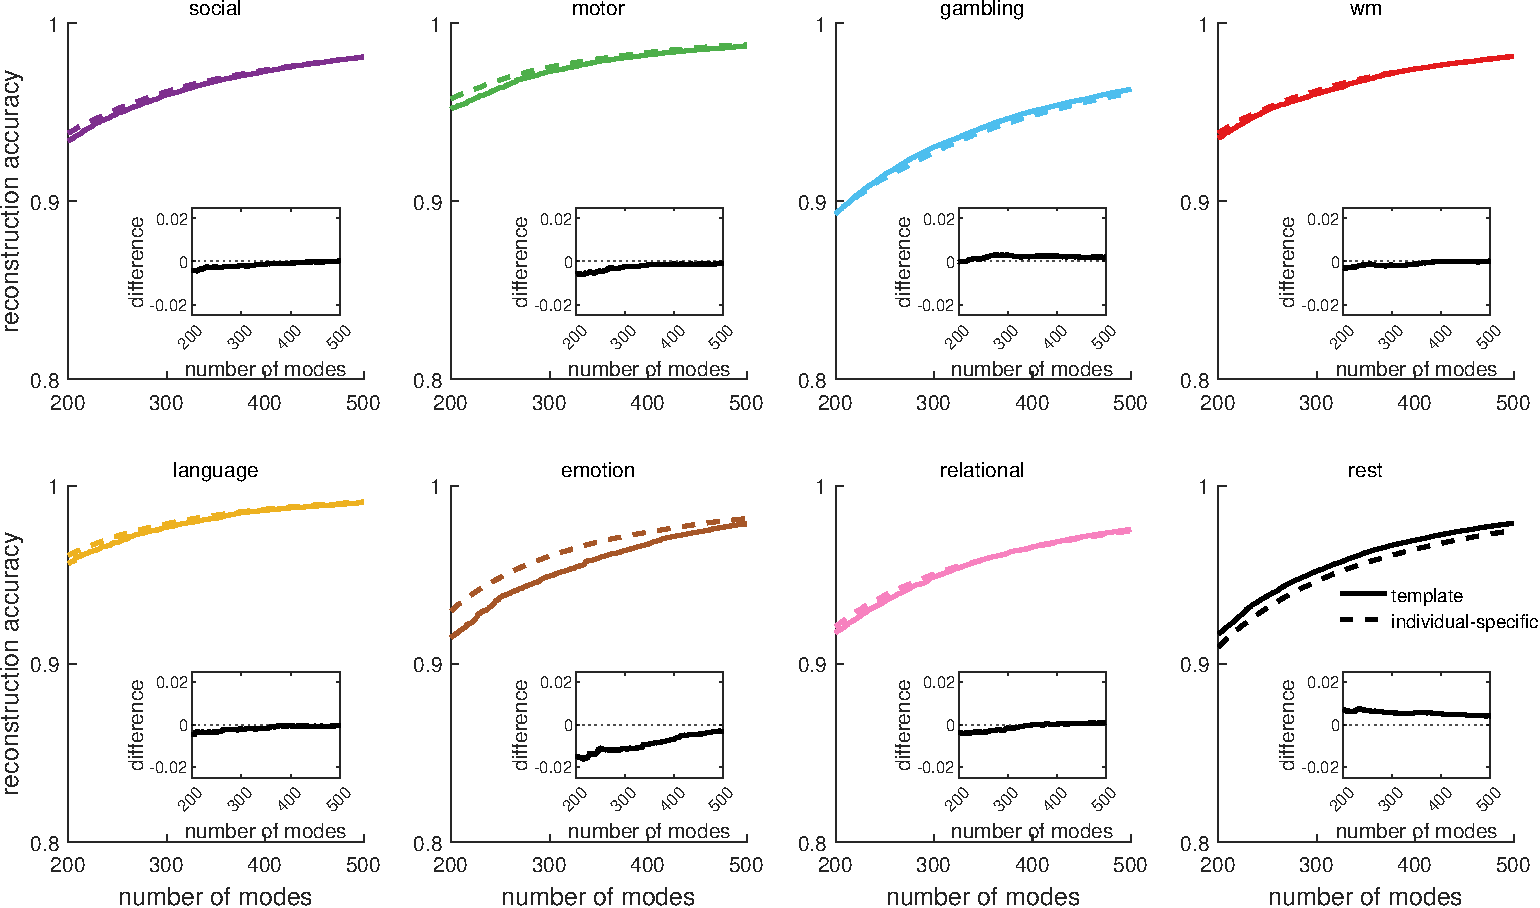
\includegraphics[width=0.85\textwidth]{fig/supp_5.pdf}
	\caption{} \label{fig:supp_5}
\end{figure}


\begin{figure}[!htb] 
	\centering
	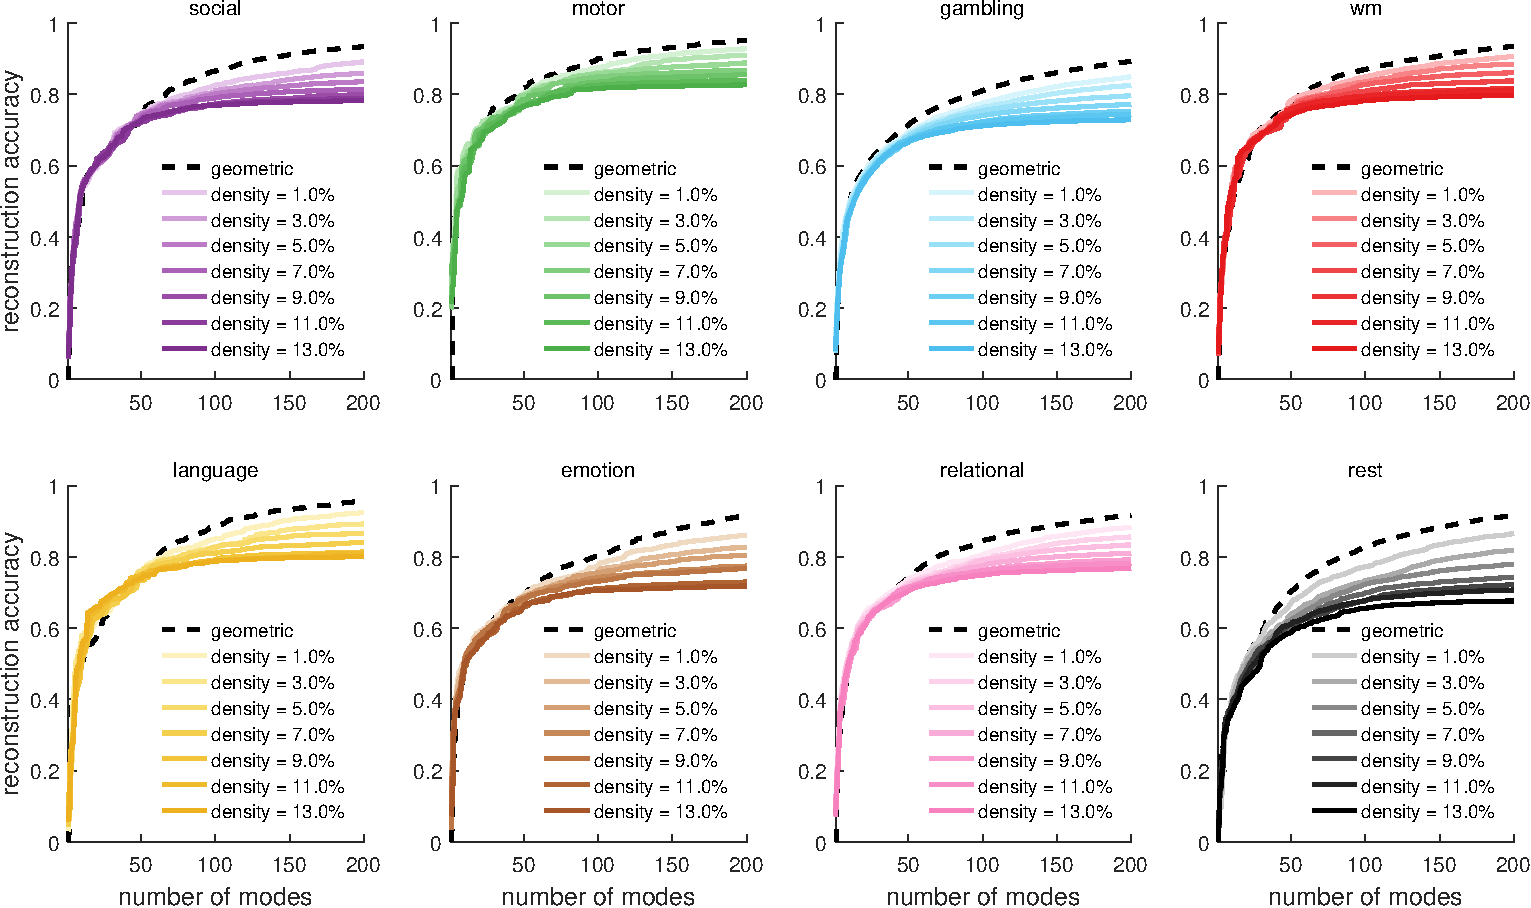
\includegraphics[width=0.85\textwidth]{fig/supp_6.pdf}
	\caption{
	} \label{fig:supp_6}
\end{figure}


\begin{figure}[!htb] 
	\centering
	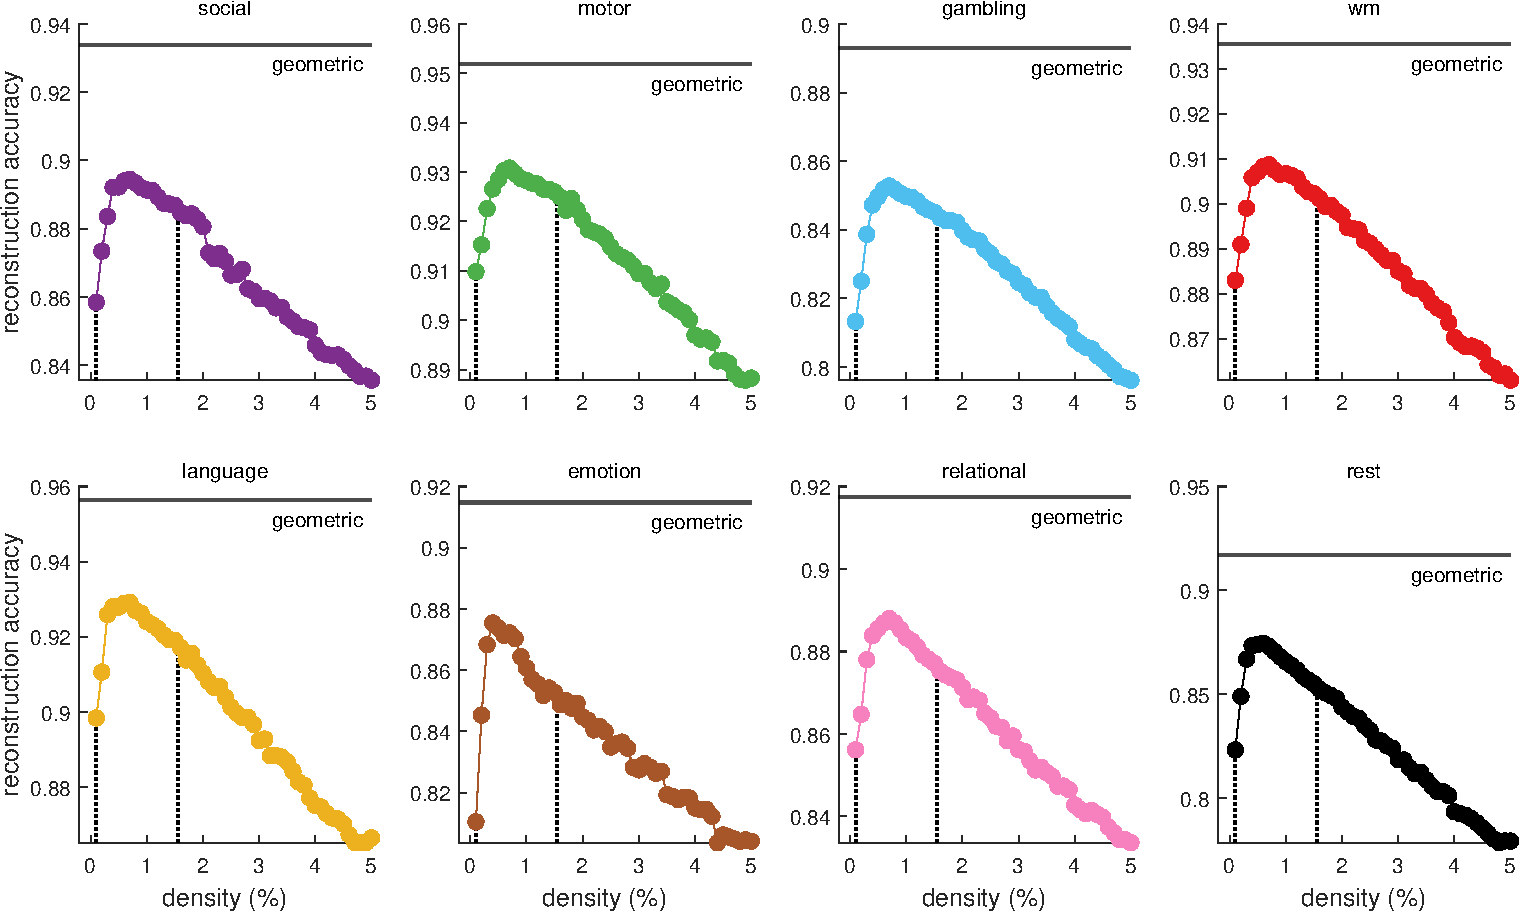
\includegraphics[width=1.0\textwidth]{fig/supp_7.pdf}
	\caption{
	} \label{fig:supp_7}
\end{figure}


\begin{figure}[!htb] 
	\centering
	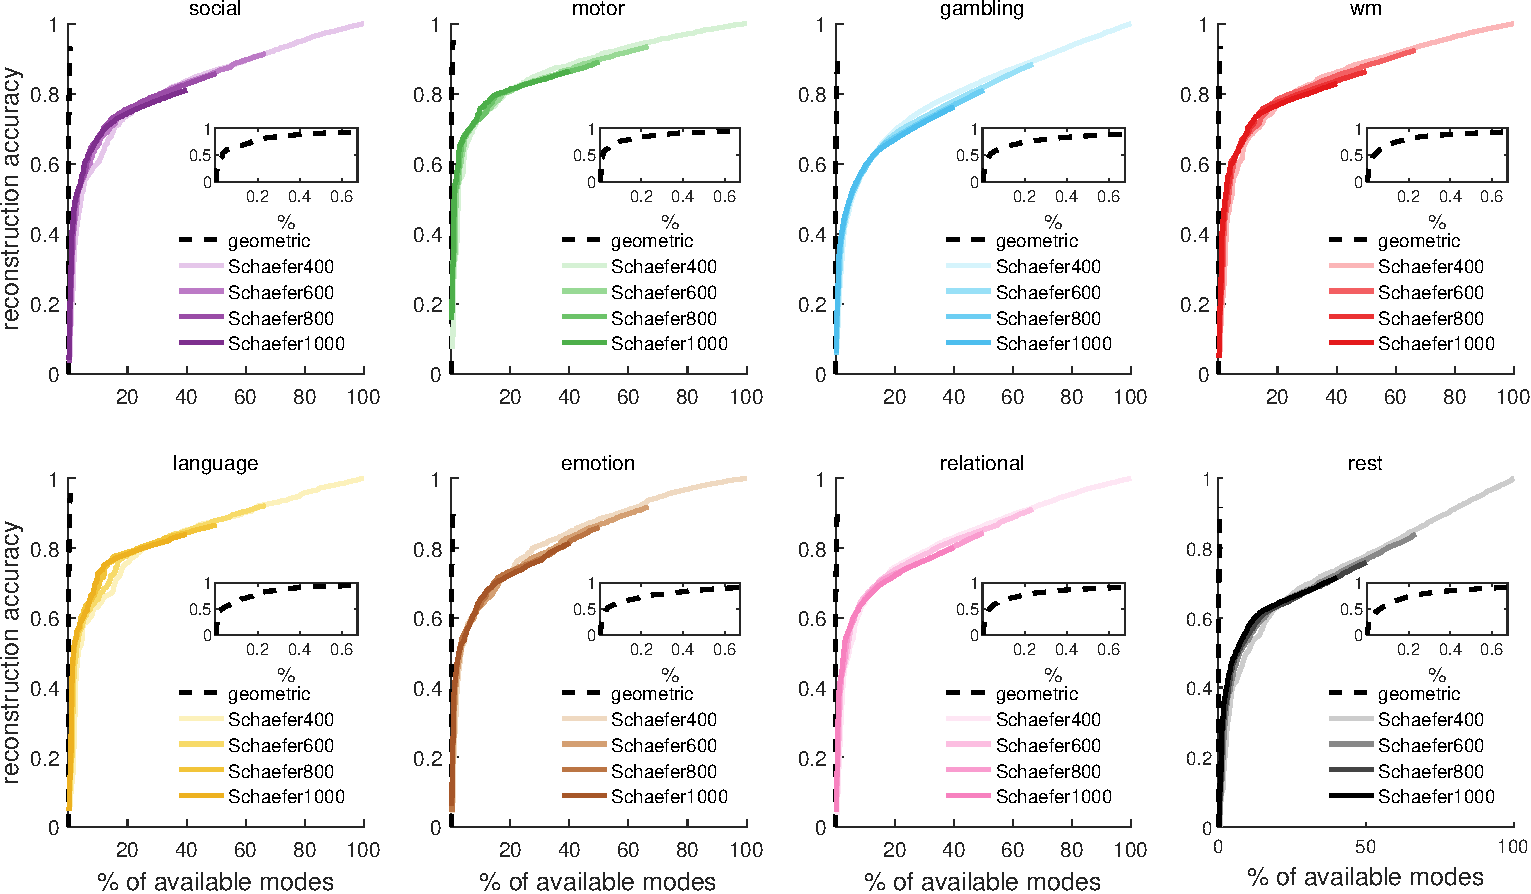
\includegraphics[width=0.85\textwidth]{fig/supp_8.pdf}
	\caption{
	} \label{fig:supp_8}
\end{figure}


\begin{figure}[!htb] 
	\centering
	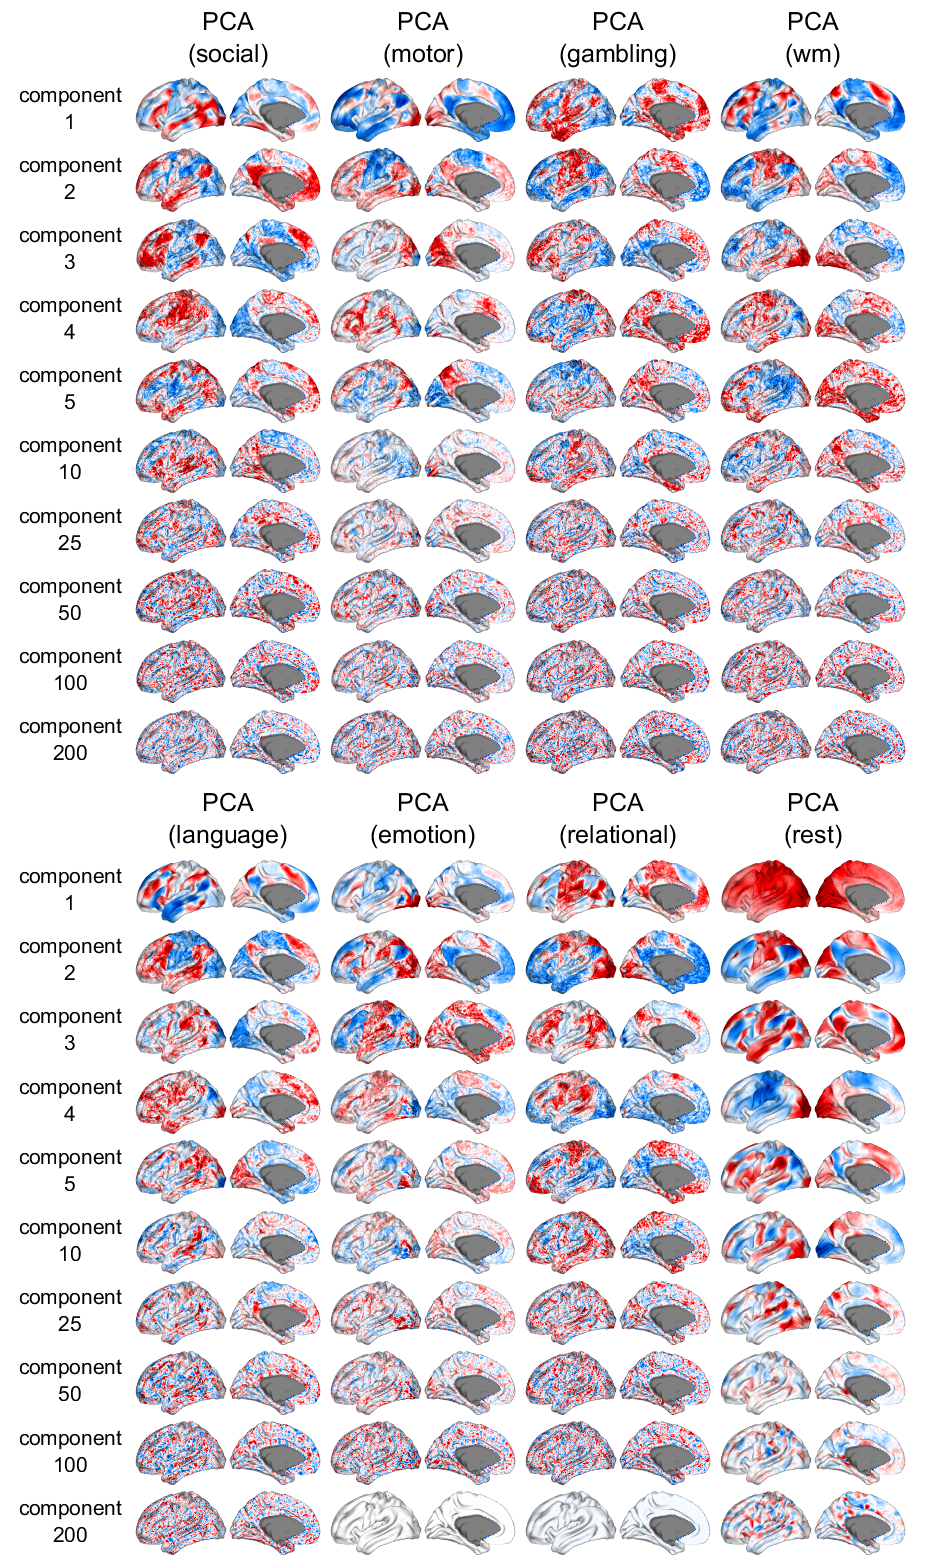
\includegraphics[width=0.85\textwidth]{fig/supp_9.pdf}
	\caption{
	} \label{fig:supp_9}
\end{figure}



\begin{figure}[!htb] 
	\centering
	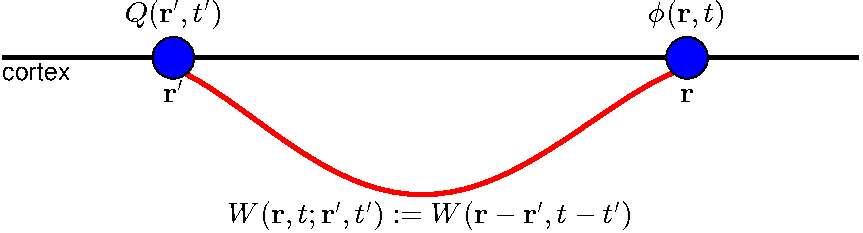
\includegraphics[width=0.85\textwidth]{fig/supp_10.pdf}
	\caption{
	} \label{fig:supp_10}
\end{figure}


\begin{figure}[!htb] 
	\centering
	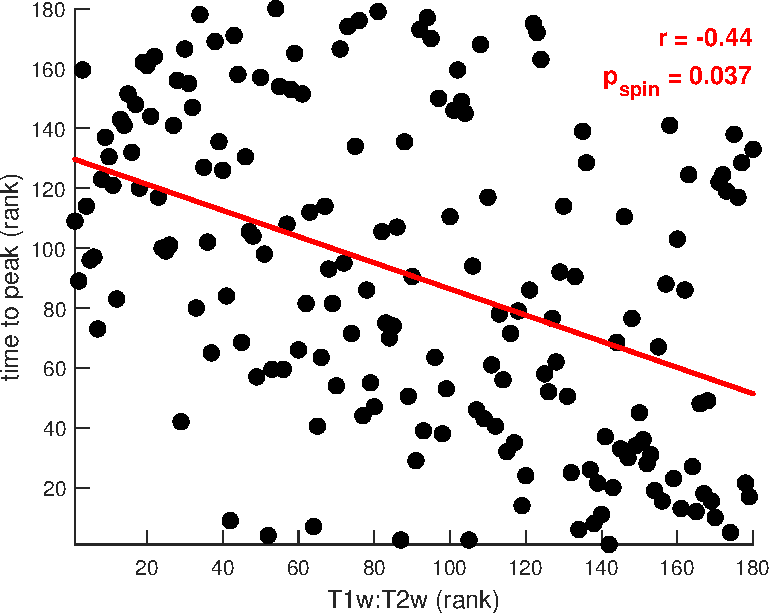
\includegraphics[width=0.85\textwidth]{fig/supp_11.pdf}
	\caption{
	} \label{fig:supp_11}
\end{figure}



%%=============================================%%
%% For submissions to Nature Portfolio Journals %%
%% please use the heading ``Extended Data''.   %%
%%=============================================%%

%%=============================================================%%
%% Sample for another appendix section			       %%
%%=============================================================%%

%% \section{Example of another appendix section}\label{secA2}%
%% Appendices may be used for helpful, supporting or essential material that would otherwise 
%% clutter, break up or be distracting to the text. Appendices can consist of sections, figures, 
%% tables and equations etc.

\end{appendices}

%%===========================================================================================%%
%% If you are submitting to one of the Nature Portfolio journals, using the eJP submission   %%
%% system, please include the references within the manuscript file itself. You may do this  %%
%% by copying the reference list from your .bbl file, paste it into the main manuscript .tex %%
%% file, and delete the associated \verb+\bibliography+ commands.                            %%
%%===========================================================================================%%

\bibliography{sn-bibliography}% common bib file
%% if required, the content of .bbl file can be included here once bbl is generated
%%\input sn-article.bbl

%\bibliography{reference}


\end{document}
